\documentclass[11pt]{book}

%%%% Fill out all these macros
\newcommand{\thesisTitle}{Data analysis tools for statistical non-experts}
\newcommand{\authorName}{Eunice Jun}
\newcommand{\advisor}{Jeffrey Heer}
\newcommand{\advisorTitle}{Jerre D. Noe Endowed Professor} % assistant, associate prof?
\newcommand{\advisorDepartment}{Paul G. Allen School of Computer Science \& Engineering}
% if you have two advisors, uncomment these two
\def\rene{Ren\'{e}\xspace}
\def\reneJust{Ren\'{e} Just\xspace}
\newcommand{\secondAdvisor}{\reneJust}
\newcommand{\secondAdvisorTitle}{Associate Professor}
\newcommand{\secondAdvisorDepartment}{Paul G. Allen School of Computer Science \& Engineering}

\newcommand{\readingCommitteeOne}{Tyler H. McCormick}
\newcommand{\graduationYear}{2023}

%\usepackage{} -- add any other packages you want
%\usepackage{proceed2e}
\usepackage[hyphens]{url}
\usepackage{amsfonts}
\usepackage{multirow,tabularx}
\usepackage{listings}
\usepackage{makecell}
\usepackage[linesnumbered]{algorithm2e}
\usepackage{amssymb}
\usepackage{graphicx}
\usepackage{amsmath}
\usepackage{float}
\usepackage{fullpage}
\usepackage{mathrsfs}
\usepackage{subcaption}
\usepackage{hyperref}% http://ctan.org/pkg/hyperref
\hypersetup{%
  %colorlinks = true,
  linkcolor  = black
}
\usepackage{mdwlist}
\usepackage{xspace}
\usepackage{setspace}
% \usepackage{times} % Set the typeface to Times Roman
\usepackage[scaled]{helvet} % ss
\usepackage{courier} % tt
\normalfont
\usepackage[T1]{fontenc}
\usepackage[utf8]{inputenc}
% \usepackage[cp1251]{inputenc}


%\usepackage[showframe=true]{geometry}
\usepackage{changepage}
\usepackage[labelfont=bf]{caption} % boldface caption title for floats
\usepackage[square]{natbib}
\usepackage{enumitem}
\usepackage{natbib}
\setcitestyle{numbers}
\usepackage{array,multirow}
\usepackage{fixltx2e}
\usepackage{booktabs}
\usepackage{bbm}
\usepackage{soul}
\usepackage{relsize}
\usepackage{eso-pic}
\usepackage{xspace}
\usepackage{epsfig}
\usepackage{graphicx}
\usepackage{amsmath}
\usepackage{amssymb}
\usepackage{float}
\usepackage{multirow}
\usepackage{rotating}
\usepackage{balance}
\usepackage{wrapfig}
% \usepackage{enumerate}
\usepackage{caption}
\usepackage{framed}
\usepackage{enumitem}
\usepackage{multirow}
\usepackage{graphicx}
\usepackage{color}
\usepackage{fixltx2e}
% \usepackage{tkz-graph}
\usepackage{caption}
\usepackage{subcaption}
\usepackage{tikz}
\usepackage{mathtools}
\usepackage{pifont}
\usepackage{scrextend}
\usepackage{sidecap}
\usepackage{graphicx}
\usepackage{comment}
\usepackage{longtable} % for long tables
% For uniform capitalization of section titles
% \usepackage{sectsty}
\usepackage{titlecaps}
% \sectionfont{\titlecap}
\let\oldsection\section
\renewcommand{\section}[1]{\oldsection{\titlecap{#1}}}
\Addlcwords{and or of as on in with rTisane for} % Keep these words lowercase
% \let\oldsubsection\subsection
% \renewcommand{\subsection}[1]{\oldsubsection{\titlecap{#1}}}


% For Tikz graphics
\usepackage{tikz}
\usetikzlibrary{positioning,arrows.meta,graphs,backgrounds,fit,calc,quotes,shapes.multipart}
\usepackage{pgfplots}
\usepackage{pgfplotstable}

\usepackage{todo} % for todo list
\newcommand{\ej}[1]{\colorbox{blue!30}{#1}}
\newcommand{\highlight}[1]{\colorbox{yellow!30}{\textit{#1}}}
\newcommand{\polish}[1]{\colorbox{yellow!30}{#1}}
\newcommand{\revisit}[1]{\textcolor{orange}{Revisit: #1}}

% For changing size of text in Acknowledgements
% \newenvironment{localsize}[1]
% {%
%   \clearpage
%   \let\orignewcommand\newcommand
%   \let\newcommand\renewcommand
%   \makeatletter
%   \input{bk#1.clo}%
%   \makeatother
%   \let\newcommand\orignewcommand
% }
% {%
%   \clearpage
% }

%%%%%% For consistent terminology 
% Tea 
\def\tea{Tea\xspace}
\def\TeaPL{Tea's programming language\xspace}
\def\TeaRS{Tea's runtime system\xspace}

\def\dataSet{dataset\xspace}
\def\dataSets{datasets\xspace}

% Hypothesis formalization 
%% Quotes
\newcommand{\shortquote}[1]{``\emph{#1}''}
\newcommand{\longquote}[1]{\vspace{-1pt}\begin{quote}``\emph{#1}''\end{quote}}
\newcommand{\theme}[1]{\vspace{-1pt}\subsubsection{Theme: #1} }
\newcommand{\groupingtheme}[1]{\subsubsection{\textbf{#1}} }
%% Research Questions
\def\rqSteps{\textbf{RQ1 - Steps}\xspace}
\def\rqProcess{\textbf{RQ2 - Process}\xspace}
\def\rqTools{\textbf{RQ3 - Tools}\xspace}

% Tool Implications
\def\higherLevel{\textit{DI1 - Raise level of abstracion}\xspace}
\def\connectConceptualStats{\textit{DI2 - Connect conceptual and statistical models}\xspace}
\def\relateStats{\textit{DI3 - Relate statistical methods}\xspace}

% Tisane terminology
\def\tisane{Tisane\xspace}
\def\rTisane{rTisane\xspace}
\def\rTisanes{rTisane's\xspace}
\def\Disambiguation{Disambiguation\xspace}
\def\disambiguation{disambiguation\xspace}
\def\SDSLlong{study design specification language\xspace}
\def\SDSL{SDSL\xspace}

% rTisane summative eval 
%% Evaluation Research Questions
\def\evalConceptualModels{\textbf{RQ1 - Conceptual models}\xspace}
\def\evalStatisticalModels{\textbf{RQ2 - Statistical models}\xspace}
\def\evalLearning{\textbf{RQ3 - Learning}\xspace}

% Hypothesis formalization 
\def\hypoForm{\textit{hypothesis formalization}\xspace}
\def\HypoForm{\textit{Hypothesis formalization}\xspace}

%% Evaluation Research Questions
\def\rqWorkflow{\textbf{RQ1 - Workflow}\xspace}
\def\rqCognitive{\textbf{RQ2 - Cognitive fixation}\xspace}
\def\rqFuture{\textbf{RQ3 - Future possibilities}\xspace}

%% Design considerations
\def\dcConceptualKnowledge{\textit{DG1 - Conceptual knowledge}\xspace}
\def\dcConceptualKnowledgeLong{\textit{DG1 - Prioritize conceptual knowledge.}\xspace}
\def\dcValidity{\textit{DG2 - Validity}\xspace}
\def\dcValidityLong{\textit{DG2 - Prioritize the validity of models.}\xspace}
\def\dcGuidance{\textit{DG3 - Guidance and control}\xspace}
\def\dcGuidanceLong{\textit{DG3 - Give analysts guidance and control.}\xspace}
\def\dcStatisticalPlanning{\textit{DG4 - Statistical planning}\xspace}
\def\dcStatisticalPlanningLong{\textit{DG4 - Facilitate statistical planning without data.}\xspace}

% Tool Implications
\def\higherLevel{\textit{DI1 - Raise level of abstracion}\xspace}
\def\connectConceptualStats{\textit{DI2 - Connect conceptual and statistical models}\xspace}
\def\relateStats{\textit{DI3 - Relate statistical methods}\xspace}

%% Other
\def\lme{\texttt{lme4}\xspace}
\def\statsmodels{\texttt{statsmodels}\xspace}
\def\pymer{\texttt{pymer4}\xspace}
\newcommand\upquote[1]{\textquotesingle#1\textquotesingle}
%% Referencing sections
\def\sectionautorefname{Section}
%% Referencing subsections
\def\subsectionautorefname{Subsection}
%% Referencing chapters 
\renewcommand{\chapterautorefname}{Chapter}
%% Other useful macros and abbreviations
\def\etal{et al.\xspace}
%% Qualitative analysis
\def\codebook{codebook\xspace}


%%%%%% For publications
\newcommand{\uistConf}[1]{\textit{ACM UIST #1}}
\newcommand{\chiConf}[1]{\textit{ACM CHI #1}}
\newcommand{\tochi}[1]{\textit{ACM Transactions of Computer-Human Interaction (TOCHI) #1}}


%$%%%% Macros for consistent typesetting of tables.

% Minimizing spacing for tables
\usepackage{setspace}


%% Fix spacing in non-right-aligned columns
\newcommand{\z}{\phantom{0}}

%% Shortcut for plus/minus sign
\newcommand{\p}{$\scriptsize{\pm}$}

%% Always center and bold face column headers
\newcommand\colH[1]{\multicolumn{1}{l}{\textbf{#1}}}
\newcommand\colHR[1]{\multicolumn{1}{r}{\textbf{#1}}}
\newcommand\colsH[2]{\multicolumn{#1}{c}{\textbf{#2}}}

%% New column type to "hide" a column
%\newcolumntype{H}{>{\setbox0=\hbox\bgroup}c<{\egroup}@{}}

%% Typeset an assumption
\newcommand{\assume}[1]{\tikz[baseline]\node[circle,inner xsep=2pt,inner ysep=0pt,
        draw=black,fill=white,scale=0.8,anchor=base] {#1};}
%% Typeset a valid assumption
\newcommand{\valid}[1]{\tikz[baseline]\node[circle,inner xsep=2pt,inner ysep=0pt,
        draw=black,fill=gray!50!white,scale=0.8,anchor=base] {#1};}
%% Typeset an invalid assumption
\newcommand{\invalid}[1]{\tikz[baseline]\node[circle,inner xsep=2pt,inner ysep=0pt,
        draw=black,fill=white!30!white,scale=0.8,anchor=base] {#1};}
\def\yes{$\checkmark$}
\def\no{---}

%%%%%%%%%%%%%%%%%%%%%%%%%%%%%%%%%%%%%%%%%%%%%%%%%%%%%%%%%%%%%%%%%%%%%%%%%%%%%%%%
%% Use \<name> or \codeid{name} for source-code related identifiers
\def\<#1>{\codeid{#1}}
\newcommand{\codeid}[1]{\ifmmode{\mbox{\small\ttfamily{#1}}}\else{\small\ttfamily #1}\fi}
\newcommand{\codeidsmall}[1]{\ifmmode{\mbox{\smaller\ttfamily{#1}}}\else{\smaller\ttfamily #1}\fi}


\makeatother


\begin{document}

%% Replace all of the orange portions with your personal info

\begin{titlepage}
\begin{center}
\vspace*{\fill}
\singlespace
\thispagestyle{empty}
{\LARGE { \thesisTitle \\} %self-explanatory
\doublespacing
\vspace*{\baselineskip}
{\large \authorName }\\ %self-explanatory
\vspace*{1.5\baselineskip}
\large A dissertation
\\ submitted in partial fulfillment of the\\
requirements for the degree of\\
\vspace*{\baselineskip}
Doctor of Philosophy\\
\vspace{1.5\baselineskip}
University of Washington
\\ \graduationYear}\\ % add year in YYYY format (e.g. 2020)
\vspace{1.5\baselineskip}

%add reading committee (just the reading committee, not the supervisory committee):
\large \textit{Reading Committee:} \\

\ifdefined\secondAdvisor 
    \advisor, Co-Chair \\
    \secondAdvisor, Co-Chair \\
\else
    \advisor, Chair
\fi

\readingCommitteeOne \\

\ifdefined\readingCommitteeTwo
    \readingCommitteeTwo \\
\fi

\ifdefined\readingCommitteeThree
    \readingCommitteeThree \\
\fi
    

\vspace{2\baselineskip}
  Program Authorized to Offer Degree: \\
Paul G. Allen School of Computer Science \& Engineering
  
% \newcommand{\advisor}{Main Guardian}
% % if you have two advisors, uncomment these two
% \newcommand{\firstAdvisor}{Parent One}
% \newcommand{\secondAdvisor}{Parent Two}
% \newcommand{\readingCommitteeOne}{First Reader}
% \newcommand{\readingCommitteeTwo}{Second Reader}

  
  
%%% Insert year and name:
  \vspace*{\fill}
  \clearpage
  \thispagestyle{empty}
  \singlespace{
  \copyright~Copyright \graduationYear \\ %add year in YYYY format (e.g. 2020)
  \vspace*{\baselineskip}
  \authorName} %self-explanatory
\end{center}
\end{titlepage}


\doublespacing

%% Replace all of the orange portions with your personal info

\thispagestyle{empty}
\begin{centering}
\vspace{1in}
University of Washington \\
\vspace*{1.\baselineskip}
{\bf Abstract}\\
\vspace*{1\baselineskip}

{\thesisTitle}\\ %self-explanatory
\vspace*{1.\baselineskip}
{\authorName} \\ %self-explanatory
\vspace*{1.\baselineskip}


\ifdefined\secondAdvisor
    Co-chairs
    \else
    Chair
\fi
of the Supervisory Committee:\\ %change to co-chair if co-advised 
\advisorTitle~\advisor\\ \vspace{-.5em} \advisorDepartment \\
\ifdefined\secondAdvisor
    \secondAdvisorTitle~\secondAdvisor\\\vspace{-.5em}\secondAdvisorDepartment \\
\fi
\end{centering}
\vspace*{\baselineskip}

\polish{Easy: Make sure all participant references in square brackets} \\
\polish{Easy/Medium: Check refs that should be autorefs!! by searching and replacing} \\
\polish{Easy: Make sure no space after rTisane or Tisane before ', search in PDF} \\
\polish{Easy: Make sure that the appropriate sections show up in TOC + add section/section*} \\
\polish{Easy/Medium: Pass through to make sure that all figures/tables are consistent} \\
\polish{Medium/Hard: Check that all figures/tables have caption + formatted consistently} \\
\polish{Medium: Call out specific challenges in Summary of Contributions at the end of each chapter} \\
\polish{Medium/Hard: Decide if going to split Tisane/rTisane up ==> Change} \\
\polish{Final pass: Read over acknowledgements} \\
\polish{Final pass: Page formatting: > Page 26 of the PDF is blank and could be removed. This recurs elsewhere in the document (for example on page 50 and page 84). It's not clear to me if this is intentional.} \\
\polish{Final pass: Formatting: Margins all ok} \\

Data analysis is critical to science, public policy, and business. Despite their
importance, statistical analyses are difficult to author, especially for
researchers with expertise outside of statistics. Existing statistical tools,
prioritizing mathematical expressivity and computational control, are low-level
while researchers' motivating questions and hypotheses are high-level.
Researchers need to translate their questions and hypotheses into low-level
statistical code in an error-prone process. 
% This thesis views statistical analysis authoring as an end-user software
% engineering problem.
This thesis views statistical analysis authoring as a sensemaking process that
involves grappling with domain knowledge, statistics, and programming concerns.
To this end, I develop a framework characterizing the cognitive and operational
steps involved in translating research questions into statistical analysis code,
which I call \hypoForm. I also design, implement, and evaluate two new DSLs and
runtimes that embody \hypoForm. The DSLs leverage automated reasoning to compile
high-level specifications of analysis intent into analysis code.

The first of these is \tea for authoring Null Hypothesis Significance
Tests. Analysts specify their study design, assumptions about data, and
hypotheses in \tea's DSL. \tea represents statistical test selection as
constraint satisfaction, so it compiles an analyst's specification into a system
of constraints to identify a set of valid statistical tests. A benchmark
comparison found that \tea's test selection is comparable to that of experts and
better than a naive test selection approach. 

This dissertation also introduces \tisane for authoring generalized linear
models with or without mixed effects. Analysts specify their domain knowledge in
the form of a conceptual model, data collection details, and focus of analysis
in \tisane's DSL. Internally, \tisane represents this conceptual model as a
graph, which it traverses to derive a space of statistical models based on
causal reasoning recommendations. Then, in an interactive disambiguation
process, \tisane involves analysts in narrowing the space of possible
statistical models to one final output statistical modeling script. In case
studies, we found that \tisane shifted researchers' focus from analysis details
to their research questions and streamlined the analysis authoring process. To
further improve the usability of the \tisane DSL, I conducted an exploratory
elicitation study using \tisane as a probe, re-designed and re-implemented
\tisane in R as \rTisane, and then evaluated \rTisane in a controlled lab study.
The summative evaluation demonstrated that \rTisanes DSL helped analysts
introspect on their implicit domain assumptions more deeply, stay true to their
analysis intent, and produce statistical models that better fit the data. In
all, these systems and evaluations provide evidence that conceptually focused
DSLs coupled with automated reasoning can lower the barriers to valid analyses.


% This dissertation introduces a new way of authoring analyses two tools that embody a new way of authoring
% analyses: Tea and Tisane. Researchers directly express their domain knowledge
% through higher level abstractions, and the tools will validate the data, select
% a statistical analysis, and implement it, all while educating analysts about why
% a statistical approach is valid. Tea helps analysts author statistical tests.
% Tea's key insight is that  Tisane enables analysts to author generalized linear
% models with or without mixed effects, which are difficult for even statistical
% experts to author. Using Tisane, analysts can express their conceptual models
% using a high-level domain specific language. Tisane translates these conceptual
% models into causal DAGs and engages analysts in a disambiguation process to
% arrive at an output statistical model. Real-world researchers have already used
% these tools to conduct analyses in published research that push their own
% disciplines forward. I will also introduce ``hypothesis formalization,'' a series
% of cognitive and operational steps analysts take to translate their research
% questions into statistical implementations. Hypothesis formalization
% retrospectively explains why Tea improves statistical testing and directly
% inspired the design of Tisane. 

% Tea and Tisane serve as platforms for further research into computational
% support for statistical analysis. This work also exemplifies how combining
% human-computer interaction with other areas in and outside of computer science
% leads to software tools that impact real-world users.


\chapter*{Acknowledgements}
% \begin{localsize}{10}
% \small
I am lucky to have many, many people to thank. 

\textit{I thank my advisors Jeffrey Heer and \reneJust.} Jeff, thank you for
your endless creativity, sense of humor, and focused attention in all our
conversations. Thanks also for helping me navigate personal and professional
challenges with integrity. I had a lot of fun and freedom during the second half of my PhD
thanks to you. \rene, thank you for your consistent insistence on
the details.

% \item Committee 
\textit{I have the best committee, hands down.} Emery Berger, I am deeply grateful
that you agreed to meet with me, then a total stranger, at the start of your
sabbatical at MSR in 2018. Who knew that coffee would lead to many, many
more espressos while we worked on Tea, Scone, and a number of other projects. You have been my most ardent
champion and creative conversational partner. Thank you for including me in on your latest crazy idea and laughing with me
through the highs and lows of graduate school. 
% Thank you for always keeping
% me updated on your latest crazy idea and bringing me into projects. Your
% support through the highs and lows of graduate school, always with a heavy
% bout of laughter, kept me going. 
% Emery, you may be the best mad scientist I know, but above all,
% you are the strongest advocate I could have asked for. 
Leilani Battle, thank you for your enthusiasm and support since you were a
postdoc at UW! It's great to have you back.    
Tyler McCormick, thank you for welcoming me into your research group and the
Center for Statistics and the Social Sciences (CSSS). Our conversations and
collaboration have expanded my thinking and scholarship. 
% \item IDL, PLSE, Zach 

\textit{I am grateful to have been part of the warm UW CSE community throughout
my PhD.} In particular, I am indebted to the members of the Interactive Data Lab
(IDL) with whom I overlapped during my PhD for their camaraderie: Arvind
Satyanarayan, Ham Wongsuphasawat, Dominik Moritz, Yeaseul Kim, Younghoon Kim,
Jane Hoffswell, Sherry Wu, Alex Kale, Yang Liu, Matt Conlen, Zening Qu, Mick
Kittivorawong, Ameya Patil, Junran Yang, Madeleine Grunde-McLaughlin, Josh
Horowitz, and Luke Snyder. Michael Correll and Maureen Stone, while not students
in IDL, were consistent members of the lab. Thank you, all, for keeping me
humble, honest, and hopeful about the positive social impact of great research
and open-source software.

% In addition to IDL, 
I have also been fortunate to be part of the idiosyncratic PLSE
lab. 
% To my friends in PLSE over the years, of which there are too many to name
% individually, 
% Thank you for all the snacks, heated
% conversations, and tea. 
To my PLSE labmates over the years, of which there are too many to name
individually, I love how ferociously curious and whimsical you are about
everything in research and life. I would not have pursued this
research without PLSE welcoming me early on. In this regard, I want to give
special thanks to my friends Sarah Chasins, James Bornholt, Mangpo Phothilimthana, Sami Davies, Chandra
Nandi, Amanda Swearngin, Chenglong Wang, Jasper Tran O'Leary, Gus Smith, Pavel Panchekha,
and Max Willsey. Zachary Tatlock, thank you for investing so much of yourself
into making PLSE the best place to pursue daring research, have fun, and make
friends. 

To Elise Dorough, thank you for everything you do to keep CSE running while
still making time to help my peers and me through any situation (and many
emotions). To Joe Eckert, thank you for answering my numerous Slack messages
and cries for help even when I caused my own logistical problems. To
Elle Brown, thank you for your kindness. To Lisa Merlin, thank you for
helping me with countless reimbursements and doing everything in your power
to protect me from bureaucratic processes.

% To my CSE 492 (?) officemates, especially James Bornholt and Callie Bee, thank
% you for sharing in many humorous memories. 
\textit{The larger UW ecosystem has also shaped my scholarship.} To the members
of CSSS, thank you for welcoming me and giving me many opportunities to learn
from and ask questions of scholars across the social and statistical sciences.
The interdisciplinary seminars and courses, such a Thomas Richardson's offering
of CSSS/STAT 566 on causal reasoning, were instrumental in my graduate
education. Thanks also to the larger HCI community in DUB. There are a few
individual mentors to whom my gratitude is overdue: Daniela Rosner (HCDE), Tim
Althoff (CSE), and Amy Ko (iSchool). To Daniela, especially, thank you for
sharing your brilliance, wisdom, and curiosity about ``design'' and life over
memorable chats in your office and on walks throughout the city. 
% I have been incredibly lucky to have mentors across
% campus. To Daniela Rosner, whose encouragement and mentorship during my PhD
% is long overdue, thank you for sharing your curiosity, creativity, and
% humor. To Tim Althoff, thank you for our brainstorming sessions to explore
% research ideas. 

% \item MSR internship mentors: Mary, Daniel, Ben 
\textit{During my PhD, I had so much fun and expanded my research horizons
through two summer internships at Microsoft Research.} Mary Czerwinski, Daniel
McDuff, and Ben Zorn, thank you for entrusting me to run with new ideas,
modeling constructive mentorship (which I strive to emulate), and becoming
friends over the years. 

% \item Mentees 
% \item IHME collaborators, CSSS 
\textit{To my collaborators, thank you, for your inspiration, energy, and support.}
Specifically, I thank Joseph Dieleman and Goli Tsakalos, for inviting me as
a volunteer with the Institute for Health Metrics and Evaluation (IHME) the
last two years of my PhD. To Sawyer Crosby and Emily Johnson, thank you for
your time and energy in showing me the ropes at IHME, sharing your analysis
experiences, and trying out and giving helpful feedback on early prototypes
of my systems. To Maureen Daum, thank you for your candor, reliability, and
sense of humor as a collaborator and friend. To Nicole de Moura, Grace Oh,
Melissa Birchfield, Pranav Rajan, Shreyash Nigam, Josh Pollock, Annie
Denton, Blue A. Jo, Reiden Chea, Corinne Herzog, Vincent Pun, Irene Luo, Ken
Gu, Audrey Seo, and Edward Misback, thanks for entrusting me to mentor you during your
explorations of research and computer science. I am so immensely proud of
how you have pursued your interests, and I look forward to seeing
you continue to grow!

\textit{I would not have pursued a PhD without formative mentorship and research
experiences as an undergraduate}. I thank my undergraduate advisors Bobby
Bodenheimer and John Rieser for encouraging me to embody and live out my
curiosities. To Richard Paris and Lauren Buck, my cool graduate student
labmates, thank you for your friendship and memorable dinner parties. To my REU
mentors at the University of Utah, Bill Thompson, Sarah Creem-Regehr, and
Jeanine Stefanucci, thank you for inviting me into your lab, sharing about life
and research with candor, and modeling collaboration and leadership. To Shashank
Pandey and Jubi Taneja, thank you for sharing poetry, meals, and laughter as we
became friends that formative summer at Utah.

% \item UW CSE + DUB, Daniela, Tim; officemates + batchmates; Elise, Joe, Elle, Lisa; Maureen (co-author)
% \item Council of Wise Women: Advent Anglican, St. Mark's gardening club, Seattle Mosaic Arts
\textit{I am immensely grateful to my community in and around Seattle.} To my
Council of Wise Women from Advent Anglican (especially Kristina Bresnen),
Seattle Mosaic Arts (I hear you laughing, June Chang and Claire Barnett!), and
St. Mark's Gardening Ministry (especially Kathy Sodergren, Kelly Lundquist,
and Kathy Thomason), thank you for enriching my soul. You have shared so much wisdom
in the countless hours I have sat in your presence, often in silence.
% even if there were no words exchanged. 
% , sometimes
% praying, piecing together mosaics, or pulling weeds (what is the
% difference?)

% \item The Emily Program; Patrice; Carrie and Traig and DBT group at Hall Health 
% I give my heartiest, warmest thank you to ``The Emotional B*tches
My heart is beyond a five on the fullness scale, overflowing with marbles for the
``The Emotional B*tches (Thoughts-Emotions-Behaviors)'' and the healthcare
professionals at The Emily Program. 
% You know who you are. 
% who made me laugh, rode
% the elevators up and down one floor with me, and created a true fellowship.
% Our fervor for life (and death) was palpable in everything. 
% beyond full full, overflowing with marbles. 
% My heart is beyond a 5 on the fullness scale. It's overflowing with marbles.
% I can still picture the group room on the eighth floor and incredible view
% of the duck dash on Lake Union every Tuesday night. 
Thank you for creating a true fellowship and, quite literally, keeping me alive.
Patrice Staiger, Carrie DeMartini, and Bethany Bylsma, thank you for guiding me
to, through, and from The Emily Program. Treg Isaacson, Hui Sun, and the others 
% I encountered 
at Hall Health, thank you for lighting the way.
% thank you for being points of light guiding my
% path.
% brightening my path
% always. 

% \item Friends, Besties 
\textit{I thank my friends and family.} To Bridget Claborn, thank you for your
incisive questions, belief in the poetry within and all around us (i.e.,
post-post-modernism, dahlias, anemones, Mary Oliver), and commitment to weave
together research and practice for social change, for life.
%to feel and live in the poetry of the universe. 
To Aoife Blacklaws, thank you for encouraging me in all my endeavors and sharing
your awe of every little creature. To Michael Zuch, thank you for sharing in the
tender, unanswerable questions of faith, theology, and the meaning of life. To Rachael
Grenfell-Dexter, thank you for sharing many adventures around the world and giving me permission to have fun, grow, and evolve. 
To Lucy Rahner, thank you for sharing your artistry and earnest search for the truth and
goodness in everything. To Catherine Chung, thank you for keeping it real,
talking with me endlessly for days, and listening so whole-heartedly. 
To Maria Ventura, thank you for being quick to laugh, judging a person's character based on their pasta, and inspiring me in research.
To Morelle Arian, thank you for welcoming me into your family and sharing your delight in wherever life takes us. 
To Olivia Bradley-Skill, thank you for encouraging me to lean into my creativity and explore ways of combining my interests ever since we were kids.
To the friends named and unnamed, I am honored to share this life with you. 
%incredible earth, even for a brief moment in time. %--how impeccable. 

% \item Partner, Family 
% and fight for
Finally, to Jared Roesch, thank you for your love, commitment to community,
and ambition to focus on what truly matters. To my parents Ok Za Julie and Stephen Jun,
thank you for your sacrifices and support. I love that you
encourage me to write better, more papers even when, by your estimation,
no one reads them.
% \end{itemize}
% \end{localsize}

% Advisors
% Emery

% CSSS, Tyler

% Committee

% I've been lucky to have the counsel of wise women in Seattle. 
% Kristina, Alison, Deborah
% St Mark's - gardening group
% Seattle Mosaic Arts

% The Emily Program - thank you for keeping me alive. 
% Use initials to refer to specific people
% I swear, our daily meals are amazing sources of inspiration for comedy.
% Cursing in my internal monologue

% IDL 

% PLSE

% Mentors - Zach, Daniela Rosner

% MSR - Mary, Daniel, Ben

% IHME 

% Mentees
% ....

% Larger research community
% CSE community - Elise, Joe, Lisa Merlin

% Friends: Irene, Sharon, Elayne B
% Sarah Chasins, James Bornholt, Max Willsey, Sami Davies, Daniel Epstein, Elena Agapie, Ravi Karkar, Jessie Schroeder
% Jina 

% Co-authors of this work - Maureen Daum; Nicole, Melissa

% Besties
% Bridget, Aoife, Rachael, Michael

% Partner, Family
% Write Korean - what Mr. Pama said about baksa in our family
%% Replace all of the orange portions with your personal info

\clearpage

% if you need an extra blank page to make the dedications start on an odd number, then un-comment the following:
\clearpage\thispagestyle{empty}\mbox{}\clearpage 

\begin{center}
% {\LARGE \textbf{DEDICATION}}
{\textbf{DEDICATION}}
\hspace{0pt}
\vfill
%add whomever you want here
% To all the wild women who have danced with me. I promise to never stop. 
To the wild women in my life \\
who got off the speeding train \\ 
to nowhere \\
and are dancing on the platform and \\
throughout the grove -- \\
you know who you are. 
\vfill

% Add or replace with something from Toni or Mary?

\raggedright{i stand} \\
\raggedright{on the sacrifices} \\
\raggedright{of a million women before me} \\
\raggedright{thinking} \\
\raggedright{\textit{what can i do}} \\
\raggedright{\textit{to make this mountain taller}} \\
\raggedright{\textit{so the women after me}} \\
\raggedright{\textit{can see farther}} \\
\raggedright{\textit{- legacy}} \\
\raggedright{Rupi Kaur}

\vfill
\raggedright{There is a special place in hell for women who don't help other women.} \\
\raggedright{Madeleine Albright}
\vfill
\hspace{0pt}
\end{center}



\tableofcontents{}
\listoffigures
\listoftables
\clearpage

\chapter {Introduction}
This chapter typically includes: 
\begin{itemize}
    \item a brief overview
    \item a challenges section
    \item a section about your approach
    \item a section (or subsection in the approach section) giving a dissertation outline (a roadmap of the rest of the thesis)
\end{itemize}

% Data analysis is ipmortant for a number of domains. <Examples> 
Statistical analysis plays a critical role in how people evaluate data and make
decisions. Policy makers rely on models to track disease, inform health
recommendations, and allocate resources. Scientists develop, evaluate, and
compare theories based on statistical results. Journalists report on new
findings in science, which individuals use to make decisions that impact their
nutrition, finances, and other aspects of their lives. Faulty statistical models can lead to spurious estimations of disease spread,
findings that do not generalize or reproduce, and a misinformed public. 
% As data science and statistical analysis has and continues to become more
% prevalent, the number of analysis authors who are not statistical experts will
% increase. 

Despite the prevalence of statistical analyses and their central importance to a
number of disciplines, they remain challenging to author accurately. The key
challenge in developing accurate statistical models lies not in a lack of access
to mathematical tools, of which there are many (e.g., R~\cite{team2013r},
Python~\cite{sanner1999python}, SPSS~\cite{spss}, and SAS~\cite{sas}), but in
accurately applying them in conjunction with domain theory, data collection,
statistical knowledge, and programming ability~\cite{mcelreath2020statistical}.
Analysts must translate their implicit domain knowledge into statistical models
that they can then implement and execute in code. However, this process---which
requires disciplinary, statistical, and programming expertise---is out of reach
for statistical non-experts who depend on accurate analyses, including many
researchers. 
% This process requires
% expertise in a discipline, statistics, and programming.
% Analysts must integrate multiple knowledge sources to specify statistical
% analyses. Yet, this integrative process is out of reach for statistical
% non-experts who depend on accurate analyses, including many researchers. 


\addcontentsline{toc}{section}{Approach}
\section*{Approach}
This dissertation asks if separating the above concerns and incorporating
automated reasoning in statistical software could benefit statistical
non-experts. Towards this goal, I combine techniques from human-computer
interaction, programming languages/software engineering, and statistics to (i)
characterize the cognitive and operational steps to author statistical analyses
and (ii) develop novel interactive systems that enable statistical non-experts
to author valid analyses. As detailed below, I not only move between systems
building and empirical studies but use each to deepen and enhance the other.

The work described in the dissertation demonstrates the following:% thesis statement: 
\addcontentsline{toc}{section}{Thesis statement}
\paragraph{Thesis statement}
% Centered on the insight that domain experts using statistical methods are
% focused on their domain 

%%% COULD MAKE THIS STRONGER?
Domain-specific languages that provide abstractions for expressing conceptual
knowledge, data collection procedures, and analysis intents instead of specific
statistical modeling decisions coupled with automated reasoning to compile
conceptual specifications into statistical analysis code help statistical
non-experts more readily author valid analyses. 

Three challenges fall out of this thesis statement: 

\addcontentsline{toc}{section}{Challenge 1}
\section*{Challenge 1: How to make implicit domain knowledge explicit.} %- domain knowledge
Designing abstractions focused on conceptual knowledge requires identifying what
domain knowledge analysts want and can express and balancing these constraints
with what automated reasoning approaches may require. What is easy to express
and what is easy to assume for the sake of automation may be at odds, especially
when analysts provide ambiguous specifications that could be compiled into
multiple statistical analyses. The challenge therefore, is to design language
constructs that are usable for analysts and useful for automated reasoning and
support interactive program specification as necessary.

% Finding: interactive disambiguation not just necessary for refinement and automated reasoning but *useful* to analysts for reflection

% Shifting focus onto the goal/motivation of analysis and less on the details that can overwhelm and restrict analysts

% **Not just higher levels of abstraction but appropriate abstractions that allow analysts to dig deeper into the appropriate parts

\addcontentsline{toc}{section}{Challenge 2}
\section*{Challenge 2: Represent and reason about key statistical analysis decisions} %- programming
A central idea in this thesis is that software systems should take on the
responsibility of translating conceptual knowledge into statistical analyses.
This is akin to a compilation process that requires representing the conceptual
knowledge analysts express and reasoning over it to derive statistical
analyses that respect statistical best practices and rules. A
major challenge is in picking representations so that the reasoning is straightforward. 
% not only straightforward but also beneficial in someway (expressivity, extensibility for both Tea and Tisane)

\addcontentsline{toc}{section}{Challenge 3}
\section*{Challenge 3: Increase analysts' statistical knowledge/understanding} %- statistics
% connect to Bellotti on user control?
While automating statistical analysis can be helpful, analysts relying on data
to make high-impact decisions (e.g., policy, scientific discovery) often need to
understand why an analysis approach is appropriate and what the implications of
the results are to their domain. Furthermore, software can inform how users
approach future analyses. Therefore, educating analysts about the applicability
and impact of statistical decisions and guiding their interpretation of results
are important.

\addcontentsline{toc}{section}{Summary of Contributions}
\section*{Summary of Contributions}
\ej{Add overview figure from reserach statement}
% Contributions: systems, empirical, and the beginnings of methodological innovation.
This dissertation makes systems and empirical contributions. Additionally, the
process of designing and developing domain-specific languages for end-users
shows the first steps towards developing methods for user-centric language
design. 
% we also explored new methods for eliciting and integrating user
% feedback throughout programming language design.

Specifically, I designed and implemented two systems, Tea~\cite{jun2019tea} and
Tisane~\cite{jun2022tisane}, that leverage \textbf{domain-specific languages}
(DSLs) to capture analysts' implicit assumptions and conceptual knowledge. Users
\textbf{interactively compile} these high-level specifications into low-level
code. To infer valid statistical analyses, the systems \textbf{programmatically
represent and reason about core statistical authoring challenges} as constraints
and graphs (\autoref{fig:tools}).
% As a result, my systems prevent common analysis
% mistakes~\cite{jun2019tea,jun2022tisane}. 

In summary, this dissertation's key contributions are
% The contributions of this research are as follows: 
\begin{itemize} 
    % Whereas hypothesis formalization has remained implicit in prior
    % descriptions of data analysis, we explicate this specific process. 
    \item a \textbf{formal constraint-based model} to specify and select among
    common Null Hypothesis Statistical Tests in Tea (see~\autoref{chapter:tea}); 
    \item empirical findings of how authoring analyses requires integrating
    conceptual, data, statistical, and programming expertise, which we summarize
    in our \textbf{theory of hypothesis formalization} (see~\autoref{chapter:hypoForm}); 
    \item an analysis of how the current statistical software ecosystem does not
    explicitly support and may even hinder hypothesis formalization, suggesting
    new \textbf{design opportunities and implications} (see~\autoref{chapter:hypoForm});
    \item a \textbf{mixed-initiative approach} for ``interactively compiling''
    linear models from conceptual and data relationships in Tisane; 
    \item empirical \textbf{findings on researchers' implicit semantics of
    conceptual models} (see~\autoref{chapter:tisane});
    \item \textbf{new language constructs and interaction methods} for
    reflecting on and refining conceptual models in a second version of Tisane,
    which we call rTisane (see~\autoref{chapter:tisane}); and
    \item qualitative and quantitative \textbf{results showing the benefit of
    recording conceptual models and compiling them into statistical models} in
    rTisane over a scaffolded workflow (see~\autoref{chapter:tisane}).
\end{itemize}

\begin{comment}
\section{Thesis outline}
% System --> Empirical --> System --> Empirical --> Empirical --> System --> Empirical 
This dissertation contributes new domain-specific languages (DSLs) for authoring
statistical analyses and a new theory describing the cognitive and operational
steps involved in authoring statistical analyses. In the process of designing
the second DSL, we also explored new methods for eliciting and integrating user
feedback throughout programming language design. The content of thesis is as
follows. 

\todo{Fill in this outline}

\section*{How to approach this dissertation} \todo{Decide if want to keep}
\end{comment}

\section{Prior Publication and Authorship} \todo{fill in}

\chapter {Related work}
This dissertation builds on theories of sensemaking, empirical findings on
current analytical praxis, and existing tools throughout the data lifecycle.
Additionally, this dissertation uses Donald Campbell's theory of validity to
motivate system designs and interpret evaluation results. Subsequent sections
provide additional background as applicable.

\section{Statistical data analysis as sensemaking}
Human beings engage in \textit{sensemaking} to acquire new knowledge. Several
theories of
sensemaking~\cite{pirolli2005sensemaking,russell1993cost,klein2007dataFrame}
describe how and when human beings seek and integrate new data (e.g.,
observations, experiences, etc.) to develop their mental models about the world.

Russell et al.~\cite{russell1993cost} define sensemaking as ``the process of
searching for a representation and encoding data in that representation to
answer task-specific questions.'' Russell et al. emphasize the importance of
external representations. Sensemaking is the iterative process of searching for
and refining external representations in a ``learning loop complex'' that
involves transitioning back and forth between (i) searching for and (ii)
instantiating representations. External representations are critical because
they influence the quality of conclusions reached at the end of the sensemaking
process and affect how much time and effort is required in the process. Some
representations may lead to insights more quickly. Indeed, we posit and find
that statistical analysis, specifically hypothesis formalization
(\autoref{chapter:hypoForm}), is a learning loop~\cite{russell1993cost} where
the conceptual research question or hypothesis is an external representation of
a set of assumptions analysts may have about the world (e.g., an implicit causal
model), that ultimately affects which statistical models are implemented and
which results are obtained. We also find that there are smaller learning
loops---for revising explicit causal models, mathematical equations, and
partially specified models---embedded in the larger loop of hypothesis
formalization.

Grolemund and Wickham argued for statistical data analysis as a sensemaking
activity~\cite{grolemund2014cognitive}. They emphasize the (1) bidirectional
nature of updating mental models of the world and hypotheses based on data and
collecting data based on hypotheses and (2) the process of identifying and
reconciling discrepancies between hypotheses and data. Similar to Russell et
al., Grolemund and Wickham's model demonstrates the importance of representing
and re-representing conceptual knowledge. Grolemund and Wickham's theory of data
analysis includes a back and forth between an analyst's ``schema'' of how a
phenomenon occurs in the world, a statistical model, and data. Analysts' domain
expertise influence their schemas, which represent conceptual knowledge about
known and unknown causal mechanisms, for example. Analysts' conceptual schema
directly inform their hypotheses, which are statistical predictions represented
in statistical models. These statistical models are then compared to collected
data, and any discrepancies between the data and hypothesis require analysts to
re-examine and possibly update their statistical model, schema, or both.
Extending Grolemund and Wickham's model, our work on hypothesis formalization
differentiates between conceptual and statistical hypotheses and probes the
phases an analyst must go through to encode a conceptual hypothesis into a
statistical model.

Given the centrality of external representations of implicit conceptual
knowledge to authoring statistical analyses that help analysts make sense of
the world, we argue that our statistical software should focus on helping
analysts to express their conceptual hypotheses and implicit domain knowledge.
Through the development of two software systems, \tea (~\autoref{chapter:tea})
and Tisane(~\autoref{chapter:tisane}), we explore \textit{how} to design
programming abstractions and \textit{what} those abstractions should include in
order for statistical non-experts to externalize their implicit conceptual
knowledge about a domain. 

\section{Empirical accounts of data analysis practice}
% In support of this theoretical view of data analysis as sensemaking, studies
% with analysts have found that data analysis is an iterative process that
% involves data collection; cleaning and wrangling; and statistical testing and
% modeling~\cite{kandel2012enterprise,alspaugh2018futzing,wongsuphasawat2019EDAgoals,grolemund2014cognitive,liu2019paths,liu2019understanding}.
% The importance of exploration and its role in updating analysts' understanding
% of the data and their goals and hypotheses is of note. 

Data analysis involves a number of tasks that involve data discovery, wrangling,
profiling, modeling, and reporting~\cite{kandel2012enterprise}. Extending the
findings of Kandel et al.~\cite{kandel2012enterprise}, both Alspaugh et
al.~\cite{alspaugh2018futzing} and Wongsuphasawat et
al.~\cite{wongsuphasawat2019EDAgoals} propose exploration as a distinct task.
Whereas Wongsuphasawat et al. argue that exploration should subsume discovery
and profiling, Alspaugh et al. describe exploration as an alternative
to modeling. The importance of exploration and its role in updating analysts'
understanding of the data and their goals and hypotheses is of note, regardless
of the precise order or set of tasks. Battle and Heer describe
exploratory visual analysis (EVA), a subset of exploratory data analysis (EDA)
where visualizations are the primary interfaces and outputs for exploring data,
as encompassing both data-focused (bottom-up) and goal- or hypothesis-focused
(top-down) investigations~\cite{battle2019EVA}. In~\autoref{chapter:hypoForm},
we found that (i) analysts explored their data before modeling and (ii)
exploratory observations sometimes prompted conceptual shifts in hypotheses
(bottom-up) but at other times were guided by hypotheses and only impacted
statistical analyses (top-down). In this way, data exploration appears to be an
important intermediate step in hypothesis formalization, blurring the lines
between exploratory and confirmatory data analysis. 

Decisions throughout analysis tasks can give rise to a ``garden of forking
paths''~\cite{gelman2013garden}, which compounds for meta-analyses synthesizing
previous findings~\cite{kale2019decision}. Liu, Boukhelifa, and
Eagan~\cite{liu2019understanding} proposed a broad framework that characterizes
analysis alternatives using three different \textit{levels of abstraction}:
cognitive (e.g., shifts in conceptual hypotheses), artifact (e.g., choice in
statistical tools), and execution (e.g., computational tuning).
\textit{Cognitive} alternatives involve more conceptual shifts and changes
(e.g., mental models, hypotheses). \textit{Artifact} alternatives pertain to
tooling (e.g., which software is used for analysis?), model (e.g., what is the
general mathematical approach?), and data choices (e.g., which dataset is
used?). \textit{Execution} alternatives are closely related to artifact
alternatives but are more fine-grained programmatic decisions (e.g.,
hyperparameter tuning). We find that hypothesis formalization involves all three
levels of abstraction and provide a more granular depiction of how these levels
cooperate with one another (\autoref{chapter:hypoForm}). 

Moreover, Liu, Althoff, and Heer~\cite{liu2019paths} identified numerous
decision points throughout the data lifecycle, which they call
\textit{end-to-end analysis}. They found that analysts often revisit key
decisions during data collection, wrangling, modeling, and evaluation. Liu,
Althoff, and Heer also found that researchers executed and selectively reported
analyses that were already found in prior work and familiar to the research
community. The focus of this thesis is on how any single pass or iteration
occurs. We approach this work from the perspective that by understanding a
single iteration, we may be able to focus analysts on their iterations that are
most substantial and impactful and eliminate a number of unnecessary iterations
that arise due to mistakes in aligning conceptual and statistical concerns,
which we found in our case studies (see ~\autoref{sec:tisane_case_studies}).

% Our depiction of hypothesis formalization aims to account for more
% domain-general steps and artifacts, but we recognize that domain expertise and
% norms may determine which paths and how quickly analysts move through hypothesis
% formalization.

Importantly, our work differs in (i) scope and (ii) method from prior work in
HCI on data analysis practices. Whereas translating a research question or
hypothesis into a statistical analysis has remained implicit in prior
descriptions of data analysis, we explicate this specific process. Additionally,
while previous researchers have relied primarily on post-analysis interviews
with analysts, our lab study (\autoref{sec:inLabStudy}) enables us to observe
decision making during this process in-situ.


% Whereas hypothesis formalization
% has remained implicit in prior descriptions of data analysis, we explicate this
% specific process. Furthermore, our work differs in method. While previous
% researchers have relied primarily on post-analysis interviews with analysts, our
% lab study (\autoref{sec:inLabStudy}) enables us to observe decision making
% during hypothesis formalization in-situ. In summary, our work differs in (i)
% scope and (ii) method from prior work in HCI on data analysis practices. 

\section{Tools for data analysis}
The software ecosystem for data analysis is vibrant, with numerous programming
languages, software packages, and graphical-first tools. A common limitation of
existing software is its siloing of statistical specification from the
conceptual and data collection details that inadvertently influence statistical
analysis. In contrast, the systems in this dissertation explore ways to leverage
implicit conceptual and data collection knowledge to derive statistical
analyses. Below, we compare and contrast this dissertation with existing
software for conceptual modeling, study design, and statistical specification. 

% In this dissertation, we explore the levels of abstraction we can
% provide to meet users where they are comfortable (and their goals) while also
% having sufficient information to reason about statistical methods. We also explore
% two different reasoning methods (constraint-based in \tea and graph-based in
% Tisane) and find that a hybrid approach (\teasane) may be the most promising for realizing
% the vision of supporting hypothesis formalization end-to-end.

\subsection{Tools for conceptual modeling}
For statistical experts, causal diagramming is a common approach to
externalizing implicit concpetual models. For instance,
Daggity~\cite{textor2011dagitty} supports authoring, editing, and formally
analyzing causal graphs through code and a visual editor. The key limitation of
Daggity is that it requires analysts to specify a formal causal graph, which
statistical non-experts, including many domain experts, may not be able to
do~\cite{suzuki2020causal,suzuki2018mechanisms,velentgas2013developing}. In
fact, an open challenge for causal reasoning and discovery is in getting domain
experts to express their implicit knowledge in a way that can be formally
represented and reasoned about. Our work on \tisane directly addresses this
challenge. Moreover, even if analysts are able to express causal diagrams in
Dagitty, Dagitty does not translate queries analysts may have about the causal
diagram (i.e., research questions, hypotheses) into statistical models that
could assess specific relationships of interest. \tisane also overcomes this
limitation for a set of queries about average causal effect. 
% Although a knowledgeable analyst could use Daggity to identify a set of
% variables that control for confounding to include in a linear model
% (``adjustment sets''), Daggity does not support translation of these statistical
% insights into model implementation code. 

\polish{For experts comfortable working with causal diagrams, software packages such as marginaleffects}

\def\edibble{\texttt{edibble}\xspace}
\subsection{Tools for study design}
Several domain-specific languages~\cite{gosset,bakshy2014planout}, software
packages~\cite{edibble,blair2019declaring}, and standalone
applications~\cite{mackay2007touchstone,eiselmayer2019touchstone2} specialize in
experiment design. A primary focus is to provide researchers low-level control
over trial-level and randomization details. For example,
JsPsych~\cite{deLeeuw2015jspsych} gives researchers fine-grained control over
the design and presentation of stimuli for online experiments. At a mid-level of
abstraction, Touchstone~\cite{mackay2007touchstone} is a %comprehensive
tool for designing and launching online experiments. It also refers users to R
and JMP for data analysis but does not help users author an appropriate
statistical model. Touchstone2~\cite{eiselmayer2019touchstone2} helps
researchers design experiments based on statistical power. At a high-level of
abstraction, \edibble~\cite{edibble} helps researchers plan their data collection
schema. \edibble aims to provide a ``grammar of study design'' that focuses users
on their experimental manipulations in relation to specific units (e.g.,
participants, students, schools), the frequency and distribution of conditions
(e.g., within-subjects vs. between-subjects), and measures to collect (e.g.,
age, grade, location) in order to output a table to fill in during data
collection. While \tisane's \SDSLlong uses an abstraction level comparable to
\edibble, \tisane is focused on using the expressed data measurement relationships
to infer a statistical model. Additionally, \tisane's \SDSL provides conceptual
relationships that are out of the scope of \edibble but important for specifying
conceptually valid statistical models.

% Touchstone~\cite{mackay2007touchstone} is a comprehensive tool that
% supports the design and launch of online experiments. Touchstone provides
% suggestions for data analysis based on experimental design.
% Touchstone2~\cite{eiselmayer2019touchstone2} builds upon Touchstone and provides
% more extensive guidance for evaluating the impact of experimental design on
% statistical power. 

\subsection{Tools for statistical specification}
A contribution of this thesis is a closer examination of how existing
statistical analysis tools fail to support authoring
(\autoref{sec:toolsAnalysis}). Here, we contrast the systems developed in this
thesis to discipline-specific software tools for research and more general
automated statistics approaches. 

Research has introduced tools to support statistical analysis in diverse
domains. ExperiScope~\cite{guimbretiere2007experiscope} supports users in
analyzing complex data logs for interaction techniques. ExperiScope surfaces
patterns in the data that would be difficult to detect manually and enables
researchers to collect noisier data in the wild that have greater external
validity. Statsplorer~\cite{wacharamanotham2015statsplorer} is an educational
web application for novices learning about statistics. While more focused on
visualizing various alternatives for statistical tests, Statsplorer automates
test selection (for a limited number of statistical tests and by executing
simple switch statements) and the checking of assumptions (though it is
currently limited to tests of normality and equal
variance).~\cite{wacharamanotham2015statsplorer} found that Statsplorer helps
HCI students perform better in a subsequent statistics lecture. Similar in scope
to Statsplorer, \tea is designed to help statistical non-experts author
Null-Hypothesis Significance Tests. \tea supports twice as many statistical
tests as Statsplorer, suggesting that \tea's constraint-based approach is more
expressive than Statsplorer's decision-tree implementation for statistical test
selection. In contrast to the above systems, a key design consideration for \tea
and \tisane has been their ability to apply widely across disciplines and
integrate into many existing workflows. Therefore, the systems are implemented
as embedded DSLs in Python and R, two widely used programming languages for data
science.

The Automatic Statistician~\cite{lloyd2014automatic} generates a report listing
all ``interesting'' relationships (e.g., correlations, statistical models,
etc.). %among data columns.
Although apparently complete, the Automatic Statistician may overlook analyses
that are conceptually interesting and difficult, if not impossible, to deduce
from data alone. Furthermore, AutoML tools such as Auto-WEKA~\cite{autoweka},
auto-sklearn~\cite{autosklearn}, and H2O AutoML~\cite{H2OAutoML20} also
prioritize finding patterns in data and aim to make statistical methods more
widely usable. However, \tea and \tisane differ from AutoML efforts in their
researchers developing scientific theories. As a result, \tisane provides focus
on analysts who prioritize explanation, not just prediction, such as support for
specifying GLMMs, which some prominent AutoML tools, such as
auto-sklearn~\cite{autosklearn}, omit. 

%However, Statsplorer is an educational web application that supports a limited number of statistical tests and grounds the analysis procedure in data visualizations. 

\section{Validity in statistical data analysis}
Finally, a aspect of this thesis is that software with conceptually grounded
programming abstractions and automated reasoning can improve the validity of
analyses. There are many working definitions of ``validity,'' from predictive
accuracy to a quality of how well experiments are designed to a trade-off
between model simplicity and fit (e.g., R-squared). Donald Campbell's theory of
validity~\cite{shadish2010campbell}, widely adopted across disciplines, provides
a framework for reasoning about and unifying many intuitive definitions of
validity. Campbell defines four dimensions of validity: internal validity,
external validity, statistical conclusion validity, and construct validity. This
thesis focuses on enhancing statistical conclusion, external, and internal
validity through the correct application and specification of statistical
analyses that match analysts' intentions (i.e., their research questions and
hypotheses) and data collection procedures. We do not address construct validity
because construct validity is specific to a discipline's theories and is often
debated over a relatively long period of time. \polish{In the conclusion
(\autoref{chapter:conclusion}), we pick back up on opportunities to address
construct validity through the application of recent natural language processing
advances.}

% all of which impact how statistical analyses are
% conducted and interpreted. \todo{Table for each | definition | mistakes/threats
% that our work addresses}. 

% \ej{Which dimensions of statistical validity do we care about?
% - Why is statistical test selection and model authoring important? -- not the
% only important things, which is why I want to explore ways to more directly
% guide data collection in \teasane}

\chapter{Tea: A Domain-Specific Language and Runtime System for Hypothesis Testing} % change to project name
\label{chapter:tea}
This chapter covers material from a single project.  There are typically 3-4 of these chapters total (but any number is fine as long as your advisor is on board).


\section{Updating things if you've copied and pasted}
If you are copying and pasting material from one of your papers, then remember to:
\begin{itemize}
    \item Remove the abstract and instead add a little overview of the chapter and how it ties in to the rest of the thesis. You should also mention the original paper's source like: ``This chapter includes materials originally published in $\backslash$citet\{myownppr\}''
    \item Make sure the formatting still works -- this is single column now!
    \item Consider rephrasing conference-paper-style language:
    \begin{itemize}
        \item Find every place you mention some variation of ``in this paper'' and say ``in this chapter'' instead.
        \item Remove or rephrase the parts where you talk about ``our main contributions''.
        \item Rephrase the language describing code and data releases.
    \end{itemize}
    \item Replace the conclusion section with a summary section. Again, you should tie this chapter back to the main themes of the thesis.
\end{itemize}


\section{Related Work:...}
\section{Design of Tea's DSL}
\section{Tea's constraint-based runtime system}
Why constraints? are they really necessary?
\section{Evaluation:...}
\section{Key tensions}
- inflated alpha
- inherent tension in executing multiple statistical tests vs. sensitivity
\section{Limitations, Ongoing work, Future directions}
\section{Summary of Contributions}

\chapter{Hypothesis Formalization: A conceptual framework describing how analysts translate research questions into statistical analyses} % change to project name
\label{chapter:hypoForm}
If you are copying and pasting material from one of your papers, then remember to:
\begin{itemize}
    % \item Remove the abstract and instead add a little overview of the chapter and how it ties in to the rest of the thesis. You should also mention the original paper's source like: ``This chapter includes materials originally published in $\backslash$citet\{myownppr\}''
    % \item Make sure the formatting still works -- this is single column now!
    \item Consider rephrasing conference-paper-style language:
    \begin{itemize}
        \item Find every place you mention some variation of ``in this paper'' and say ``in this chapter'' instead.
        \item Remove or rephrase the parts where you talk about ``our main contributions''.
        \item Rephrase the language describing code and data releases.
    \end{itemize}
    % \item Replace the conclusion section with a summary section. Again, you should tie this chapter back to the main themes of the thesis.
\end{itemize}

{\color{orange} Write an overview of chapter, how it ties to the rest of the thesis.}

Although prior work has observed \textit{that} data analysis is
iterative~\cite{liu2019paths,grolemund2014cognitive} and involves multiple
levels of considerations~\cite{liu2019understanding}, \textit{how} analysts move
between these cognitive, statistical, and computational realities iteratively
has remained under-scrutinized. To fill this gap, we conducted a content analysis of 50 published
empirical publications from diverse disciplines and a lab study with 24 data
scientists authoring analyses to identify the steps and challenges involved in
authoring analyses. 

Based on our content analysis and lab study findings, we coin and define
\textit{hypothesis formalization} as a dual-search process~\cite{klahr1988dual}
that involves developing and integrating cognitive representations from two
different perspectives---conceptual hypotheses and concrete model
implementations. Analysts move back and forth between these two perspectives
during formalization while balancing conceptual, data-driven, statistical, and
programming implementation constraints. Analysts iterate over conceptual steps
to refine their hypothesis in a \textit{hypothesis refinement loop}. Analysts
also iterate over computational and implementation steps in a \textit{model
implementation loop}. Data collection and data properties may also prompt
conceptual revisions and influence statistical model implementation.

\section{Background and Related Work} \label{sec:relatedWorkHypoForm}
Our work integrates and builds up existing theories of statistical thinking in
cognitive psychology and statistics. We also situate hypothesis formalization in
the larger context of scientific discovery. 
% frameworks of scientific
% discovery, theories of sensemaking, statistical practices, and empirical studies
% of data analysts.

\subsection{Statistical Thinking} 
Statistical thinking and practice require differentiating between
\textit{domain} and \textit{statistical} questions. The American Statistical
Association (ASA), a professional body representing statisticians, recommends
that universities teach this fundamental principle in introductory courses (see
Goal 2 in~\cite{carver2016guidelines}). Similarly, researchers Wild and Pfannkuch emphasize the importance of
differentiating between and integrating statistical knowledge and context (or
domain) knowledge when thinking
statistically~\cite{pfannkuch1997statistical,pfannkuch2000statistical,wild1999statisticalThinking}.
They propose a four step model for operationalizing ideas (``inklings'') into
plans for collecting data, which are eventually statistically analyzed. In their
model, analysts must transform ``inklings'' into broad questions and then into
precise questions that are then finally turned into a plan for data collection
(see Figure 2 in~\cite{wild1999statisticalThinking}). Statistical and domain
knowledge inform all four stages. However, it is unknown what kinds of statistical and domain
knowledge are helpful, how they are used and weighed against each other, and
when certain kinds of knowledge are helpful to operationalize inklings. Our
work in defining hypothesis formalization provides more granular insight into Wild and Pfannkuch's
proposed model of operationalization and aims to answer when, how, and what
kinds of statistical and domain knowledge are used during statistical data
analysis. 

More recently, in \textit{Statistical
Rethinking}~\cite{mcelreath2020statistical}, McElreath proposes that
there are three key representational phases involved in data analysis:
conceptual hypotheses, causal models underlying hypotheses (which McElreath
calls ``process models''), and statistical models. McElreath, like the ASA and
Wild and Pfannkuch, separates domain and statistical ideas and discusses the use
of causal models as an intermediate representation to connect
the two. McElreath emphasizes that conceptual hypotheses may correspond to
multiple causal and statistical models, and that the same statistical
model may provide evidence for multiple, even contradictory, causal models and
hypotheses. McElreath's framework does not directly address how analysts navigate
these relationships or how computation plays a role, both of which we take up in
this chapter. 

Overall, our work provides empirical evidence for prior frameworks but also (i)
provides more granular insight into \textit{how} and \textit{why} transitions between
representations occur and (ii) scrutinizes the role of
\textit{software and computation} through close observation of analyst workflows
in the lab as well as through a follow-up analysis of statistical software. Based on
these observations, we also speculate on how tools might better support hypothesis
formalization.

\subsection{Statistical data analysis as part of scientific discovery}
Klahr and Simon characterized scientific discovery as a dual-search process
involving the development and evaluation of hypotheses and
experiments~\cite{klahr1988dual}. They posited that scientific discovery
involved tasks specific to hypotheses (e.g., revising hypotheses) and to
experiments (e.g., analyzing data collected from experiments), which they
separated into two different ``spaces,'' and tasks moving between them, which is
where we place hypothesis formalization. Extending Klahr and Simon's two-space
model, Schunn and Klahr proposed a more granular four-space model involving data
representation, hypothesis, paradigm, and experiment
spaces~\cite{schunn1995FourSpace,schunn1996BeyondTwoSpace}. In the four-space
model, conceptual hypothesizing still lies in the hypothesis space, and
hypothesis testing and statistical modeling lies in the paradigm space. As such,
hypothesis formalization is a process connecting the hypothesis and paradigm
spaces. In Schunn and Klahr's four-space model, information flows
unidirectionally from the hypothesis space to the paradigm space. We extend this
prior research with evidence that the path from hypothesis and paradigm spaces
is actually bidirectional (see~\autoref{figure:hypoFormOverview}).

Figure~\ref{figure:priorWork} augments Schunn and Klahr's
original diagram (Figure 1 in~\cite{schunn1995FourSpace}) with
annotations depicting how our content analysis of research papers and lab study
triangulate a tighter dual-space search between hypothesis and
paradigm spaces with a focus on hypothesis formalization. Our mixed-methods
approach follows the precedent and recommendations of Klahr and
Simon's~\cite{klahr1999studies} study of scientific discovery activities.

% Klahr and Simon characterized scientific discovery as a dual-search process
% involving the development and evaluation of hypotheses and
% experiments~\cite{klahr1988dual}. They posited that scientific
% discovery involved tasks specific to hypotheses (e.g., revising hypotheses) and
% to experiments (e.g., analyzing data collected from experiments), which they
% separated into two different ``spaces,'' and tasks moving between them, which is
% where we place hypothesis formalization.

% exploratory data analysis would be an
% activity that impacts how analysts view, or represent, their data mentally, and
% Extending Klahr and Simon's two-space model, Schunn and Klahr proposed a more
% granular four-space model involving data representation, hypothesis, paradigm,
% and experiment spaces~\cite{schunn1995FourSpace,schunn1996BeyondTwoSpace}. In the four-space model, conceptual hypothesizing still lies in the
% hypothesis space, and hypothesis testing and statistical modeling lies in the
% paradigm space. As such, hypothesis formalization is a process connecting
% the hypothesis and paradigm spaces. In Schunn and Klahr's four-space model,
% information flows unidirectionally from the hypothesis space to the paradigm space.
% Here we extend this prior research with
% evidence that hypothesis formalization involves both
% concept-to-implementation and implementation-to-concept processes. (see
% Figure~\ref{figure:overview}).
%  Therefore, we not only draw upon but also extend prior research on scientific discovery.
% \figureMethods 

% using multiple methods. 

\figurePriorWorkCombined

\begin{comment}
\subsection{Theories of Sensemaking}
Human beings engage in \textit{sensemaking} to acquire new knowledge. Several
theories of
sensemaking~\cite{pirolli2005sensemaking,russell1993cost,klein2007dataFrame}
describe how and when human beings seek and integrate new data (e.g.,
observations, experiences, etc.) to develop their mental models about the world.

Russell et al.~\cite{russell1993cost} emphasize the importance of building up
and evaluating external representations of mental models, and define sensemaking
as ``the process of searching for a representation and encoding data in that
representation to answer task-specific questions.'' External representations are
critical because they influence the quality of conclusions reached at the end of
the sensemaking process and affect how much time and effort is required in the process. Some representations
may lead to insights more quickly. Russell et al. describe the iterative
process of searching for and refining external representations in a ``learning
loop complex'' that involves transitioning back and forth between (i) searching
for and (ii) instantiating representations. 
 
Grolemund and Wickham argued for statistical data analysis as a sensemaking
activity~\cite{grolemund2014cognitive}. They emphasize the (1)
bidirectional nature of updating mental models of the world and hypotheses based
on data and collecting data based on hypotheses and (2) the process of
identifying and reconciling discrepancies between hypotheses and data. Their
depiction of the analysis process parallels Klahr and Simon's framework of
scientific discovery.

and proposed a theory of data
analysis that includes a back and forth between an analyst's ``schema'' of how a
phenomenon occurs in the world, a statistical model, and data. Similar to
Russell et al., Grolemund and Wickham's model demonstrates the importance of
representing and re-representing conceptual knowledge in schema and statistical
models that are updated with more data. Analysts' domain expertise influence
their schemas, which represent conceptual knowledge about known and unknown
causal mechanisms, for example. Analysts' conceptual schema directly inform
their hypotheses, which are statistical predictions represented in statistical
models. These statistical models are then compared to collected data, and any
discrepancies between the data and hypothesis require analysts to re-examine and
possibly update their statistical model, schema, or both. 

In this paper, we consider hypothesis formalization to be a learning loop~\cite{russell1993cost} where
the conceptual hypothesis is an external representation of a set of assumptions
analysts may have about the world (e.g., an implicit causal model), that ultimately
affects which models are specified and which results are
obtained. We found that that there are smaller learning loops as analysts search
for and revise intermediate representations, such as explicit causal models,
mathematical equations, or partially specified models. The
hypothesis and model refinement loops can themselves be smaller learning loops
embedded in the larger loop of hypothesis formalization. 

Extending Grolemund and Wickham's model, our work on
 hypothesis formalization differentiates between conceptual and statistical
 hypotheses and probes the phases an analyst must go through to encode a
 conceptual hypothesis into a statistical model.

In summary, our work differs in (i) scope and (ii) method from prior work in HCI
on data analysis practices. Whereas hypothesis formalization has remained
implicit in prior descriptions of data analysis, we explicate
this specific process. While previous researchers have relied primarily on
post-analysis interviews with analysts, our lab study (\autoref{sec:labStudyHypoForm}) enables us to observe
decision making during hypothesis formalization in-situ.
\end{comment}

\section{Formative content analysis} \label{sec:contentAnalysisHypoForm} 
To complement our in-depth synthesis of prior work, we conducted a formative
content analysis of 50 peer-reviewed publications from five different domains. 

\subsubsection{Methods}
We randomly sampled ten papers published in 2019 from each of the following
venues: (1) the Proceedings of the National Academy of Sciences (PNAS), (2)
Nature, (3) Psychological Science (PS), (4) Journal of Financial Economics
(JFE), and (5) the ACM Conference on Human Factors in Computing Systems (CHI).
We sampled papers that used statistical analyses as either primary or secondary
methodologies. Our sample represents a plurality of domains and recent
practices.~\footnote{Google Scholar listed the venues among the top three in
their respective areas in 2018. Venues were often clustered in the rankings
without an obvious top-one, so we chose among the top three based on ease of
access to publications (e.g., open access or access through our institution).
Some papers were accepted and published before 2019, but the journals had
included them in 2019 issues.}

% We analyzed published papers because researchers are
% not only likely but required to report significant operationalization choices in
% their publications. 

The first two authors iteratively developed a codebook to code papers at the
paragraph-level. The codebook contained five broad categories: (i) research
goals, (ii) data sample information, (iii) statistical analysis, (iv) results
reporting, and (v) computation. Each category had more specific codes to capture
more nuanced differences between papers. This tiered coding scheme enabled us to
see general content patterns across papers and nuanced steps within papers. The
first two authors reached substantial agreement (IRR = .69 - .72) even before
resolving disagreements. The first three authors then (i) read and coded all
sections of papers except the figures, tables, and auxiliary materials that did
not pertain to methodology\footnote{PNAS and Nature papers included a materials
and methods section after references that were distinct from extended tables,
figures, and other auxiliary material. We coded the materials and methods
sections in the appendices and included them in the content analysis. The appendix describes our process in greater detail.}; (ii) discussed
and summarized the papers' goals and main findings to ensure comprehension and
identify contribution types; and (iii) visualized each paper as a ``reorderable
matrix''~\cite{bertin2011graphics}. 

\figureExampleReorderableMatrix

We adapted Bertin's ``reorderable matrix''~\cite{bertin2011graphics}, an
interactive visualization technique for data exploration, in our analysis. We
visualized each paper in our sample as a matrix where each row represented a
code in our codebook and each column represented a coded paragraph. We fixed the
order of paragraphs to match the paper's progression. We colored codes (rows)
according to their categories in our codebook, repeatedly reordered the rows
representing codes, and transposed the matrices to detect visual patterns in the
papers. Figure~\ref{figure:exampleReorderableMatrix} shows an example matrix. 
% and each column represented a code in our codebook

% We visualized each paper as a reorderable matrix in order to more easily and
% systematically identify patterns in paper structure and content. 
The visual representation of papers' content and structure helped us notice
common patterns across papers and guided our follow-up analyses and discussions about what steps
(\rqSteps) and considerations (\rqProcess) researchers reported having during
hypothesis formalization. Across multiple papers, the matrices showed how
researchers typically start with broader research goals that they decompose into
specific hypotheses (i.e., hypothesis refinement) over the course of a paper
section, for example. Within a single paper, the matrices visually showed patterns of how
researchers motivated and pieced together multiple experiments and interpreted
statistical results in order to make a primary scientific argument. The appendix include our codebook with definitions and examples as
well as a summary, citation, and annotated matrix for each paper.

% We were interested in (i) learning about the
% breadth of steps involved in hypothesis formalization rather than assessing how
% well papers fit a predetermined set of steps and (ii) detecting any
% co-occurrence or ordering among steps. 

% For example, research goals could be
% statements or questions about something unknown, or focused examinations of
% possible associations between constructs, among other codes. 

\subsubsection{Findings}
\begin{comment}
\noindent\textbf{Overview:} We coded a total of 2,989 paragraphs across 50 papers. Results were the most
commonly discussed topic. Approximately 31\% of the paragraphs (in 50 papers)
discussed interpretations of statistical results, and ~11\% (in 37 papers)
provided details about statistical results (e.g., parameter estimates).
Interpreted results often co-occurred with statistical results. ~21\% of
paragraphs (in 40 papers) described data collection design (e.g., how the
experiment was designed, how the data were collected, etc.). Specifications of
statistical models appeared in ~19\% of paragraphs (in 50 papers). ~11\% of
paragraphs (in 45 papers) discussed proxy variables, or measures to quantify
abstract constructs (e.g., music enjoyment). To our surprise, more papers
mentioned software than included equations. Researchers mentioned software used
for statistical analysis in 3\% of paragraphs (in 25 papers), sometimes even
specifying function names and parameters, a level of detail we did not expect to
find in publications. Only fifteen papers (JFE: 9, PS: 5, PNAS: 1) included
equations in a total of 71 paragraphs. This suggests that mathematical
equations, though part of the hypothesis formalization process, are less
important to researchers than their tool-specific implementations.

Papers published in PNAS and Nature had noticeably different structures than the
CHI, JFE, and PS papers. The PNAS and Nature papers decoupled research goals,
data sample properties, and results (in the main paper body) from data
collection design and statistical analysis (in the appended materials and
methods section). For individual studies in the CHI, JFE, and PS papers, codes
repeated in noticeably linear patterns from research goals to data collection
and sample information to proxy variables and statistical analyses to results.
Although researchers write about the hypothesis operationalization and
statistical analysis process linearly, prior observational work describes data
analysis as highly iterative~\cite{}. The lack of information about hypothesis
operationalization and the contradiction between scientific narratives and
processes further suggest the opacity of hypothesis formalization and the need to study it and motivate our lab study. 

We present more comprehensive tables and findings about paper structure, about paper
contributions and venue differences in the appendix.

% \ej{Fill this in: Through open coding and discussion, we identified 41 papers
% that made empirical contributions showing or explaining a phenomenon, six
% contributed novel methodologies, eight developed and evaluated prototype tools
% (could be physical, biological, etc.), and nine made various other
% contributions (e.g., replications, finding new a species, etc.). Table~\ref{}
% gives an overview of contribution types across venues. -- Mention some papers
% were overlapped? Move this to supp material?}

\end{comment}

The content analysis confirmed prior findings on (i) the connection between
hypotheses and causal models (e.g.,\cite{mcelreath2020statistical}), (ii) the
importance of proxies to quantify concepts, and (iii) the constraints that data
collection design and logistics place on modeling. Extending prior work, the
content analysis also (i) suggested that decomposing hypotheses into specific
objectives is a mechanism by which conceptual hypotheses relate to causal
models; (ii) crystallized the hypothesis refinement loop involving conceptual
hypotheses, causal models and proxies; and (iii) surfaced the dual-search nature
of hypothesis formalization by suggesting that model implementation may shape
data collection. 

\begin{comment}
Researchers decompose hypotheses into sub-goals that correspond to statistical
analyses. In approximately 70\% of papers in the corpus, we found that
researchers deconstructed their motivating research questions and overarching
hypotheses into more tightly scoped objectives or relationships of interest that
map to specific statistical analyses. For example, in~\cite{N8}, the researchers
asked how theories of macroevolution varied across groups of species. The
authors divided pre-existing hypotheses into three classes of hypotheses and
assessed each class in turn. For one class of ``geometric'' hypotheses about
insect egg size, the researchers discriminated between two opposing hypotheses
by examining ``the scaling exponent of length and width (the slope of the
regression of log-transformed length and log-transformed width).'' As this
example demonstrates, hypothesis formalization involves an \emph{iterative
hypothesis refinement process at the conceptual level}. This refinement process
distills hierarchies of hypotheses and/or a single conceptual hypothesis into
sub-hypotheses and formalizes these sub-hypotheses in statistical model
implementations. Researchers also relate sub-hypotheses to one other during this
process, which implies their causal models about the motivating conceptual
hypothesis (and domain).

% The refinement process
% implies researchers' causal models about the motivating conceptual hypothesis
% (and domain) that is observable in how they relate sub-hypotheses to one
% another. 

Researchers concretize hypotheses using proxies that are based on theory or
available data. Proxy variables further refine conceptual hypotheses by
identifying how observable some concepts are, measuring the observable ones,
indirectly measuring the less observable ones, and comparing measurement choices
to other possible measures or ideal scenarios. As such, proxy variable selection
is an important transition step between conceptual and data concerns during
hypothesis formalization.


% When defining proxy variables, researchers (i) used previously validated
% measures when available for theoretical and methodological soundness, such as
% the Barcelona Music Reward Questionnaire (BMRQ) to measure music reward
% (in~\cite{PS1}), or (ii) developed new measures as a research contribution. For
% example, in~\cite{CHI0}, the authors develop an EEG-based measure for
% ``immersiveness'' in VR they demonstrated to be superior to previous measures
% that required halting immersive VR experiences to ask users about immersion.
% Researchers also sometimes justified choosing proxies based on available data.
% For example, in~\cite{JFE5}, the researchers wanted to develop a proxy variable
% for job rank based on titles and ``financial outcomes'' (e.g., compensation,
% bonuses, etc.) to see if housing bankers were promoted or demoted after the 2008 stock market
% crash. However, because the financial outcomes were not public, the researchers
% relied on title only to compare bankers' ranks, which was sub-optimal because
% job titles differ between companies. 

Researchers consider their proxy choices as study limitations and consider
alternative proxies to ensure that their findings are robust. Validating
findings with multiple proxies suggests that hypothesis formalization can be a
\emph{recursive process}. Proxies lead to follow-up hypotheses about possible
latent measurement factors, for instance, which in turn lead to additional analyses that address
the same conceptual hypothesis. 

% In doing so, the researchers hypothesize that another latent variable or
% measurement artifact is responsible for their findings.

Data collection and sampling influence statistical analysis. Researchers often
described their data sampling and study design as factors that necessitated
additional steps in their analysis process. In~\cite{PS0} and~\cite{PS5},
researchers accounted for effects of task order in their study protocol by
running additional regressions or analyzing tasks separately. Researchers also
ran initial analyses to assess the effect of possibly confounding variables in
their study design, such as gender in~\cite{PS3} or location of stimuli
in~\cite{PS4}. Other times, researchers performed robustness checks after their
main analyses, such as in response to a gender imbalance in~\cite{PS5} and
possible sample selection biases due to database constraints in~\cite{JFE1}.

Although data collection driven by statistical modeling plans was expected of
replication studies (e.g.,~\cite{PS8,PS5,PS0}) or papers that make
methodological contributions (e.g.,~\cite{JFE6, JFE7}), we found an instance
in~\cite{PS2}\textemdash neither replication nor methodological
contribution\textemdash where researchers explicitly reported selecting a
statistical model before designing their study. The researchers chose to use a
well-validated computational model, the linear ballistic accumulator (LBA), to
quantify aspects of human decision making. This model selection influenced the
way they designed their study protocol so that they could obtain a sample large
enough for accurate parameter estimation. 
%  the human information-processing system that may underlie decision making.

% specifically to collect a data sample that would lead to accurate parameter estimation with the LBA.

% we found an instance of an analysis in~\cite{PS2} that neither replicated prior work nor methodological contirbution. 

% Interestingly, there was one instance of an analysis from a paper that neither replicated prior work nor contributed a novel methodology where researchers
% explicitly stated that they collected data with a specific statistical model in mind. 
% had selected a statistical model for analysis before collecting data. In~\cite{PS2}, the researchers chose to use a well-validated computational
% model, the linear ballistic accumulator (LBA), to quantify aspects of the human
% information-processing system that may underlie decision making. This model
% selection influenced their study protocol, which they designed specifically to
% collect a data sample that would lead to accurate parameter estimation with the
% LBA. 

% For instance, in~\ej{\cite{}}, after the researchers found bankers involved in
% the housing market were not punished with reduced employment or retention
% prospects after the 2008 financial crisis, the researchers asked a follow-up
% question about how employment may have differed between RMBS and non-RMBS
% bankers. The researchers use the non-RMBS banker group as a counterfactual.
% For the purpose of detecting firm-based fixed effects in their statistical
% analysis and controlling for other factors, the researchers justify only
% including non-RMBS with matched criteria and data from the top 18 underwriting
% firms. Although the researchers write about their initial data selection
% process without mentioning their analyses, it is clear that specific analyses
% may require small adjustments to or new forms of collecting and sampling data.
% Especially important here, is also that previously defined and tested
% sub-hypotheses and their results underlie this process.

% Based on prior work, we expected researchers to describe how their
% experimental protocols and sampling procedures would affect statistical
% models. We were suprised to find only \ej{one} example of modeling imposing
% data collection constraints. 

Based on these observations, it seems that modeling choices more frequently
react to data collection processes and possible sample biases, following a
linear data collection-first process implied by prior work. However, there are
also instances where model implementation comes first and researchers' data
collection procedures must adhere to modeling needs, suggesting a previously
missing \emph{loop between statistical model implementation and data collection}
that is separate from any influences conceptual hypotheses have on data
collection. 

% Pre-registration may require both of these processes although only the data
% collection first linear process may be the one included in pre-registration
% reports and publications. 
\end{comment}

\begin{comment}
Although researchers discussed the structure of their analyses, we found that
they did Although researchers more explicitly justified the structure of their
models, they did not justify why the particular model was the best one or better
than others they may have considered. There may be some trade-off analysis
researchers calculated but did not write in the paper, which is a limitation of
the literature survey that we hoped to address in the lab study. R


Sometimes, researchers implicitly communicated why their model fit their design
by discussing the two in tandem. For instance, no explicit rationale but
basically translated into procedure for CHI Sq. test. 

PNAS\_6 - page 19204 statistical consideraitons 

Related to: Sample info - Statistical Analysis? 



Other times, researchers were more explicit in how their statistical models took
(i) the study design or (ii) latent structures in the data. For instance, <find
PS example>. Find JFE example for structures. 

\end{comment}


\subsubsection{Limitations}
The major limitation of analyzing published papers is the disconnect between
actual and reported analytical practice. The pressures to write compelling
scientific narratives~\cite{kerr1998harking} likely influence which aspects of
hypothesis formalization are described or omitted. For instance, in practice, model
implementations may constrain data collection more often than we found in our
sample. Nevertheless, the lack of information in prior work and the content
analysis suggests that hypothesis formalization remains an opaque process
deserving of greater scrutiny. Hypothesis formalization may explain how analysts
determine which tools to use and how domain expertise may influence the analytical conclusions reached. 

\subsection{Expected Steps in Hypothesis Formalization}
% \figurePriorWork 
Towards our first two research questions about what actions analysts take to
formalize hypotheses (\rqSteps) and why (\rqProcess), prior work and our
formative content analysis suggest that hypothesis formalization involves steps
in three categories: conceptual, data-based, and statistical.
\textit{Conceptually,} analysts develop conceptual hypotheses and causal models
about their domain that guide their data analysis. With respect to
\textit{data}, analysts explore data and incorporate insights from exploration,
which can be top-down or bottom-up, into their process of formalizing
hypotheses. The \textit{statistical} concerns analysts must address involve
mathematical and computational concerns, such as identifying a statistical
approach (e.g., linear modeling), representing the problem mathematically (e.g.,
writing out a linear model equation), and then implementing those using
software. In our work, we find evidence to support separating statistical
considerations into concerns about mathematics, statistical specification in
tools, and model implementation using tools.

A key observation about prior work is that there is a tension between iterative
and linear workflows during hypothesis formalization. Although sensemaking
processes involve iteration, concerns about methodological soundness, as
evidenced in pre-registration efforts that require researchers to specify and
follow their steps without deviation, advocate for, or even impose, more linear
processes. More specifically, theories of sensemaking that draw on cognitive
science, in particular~\cite{russell1993cost,grolemund2014cognitive}, propose
larger iteration loops between conceptual and statistical considerations. Some
textbooks and research concerning statistical thinking and
practices~\cite{wild1999statisticalThinking,carver2016guidelines} appear less
committed to iteration while other researchers and practitioners in applied
statistics emphasize \textit{workflows} for iterating on statistical
models~\cite{yu2020veridical,lee2019robust,gelman2013bayesianTextbook}.
Workflows (e.g., model expansion) can help researchers start with simple models and build up to more
complex ones by incrementally testing and refining their
understanding of characterstics of the data, the model fitting algorithms, and
computational settings~\cite{betancourt2020bayesianWorkflow,gelman2020bayesianWorkflow,gabry2019visualization}. Moreover, empirical work in HCI on data analysis embraces
iteration during exploration and observes iteration during some phases of
confirmatory data analysis, such as statistical model choice, but not in others,
such as tool selection. In our work, we are sensitive to this tension and aim to
provide more granular insight into iterations and linear processes involved in
hypothesis formalization. We also anticipate that the steps identified in prior
work will recur in our lab study, but we do not limit our investigation to these
steps. 

\section{Exploratory Lab Study} \label{sec:labStudyHypoForm}

To address the limitation of the content analysis, understand analysts'
considerations (\rqProcess) while formalizing their hypotheses (\rqSteps), and
examine the role of statistical software in this process (\rqTools), we designed
and conducted a virtual lab study with freelance data workers who approach the
hypothesis formalization and analysis process with expectations of rigor but
without the pressure of publication.

\subsection{Methods} 
\textbf{Data workers:} We recruited 24 data workers with experience in domains
ranging from marketing to physics to education through Upwork (22) and by
word of mouth (2).\footnote{We refer to our participants as data workers because they work with data but do not represent the entire population of data scientists, which may include statistical experts.}

Twelve data workers held occupations as scientists, freelance data scientists,
project managers, or software engineers. Six were currently enrolled in or had just
finished graduate programs that involved data analysis. Five identified as
current or recent undergraduates looking for jobs in data science. One was an
educator. Data workers self-reported having significant experience on a 10-point
scale adapted from a scale for programming experience~\cite{feigenspan2012measuring} (min=2, max=10, mean=6.4,
std=2.04) and would presumably have familiarity with hypothesis formalization.

The lab study enables us to contrast normative expert practices (found in 
prior work and our formative content analysis) to observed practices with data
workers who are not statistical experts but still work in real-world analysis
settings (i.e., research, marketing, consulting). A benefit of studying these
data workers is that they are likely to benefit most from new tools. 

% \tabledata workers

\noindent\textbf{Protocol:} %Based on our content analysis findings, 
We designed
and conducted a lab study with three parts. Parts 1 and 3 were recorded and automatically transcribed using Zoom. We compensated data workers \$45 for
their time. The first author conducted the study and took notes throughout.

\textit{Part 1: Structured Tasks.}  
Part 1 asked data workers to imagine they were leading a research team to answer
the following research question: ``What aspects of
an individual's background and demographics are associated with income after
they have graduated from high school?''\footnote{We chose the open-ended research
question about income after high school because we expected it to be widely
approachable and require no domain expertise to understand.}
We asked data workers to complete the following tasks:
\begin{itemize}
    \item \textit{Task 1: Hypothesis generation.} Imagining they had access to
    any kind of data thinkable, data workers brainstormed at least three
    hypotheses related to the research question.
    \item \textit{Task 2: Conceptual modeling.} Next, data workers saw a sample
    data schema and developed a conceptual model for one or more of their
    hypotheses. We used the term ``conceptual model'' instead of ``causal
    model'' to avoid (mis)leading data workers. We provided the following
    definition: ``A conceptual model summarizes the process by which some
    outcome occurs. A conceptual model specifies the factors you think influence
    an outcome, what factors you think do not influence an outcome, and how
    those factors might interact to give rise to the outcome.'' 
    \item \textit{Task 3: Statistical model specification.} Finally, we
    presented data workers with a sample dataset and instructed them to specify
    but not implement a statistical model to test one or more of their
    hypotheses. %\ej{Given that statistical software tools were not discussed with statistical specification.} 
\end{itemize}

After the three tasks, we conducted a semi-structured interview with
data workers about (i) their validity concerns\footnote{If data workers were
unfamiliar with the term ``validity,'' we rephrased the questions to be about
``soundness'' or ``reliability.''} and (ii) experiences. To help us
contextualize our observations and assess the generalizability of our findings,
we asked data workers to compare the study's structure and tasks to their
day-to-day data analysis practices.

\textit{Part 2: Take-home analysis.} After the first Zoom session, data workers
implemented their analyses using the previously shown dataset, shared any
analysis artifacts (e.g., scripts, output, visualizations, etc.), and completed
a survey about their implementation experience. Prior to Part 3, the first
author reviewed all submitted materials and developed participant-specific
questions for the final interview.

\textit{Part 3: Final Interview.} The first author asked data workers to give an
overview of their analysis process and describe the hypotheses they tested, how
their analysis impacted their conceptual model and understanding, why they made
certain implementation choices, what challenges they faced (if any), and any
additional concerns about validity.

\noindent\textbf{Materials:} The data schema and dataset used in the study came from a
publicly available dataset from the Pew Research Center~\cite{pewDataset}. Each
task was presented in a separate document. All study materials are included in the appendix.

\noindent\textbf{Analysis:} The first author reviewed the data workers' artifacts multiple
times to analyze their content and structure;
thematically analyzed notes and transcripts from data workers' Zoom sessions;
and regularly discussed observations with the other authors throughout analysis.

\subsection{Findings and Discussion} 

% \todo{To clarify, the math representations we expected participants to provide were equations and/or statistical test names (e.g., ANOVA). It is possible that our stimuli primed participants to respond how they would perform, rather than represent, the task even after we clarified the question's intent. Another interpretation of findings is that data workers prefer to reason about and communicate their analyses procedurally even if they know the math. This would still suggest reviewing how tools support model expression, which we did. We will clarify our expectations about math equations and incorporate the alternative interpretation.]}

Eighteen of the 24 data workers we recruited completed all three parts of the study.
The other six data workers completed only the first Zoom session. In our analysis,
we incorporate data from all data workers for as far as they completed the study. 

We found that data workers had four major steps (\rqSteps) and considerations
(\rqProcess): (i) identifying or creating proxies, (ii) fitting their present
analysis to familiar approaches, (iii) using their tools to specify models
(\rqTools), and (iv) minimizing bias by relying on data. Data workers also faced
challenges acquiring and incorporating domain and statistical knowledge
(\rqProcess).

% Overall/In conclusion, we found that data workers do not reason about statistical
% models independently. Instead, they rely on their prior experiences, tools, and
% external information to identify and implement statistical models that answer their conceptual hypotheses

\theme{Data workers consider proxies and data collection while articulating hypotheses.}
We encouraged data workers to not consider the feasibility of collecting data
while brainstorming hypotheses. Yet, while brainstorming hypotheses,
data workers expressed concern with how to measure constructs [D2, D5, D8,
D12, D18, D22, D24] and how to obtain data [D2, D6, D8, D9, D11, D21, D24].

For instance, D18, a computer science student who had worked on more than five data
analysis projects, grappled with the idea of `privilege' and how to best
quantify it: \longquote{I'm trying to highlight the fact that those who will be
privileged before graduation...that experience will enable them to make again
more money after graduation. I won't say `privilege' because we need to quantify
and qualify for that...it's just an abstract term.} Eventually, D18 wrote two
separate hypotheses about `privilege,' operationalizing it as parental income:
(1) ``People with higher incomes pre graduating, end up having higher
differences between pre and post graduation incomes than those with lower
incomes pre graduation.'' and (2) ``People with parents with lower incomes tend
to have lower incomes pre graduation than those with parents with higher
incomes.'' 

D18 continued to deliberate `privilege' as measured by low and high income,
saying, \shortquote{...again you need to be careful with low and high because
these are just abstract terms. We need to quantify that. What does it mean to be
`low?' What does it mean to be `high?'}. Finally, D18 decided to
\shortquote{maybe use the American standards for low income and high income.}
Although an accepted ``American standard'' may not exist, D18 nevertheless
believed that cultural context was necessary to specify because it could provide
a normalizing scale to compare income during analysis, demonstrating how
data workers plan ahead for statistical modeling while brainstorming and refining
hypotheses. 

Similarly, D2, a freelance data scientist, was very specific about how to measure personality:
%in their hypothesis
``More extraverted individuals (extraversion measured using
the corresponding social network graph) are likely to
achieve higher yearly income later in life.'' 

In the presence of the data schema, more data workers were concerned with proxies
[D2, D5, D6, D7, D8, D9, D16, D18, D21]. Some even adapted their working
definitions to match the available data, similar to how researchers in the
content analysis determined proxies based on data. For instance, D8, who hypothesized that
``individuals interested in STEM fields tend to earn more post high school than
individuals interested in other fields,'' operationalized ``interest'' as
``Major'' --- a variable included in the data schema --- even though they had
previously brainstormed using other proxies such as club attendance in high school. 


% Data workers' focus on measurement and data collection corroborate our findings from
% the content analysis and show how conceptual hypotheses and data collection
% inform one another.

These data workers' closely related considerations of data and concept measurement
demonstrate how conceptual hypotheses and data collection may inform each other,
corroborating our findings from the content analysis.


\theme{Data workers consider implementation and tools when specifying statistical models.}
\figureLabStudyStatSpec When we asked data workers to specify their models
without considering implementation, we anticipated they would name specific
statistical tests (e.g., ``ANOVA''), approaches (e.g., ``linear regression'' or
``decision trees''), or write mathematical models (e.g., $Y = B_0 + B_1X_{age} +
B_2X_{gender}$) that they could then implement using their tools because (a) some
researchers in the literature survey did so in their papers and (b) several data
workers mentioned having years of analysis experience. However, despite the
explicit instruction to disregard implementation, 16 data workers provided to-do
lists or summaries of steps to perform a statistical analysis as their model
specifications [D1, D2, D3, D5, D7, D8, D9, D11, D12, D14, D16, D18, D20, D21,
D22, D23, D24]. Of these 16 data workers, eight also named specific statistical
tests in their descriptions [D3, D7, D8, D11, D12, D14, D18, D20]. 

For example, D8, a data science consultant with 7/10 analysis experience,
specified a list of steps that included creating new variables that aggregated
columns in the dataset, cleaning and wrangling the data, visualizing histograms,
performing chi-squared test, and interpreting the statistical results. Notably,
D8 also specified null and alternative hypotheses, which acted as an
intermediate artifact during hypothesis formalization.
Figure~\ref{figure:labStudyStatSpec} shows D8's statistical specification.

Only four data workers named specific statistical methods without describing
their steps [D4, D6, D15, D17]. Two data workers, D22, a neuroscientist by
training with 8/10 analysis experience, and D19, an educator with 6/10 analysis
experience, attempted to specify their models mathematically. D22 used the
familiar R syntax: ``Current Income \textasciitilde\xspace Educational attainment + Gender +
Interactions of those two.'' On the other hand, D19 gave up because although
they knew the general form of logistic regression, they did not know how to
represent the specific variables in the model they wanted to perform. 

The implementation and software details data workers discussed and included in
their specifications suggest that data workers prefer to skip over mathematical
equations and jump to specification and implementation in their tools. Although
it is possible that study instructions primed data workers to respond about how
they would perform, rather than represent, the task even after researcher
clarifications, this would not explain the level of implementation detail data
workers included. Nine data workers went so far as to mention specific
libraries, even functions, that they would use to program their analyses [D3,
D9, D12, D13, D14, D16, D19, D21, D23]. In their reflective interviews, data
workers also expressed that they often do not specify models outside of
implementing them, which D19 succinctly described: \longquote{I don't normally
write this down because all of this is in a [software] library.} 

% even though some papers included equations as an intermediate step in our content analysis.
% Another possible explanation for why data workers focused on implementation when
% specifying their models is that some statistical paradigms, especially
% machine-learning, are designed to automatically discover the statistical
% structure of data. In a machine-learning setting, for instance, data workers do
% not have to think about the functional form of statistical models but rather
% think about the machine learning architecture or approach for discovering this
% form. We were not able to test or verify this possibility with the data workers
% because we did not collect comprehensive information about their exposure to
% several statistical paradigms. Nevertheless, the inclination to defer functional
% formulation of statistical models to implementation underscores the importance of tools during statistical analysis.

Data workers' statistical knowledge appears to be situated in the programs they
write, and their knowledge of and familiarity with tools constrains the
statistical methods they explore and consider. As such, tools may be a key point
of intervention for guiding data workers toward statistical methods that may be
unfamiliar but are best suited for their conceptual hypotheses.

\theme{Data workers try to fit analyses to previous projects and familiar approaches.}
Data workers spent significant thought and time categorizing their analyses as
``prediction,'' ``classification,'' or ``correlation'' problems [D2, D3, D7,
D10, D11, D18, D19, D21, D22]. To categorize, data workers relied on their
previous projects. While reflecting on their typical analysis process, D21, a software engineer working in healthcare, said (emphasis added),
\longquote{I usually tend to jump...to look at data and \textbf{match [the
analysis problem] with similar patterns} I have seen in the past and start
implementing that or do some rough diagrams [for thinking about parameters, data
type, and implementation] on paper...and start implementing it.} 

Data workers also looked at variable data types (i.e., categorical or continuous) to
categorize. For example, D3, a freelance analyst, pivoted from thinking about \textbf{predicting}
income to \textbf{classifying} income groups (emphasis added) based on data type
information: \longquote{The income, the column, the target value here, is
categorical. I think maybe it wouldn't be a bad idea to see what
\textbf{classification} tasks, what we could do. So instead of trying to
\textbf{predict} because we're not trying to \textbf{predict an exact number},
it seems...like more of a \textbf{classification} problem...}

A provocative case of adhering to prior experiences was D6, a psychological research scientist. Although several
data workers were surprised and frustrated that income was ordinal in the dataset
with categories such as``Under \$10K,'' ``\$10K to \$20K,'' ``\$20K to \$30K,''
up to ''150K+'', none went so far as D6 to synthetically generate normally
distributed income data so that they could implement the linear regression
models they had specified despite saying they knew that income was not normally
distributed. 

When asked further about the importance of normal data, D6 described how they
plan analyses based on having normal data, strive to collect normally
distributed, and rely on domain knowledge to transform the data to be normal
when it may not be after collection: \longquote{...I feel like having non normal
data is something that's like hard for us to deal with. Like it just kind of
messes everything up like. And I know, I know it's not always assumption of all
the tasks, but just that we tend to try really hard to get our variables to be
normally distributed. So, you know, we might like transform it or, you know,
kind of clean it like clean outliers, maybe transform if needed...I mean, it
makes sense because like a lot of measures we do use are like depressive
symptoms or anxiety symptoms and kind of they're naturally normally
distributed...I can probably count on my hand the number of non parametric tests
I've like included in manuscripts.} D6's description of their day-to-day
analyses exemplifies the dual-search nature of hypothesis formalization: Data
workers (i) jump from hypothesis refinement to model specification or
implementation with specific proxies in mind and then (ii) collect and
manipulate their data to fit their model choices. 

We recognize that data workers may have taken shortcuts for the study they would
not typically make in real life. Nevertheless, the constraints we imposed by
using a real-world dataset are to be expected in real-world analyses. Therefore,
our observations still suggest that rather than consider the nature and
structure of their hypotheses and data to inform using new statistical
approaches, which statistical pedagogy and theory may suggest, data workers may
choose familiar statistical approaches and mold their new analyses after
previous ones. 

% Furthermore, D6's description of their day-to-day analyses
% exemplifies the dual-search nature of hypothesis formalization: Data workers (i)
% jump from hypothesis refinemnent to model specification or implementation with
% specific proxies in mind and then (ii) collect and manipulate their data to fit
% their model choices. 

\theme{Data workers try to minimize their biases by focusing on data.}
%  To mitigate their biases, several data workers mentioned wanting to
% research related literature and prior work \ej{[D6, 10, 15 -- not neccessarily
% to mitigate bias]}.
% data workers drew upon their lived experiences [D5, D10, D13, D15, D16, D20,
% D21, D24], media (e.g., books, podcasts, news, etc.) [D2, D3, D5, D6, D7,
% D13, D24], and previous coursework and research [D4, D6, D7] to develop their
% hypotheses. data workers also relied on personal experiences [D8, D12, D20,
% D24] to devise their conceptual models. At the same time, data workers
% recognized that their personal experiences biased their hypotheses and
% conceptual models [D12, D13, D14, D17]. 

Throughout the study, data workers expressed concern that they were biasing the
analysis process. Data workers drew upon their personal experiences to develop
hypotheses [D5, D10, D13, D15, D16, D20, D21, D24] and conceptual models [D8,
D12, D20, D24]. D12, a data analysis project manager, described how their personal experiences may subconsciously
bias their investigation by comparing a hypothetical physicist and social worker
answering the same research question: \longquote{Whereas a social worker by
design...they're meant to look at the humanity behind the numbers [unlike a
physicist]. So like, they may actually end up with different results...actually
sitting in front of this data, trying to model it.}

A few data workers even refused to specify conceptual models for fear of biasing the
statistical analyses [D10, D11, D19]. On the surface, data workers resisted
because they believed that some relationships, such as the effect of age on
income, were too ``obvious'' and did not warrant documentation [D10, D11].
However, relationships between variables that were ``obvious'' to some
data workers were not to others. For instance, D10, a business analyst, described how income would
plateau with age, but other data workers, such as D18, assumed income would monotonically increase with age.

When we probed further into why D10, D11, and D19 rejected a priori conceptual
models, they echoed D10's belief that conceptual models ``put blinders on you.''
Even the data workers who created conceptual models echoed similar concerns of
wanting to ``[l]et the model do the talking'' in their implementations [D3, D15,
D18, D19]. Instead of conceptual modeling, D10 chose to look at all n-ary
relationships in the dataset to determine which variables to keep in a final
statistical model, saying, \longquote{It's so easy to run individual tests...You
can run hypothesis tests faster than you can actually think of what the
hypothesis might be so there's no need to really presuppose what relationships
might exist [in a conceptual model].} Of course, one could start from the
same premise that statistical tests are so easy to execute and conclude that
conceptual modeling is all the more important to prioritize analyses
and prevent false discoveries. 

Similarly, data workers were split on whether they focused their implementation exclusively on their
hypotheses or examined other relationships
in the dataset opportunistically. Nine data workers stuck strictly to testing their hypotheses [D1,
D4, D5, D6, D7, D11, D13, D20, D24]. However, five data workers were more focused on
exploring relationships in the dataset and pushed their hypotheses aside [D2,
D3, D10, D16, D18], and an additional four data workers explored relationships among
variables not previously specified in their hypotheses in addition to their
hypotheses [D14, D15, D17, D21]. D18 justified their choice to ignore their
hypotheses and focus on emergent relationships in the data by saying that they
wanted to be \shortquote{open minded based on the data...open to possibilities.}

Data workers' concerns about bias and choice of which relationships to analyze
(hypothesis only vs. opportunistic) highlight the tension between the two
searches involved in hypothesis formalization: concept-first model
implementations and implementation-first conceptual understanding. Conceptual
models are intermediate artifacts that could reconcile the two search processes
and challenge data workers' ideas of what ``data-driven'' means. However, given some
data workers' resistance to prior conceptual modeling, workflows that help
data workers conceptually model as a way to reflect on their model implementations
and personal biases may be more promising than ones that require them before
implementation.

\theme{Data workers face challenges obtaining and integrating conceptual and statistical information.}
Based on data workers' information search behaviors and self-reports, we found that
data workers faced challenges obtaining and integrating both domain and statistical
knowledge.

Data workers consulted outside resources such as API documentation, Wikipedia, and
the \textit{Towards Data Science} blog throughout the study: one while
brainstorming hypotheses [D13]; three while conceptual modeling [D12, D13, D22];
six while specifying statistical models [D3, D6, D12, D13]. Six data workers
also mentioned consulting outside resources while implementing their analyses
[D1, D3, D11, D14, D15, D21]. By far, statistical help was the most common. 

Furthermore, when data workers reflected on their prior data analysis experiences,
they detailed how collaborators provided domain and statistical expertise that
are instrumental in formalizing hypotheses. Collaborators share data that help
domain experts generate hypotheses [D9], critique and revise conceptual models
and proxies [D4, D8], answer critical data quality questions [D10],
and ensure statistical methods are appropriate [D5, D6, D22].

In the survey participants completed after implementing their analyses, the three most
commonly reported challenges were (i) \textbf{formatting} the data [D1, D4,
D5, D6, D13, D16, D18, D20, D21, D24], (ii) \textbf{identifying} which
statistical analyses to perform with the data to test their hypotheses [D1,
D11, D14, D18, D20, D21], and (iii) \textbf{implementing and executing} analyses
using their tools [D1, D6, D7, D13, D20, D21]. Although we expected data workers
would have difficulty wrangling their data based on prior
work~\cite{kandel2012enterprise}, we were surprised that identifying and
executing statistical tests were also prevalent problems given that (a) data workers
were relatively experienced and (b) could choose their tools. These results, together with 
our observations that data workers rely on their prior experiences and tools, suggest
that data workers have difficulty adapting to new scenarios where new tools and
statistical approaches may be necessary. 

\subsection{Takeaways from the Lab Study}
After the first session, 13 out of the 24 data workers described all the tasks as
familiar, and 10 described most of the tasks and process as familiar. Data workers
commonly remarked that although the process was familiar, the order of the tasks
was ``opposite'' of their usual workflows. In practice, data workers may start with
model implementation before articulating conceptual hypotheses, which opposes
the direction of data analysis that the ASA
recommends~\cite{carver2016guidelines}. Nevertheless, our observations reinforce
the dual-search, non-linear nature of hypothesis formalization.

Moreover, one data worker, D24, a physics researcher who primarily conducted
simulation-based studies expressed that the study and its structure felt
foreign, especially because they had no control over data collection. Other data
workers in the study also described the importance of designing and conducting
data collection as part of their hypothesis formalization process [D4, D6, D9].
Designing data collection methods informs the statistical models data workers
plan to use and helps to refine their conceptual hypotheses by requiring data
workers to identify proxies and the feasibility of collecting the proxy
measures, reinforcing what we saw in the content analysis. The remarks also
suggest that disciplines practice variations of the hypothesis formalization
process we identify based on discipline-specific data collection norms and
constraints. For example, simulating data may sometimes take less time than
collecting human subjects data, so data workers working with simulations may
dive into modeling and data whereas others may need to plan experiments for a
longer period of time. 

% although the data workers in our lab study came from diverse
% domains, including medicine, psychology, and business, and had different data
% collection practices, 
% Furthermore, our sample is limited and may be biased. 
Approximately half of the data workers had either just finished or were enrolled in undergraduate or
graduate programs involving data analysis. As such, half of our sample likely has
limited professional experience outside of their studies and/or freelance work
on Upwork. Additionally, data work available on Upwork may be more narrowly
focused and less representative of end-to-end data analysis or research projects
expected of those with greater statistical expertise. Still, several data
workers in our study mentioned other employments where they gained professional
experience working on larger analysis and research projects. Despite the
limitations of recruiting participants from Upwork and word of mouth, our sample
represents data workers who have training in a diversity of disciplines (e.g.,
medicine, psychology, business), are familiar with a range of statistical
methods, and have experience using a broad range of statistical tools. As such,
the data workers in our study may be representative of analysts who are likely
to benefit most from new tools for supporting hypothesis formalization. 

Finally, we found that data workers relied on prior experiences and tools to specify
and formalize their hypotheses. Tools that scaffold the hypothesis formalization
process by suggesting statistical models that operationalize the conceptual
hypotheses, conceptual models, or partial specifications data workers create along
the way may (i) nudge data workers towards more
robust analyses that test their hypotheses, (ii) overcome limitations of data workers'
prior experiences, and (iii) even expand data workers' statistical knowledge. Thus, we
investigated how current tool designs serve (or under-serve) hypothesis
formalization.
% or similar models data workers start with



\section{Analysis of Software Tools} \label{sec:toolsAnalysis}

To understand how the design of statistical computing tools may support or
hinder hypothesis formalization (\rqTools), we analyzed widely used software
packages and suites. Throughout, we use the term ``package'' to refer to a set
of programs that must be invoked through code, such as \texttt{lme4},
\texttt{scipy}, and \texttt{statsmodels}. We use the term ``suite'' to refer to
a collection of packages that end-users can access either through code or
graphical user interfaces (GUIs), such as SPSS, SAS, and JMP. We use the term
``tool'' to refer to both. Software packages were a unit of analysis because
they are necessary for model implementation regardless of medium (e.g.,
computational notebook, CoLab, RStudio). As such, our findings apply to tools
that provide wrappers around packages included in our sample.

\vspace{-2mm}
\subsection{Method}

\textbf{Sample:} Our sampling procedure involved two phases: (i)
identifying software packages and suites for model implementation (not visual analysis
tools like Tableau) mentioned more than once across the content analysis and lab
study and (ii) adding recommended packages and suites from online data science communities
our lab participants mentioned or used (e.g., \textit{Towards Data Science}). To
identify these additional tools, we consulted online data analysis
fora~\cite{grolemund2019:recommendedR, bobriakov2017:top15Python,
bobriakov2018:top20Python, prabhu2019:topPython}. The final sample included 20
statistical tools: 14 packages (R: 10, Python: 4); three suites that support
in-tool programming; and three suites that do not support programming.
Table~\ref{tableAnalysisOfTools} contains an overview of our sample and results.

\noindent\textbf{Analysis:} Four specific questions guided our analysis:
\begin{itemize}
    \item \textbf{Specialization:} Data workers in the lab study eagerly named
    specific statistical tools they would use and looked up tool documentation
    during the tasks. This prompted us to ask, \textit{How specialized are the
    tools, and how might specialization (or lack thereof) affect how end-users
    discover and use them to formalize hypotheses?}
    \item \textbf{Statistical Taxonomies:} Data workers in the lab study tried to
    mold their analyses to prior experiences and their taxonomies of statistical
    methods. We wondered what role tools play in this: \textit{How do tools
    organize and group statistical models? How might tool organization and
    end-users' taxonomies interplay during hypothesis formalization?}
    \item \textbf{Model Expression:} Data workers in the lab study jumped to model
    implementation throughout the tasks. Only half provided names of statistical
    methods. We wondered if this was due to how tools enable end-users to express
    their models: \textit{What notation must end-users use to express models in
    the tools?}
    \item \textbf{Computational Issues:} Data workers in the lab study described
    their statistical models using specific function calls. Similarly, although
    it was uncommon for researchers in the content analysis to specify the
    software tools they used, when they did, researchers specified the
    functions, parameters, and settings used. This prompted us to wonder about
    the importance of computational settings: \textit{What specific kinds of
    computational control do tools provide end-users and how might that impact
    hypothesis formalization?}
\end{itemize}

To answer the four questions for each statistical tool, the first author read
and took notes on published articles about tools' designs and implementations,
API documentation and reference manuals, and available source code; followed
online tutorials; consulted question-and-answer sites (e.g., StackExchange) when
necessary; and analyzed sample data with the tools. The first author paid
particular attention to tool organization, programming idioms, functions and
their parameters, and tool failure cases. Table~\ref{tableAnalysisOfTools}
contains citations for resources consulted in the analysis. The iterative
analysis process involved discussions among the co-authors about how to evaluate
the properties of tools from our perspectives as both tool designers/maintainers
and end-users. Here, we focus on end-user (hereafter referred to as analyst)
perspectives informed by our lab study and make callouts to details relevant for
tool designers.

\subsection{Findings and Discussion}
\tableSoftwareAnalysis
We discuss our findings in light of our characterization of hypothesis
formalization in Figure~\ref{figure:hypoFormOverview}. We refer to specific steps and
transitions in Figure~\ref{figure:hypoFormOverview} in \textbf{boldface}.

% The ecosystem of available statistical tools, in theory, support a wide range of
% statistical models and therefore conceptual hypotheses. However, the lack of
% support for navigating specialized libraries, low-level interfaces, and
% computational differences add barriers to the hypothesis formalization process
% and ultimately push analysts towards relying on their own statistical knowledge,
% which may be limited, and understanding low-level computational details, which
% may not be necessary for non-experts.

% \theme{Tool specialization pushes computational concerns higher up the hypothesis formalization process.}
\theme{Specialization.}
Half the tools [T2, T3, T4, T5, T6, T7, T8, T9, T11, T12] in our sample are
specialized in the scope of statistical analysis methods they support (e.g.,
\texttt{brms} supports Bayesian generalized linear multilevel modeling).
\texttt{edgeR} [T3] provides multiple modeling methods but is specialized to the
context of biological count data. Such specialized tools are vital to creating a
widely adopted statistical computing ecosystem, such as R. 

Despite its importance, tool specialization pushes computational concerns higher
up the hypothesis formalization process. Specialized tools require
analysts to consider computational settings while picking a statistical tool
and, possibly, even while mathematically relating their variables. They fuse the
last two steps of hypothesis formalization (\textbf{Statistical Specification}
and \textbf{Model Implementation}). Ultimately, specialization requires analysts
to have more (i) computational knowledge and (ii) foresight about their model
implementations at the cost of focusing on conceptual or data-related concerns
early in hypothesis formalization. 

% For example, to pick between \texttt{MCMCglmm} and
% \texttt{glmmTMB}, which both support generalized linear mixed-effects modeling, analysts would have to know that the two 
% employ different model fitting procedures, namely MCMC routines and maximum likelihood
% estimation using the `Template Model Builder' library, respectively. 

% Analysts must
% not only compare and contrast which optimizers tools support prematurely but
% also consider the ramification these computational choices have on their
% mathematical and conceptual representations of their hypothesis.

One way tool designers minimize the requisite computational knowledge and
foresight while providing the benefits of specialized packages --- which may be
optimal for specific statistical models or data analysis tasks --- is to provide
micro-ecosystems of packages. For example, R's
\texttt{tidymodels}~\cite{tidymodels} and \texttt{tidyverse}~\cite{tidyverse}
create micro-ecosystems that use consistent API syntax and semantics across
interoperable packages. They also push analysts towards what the tool designers
believe to be best practices, such as the use of the tidy data format~\cite{wickham2014tidy}. Tools
that aim to support hypothesis formalization may consider fitting into or
creating micro-ecosystems that provide tool support all along the process,
focusing analysts on concepts, data, or model implementation at various points. 

% \theme{Tool taxonomies introduce challenges that detract from hypothesis
% formalization.} 
\theme{Statistical taxonomies.}
A consequence of tool specialization is the fragmented view of statistical
approaches. For example, we observed analysts in the lab study who viewed the
analysis as a classification task gravitate towards machine learning-focused
libraries, such as \texttt{RandomForest} [T9], \texttt{Keras} [T11], and
\texttt{scikit-learn} [T12]. Because classification can be implemented as
logistic regression, any tool that supports logistic regression, such as the
core \texttt{stats} library in R [T10], provides equally valid, alternative
perspectives on the same analysis and hypothesis. However, tools obfuscate these
connections and do not aid analysts in considering reasonable statistical models
that may be unfamiliar or outside their personal taxonomy. This may explain why
analysts adhered to their personal taxonomies during the lab study.

This problem carries over to tools that support numerous statistical methods.
Ten tools in our sample intend to provide more comprehensive statistical support
[T1, T10, T13, T14, T15, T16, T17, T18, T19, T20]. These tools group statistical
approaches using brittle and inconsistent taxonomies based on data types [T17];
analysis classes that are both highly specific (e.g., ``Item
Response Theory'') and vague (e.g., ``Multivariate analyses'') [T15, T16, T17,
T18, T19, T20]; and disciplines or applications (e.g., ``Epidemiology and
related,'' ``Direct Marketing'') [T16, T17, T20]. Although well-intended to
simplify statistical method selection, tools' taxonomies are at times
misleading. For instance, JMP combines various linear models into a ``Fit
Model'' option that is separate from ``Predictive Modeling'' and ``Specialized
Modeling,'' which are also distinct from the more general ``Multivariate
Methods.'' Once analysts select the ``Fit Model'' option, they can specify the
``Personality'' of their model as ``Generalized Regression,'' ``Generalized
Linear Model,'' or ``Partial Least Squares,'' among many others. This JMP menu
structure implies that (i) a Partial Least Squares model
is distinct from a regression model when it is in fact a type of regression
model and (ii) regression is not useful for prediction, which is not the case. 

In these ways, tools add a ``Navigate taxonomies'' step before the
\textbf{Statistical Specification} step, requiring analysts to match their
conceptual hypotheses with the tools' taxonomies, which may misalign with their personal taxonomies. One reason for this issue may be that tools do
not leverage analysts' intermediate artifacts or understanding during hypothesis
formalization. By the time analysts transition to \textbf{Statistical
Specification}, they have refined their conceptual hypotheses, developed causal
models, and made observations about data. However, tools' taxonomies require
analysts to set these aside and consider another set of decisions imposed by
tool-specific groupings of statistical methods. In this way, tool taxonomies may introduce challenges that detract from hypothesis
formalization.

% \theme{Syntactic and semantic mismatches create a rift between model implementations and conceptual hypotheses.}
\theme{Model expression: Syntax and semantics}
% ~\footnote{Tools also provided syntactic idiosyncrancies for including and
% exclduing intercepts and defining crossed and nested effects structures. Tanaka
% et al.~\cite{tanaka2019symbolic} compare in detail the syntactical trade-offs
% between \texttt{lme4} [T6] and asmerl, a tool not in our sample.}. 

Fifteen tools in our sample provide analysts with interfaces that use
mathematical notation to express statistical models [T1, T2, T3, T4, T6, T7, T8,
T9, T10, T14, T16, T17, T18, T19, T20]. R and Python packages use symbolic
mathematical syntax, and SPSS and Stata use natural language-like syntax.
Expressing a linear model with Sex, Race, and their interaction as predictors of
Annual Income involves the formula \texttt{AnnualIncome $\sim$ Sex + Race +
Sex*Race} in \texttt{lme4} and \texttt{AnnualIncome BY Sex Race Sex*Race} in
SPSS.  In a linear execution of steps involved in hypothesis formalization where
analysts relate variables mathematically (\textbf{Mathematical Equation}) before
specifying and implementing models using tools (\textbf{Statistical
Specification}, \textbf{Model Implementation}), the mathematical interfaces
match analysts' progression. However, in the lab study, analysts did not specify
their models mathematically even when given the opportunity, suggesting that
mathematical syntax may not adequately capture analysts' conceptual or
statistical considerations. 

% and opportunities for higher-level libraries that do
% not require mathematics, which we discuss in the next section.

Syntactic similarity between packages may lower the barrier to trying and
adopting new statistical approaches that more directly test hypotheses and therefore benefit hypothesis formalization. At the same time, syntactic similarity may also introduce unmet expectations of
semantic similarity. For example, \texttt{brms} [T2] uses the same formula
syntax as \texttt{lme4} [T6], smoothing the transition between linear modeling
and Bayesian linear modeling for analysts. However, based on syntactic
similarity, analysts may incorrectly assume statistical equivalence in computed
model values. For example, in \texttt{brms}, the model intercept is the mean of
the posterior when all the independent variables are at \textit{their means},
but in \texttt{lme4}, the intercept is the mean of the model when all the
independent variables are at \textit{zero}. 

% This mismatch between syntax and
% statistical meaning may be especially significant for hypotheses

Conversely, tools introduce syntactic differences between statistical approaches
that are for the most part semantically equivalent, which may lead to additional
challenges in hypothesis formalization. For instance, an ANOVA with repeated
measures and a linear mixed effects model are similar in intent but require two
different function calls, one without a formula (e.g., \texttt{AnovaRM} in
\texttt{statsmodels} [T14]) and another with (e.g., \texttt{mixedlm} in
\texttt{statsmodels} [T14]). Even when considering only ANOVA, tools may provide
similar syntax but implement different sums of squares procedures for
partitioning variance (i.e., Type I, Type II, or Type III).\footnote{Type I is
(a) sensitive to the order in which independent variables are specified because
it assigns variance sequentially and (b) allows interaction terms. Type II (a)
does not assign variance sequentially and (b) does not allow interaction terms.
Type III (a) does not assign variance sequentially and (b) allows interaction
terms. For an easy-to-understand blog post, see~\cite{sumsofsquaresBlog}.} By
default, R's \texttt{stats} core package [T10] uses Type I, \texttt{statsmodels}
[T14] uses Type II, and \texttt{SPSS} [T16] uses Type III. The three different
sum of squares procedures lead to different F-statistics and p-values, which may
lead analysts to different conclusions. More importantly, the procedures encode
different conceptual hypotheses. If analysts have theoretical knowledge or
conceptual hypotheses about the order of independent variables, tools defaulting
to Type I (e.g., R's \texttt{stats} core library) align the model implementation
with the conceptual hypotheses. However, if analysts do not have such conceptual
hypotheses, tools' default behavior would execute (without error) and silently
respond to a conceptual hypothesis different from the one the analyst seeks to
test. In this way, syntactic and semantic mismatches can create a rift between
model implementations and conceptual hypotheses. Furthermore, the impact of tools' ``invisible'' model implementation choices
reinforces the interplay between conceptual and model implementation concerns
during hypothesis formalization. 


\begin{comment}
Tools should highlight the conceptual
assumptions and consequences of modeling choices beyond listing ways to change
defaults in their documentation manuals or Q\&A sites. Doing this would give
analysts more control over and insight into their analysis. Analysts could
revise and refine their hypotheses in response to statistical modeling
constraints or change the statistical models and tools they use to address their
hypotheses. 
\end{comment}

\vspace{-2mm}
% \theme{Fine-grained computational control may require conceptual hypothesis revisions.}
\theme{Computational issues.}
Tools provide end-users with options for optimizers and solvers used to fit
statistical models [T1, T2, T4, T6, T7, T8, T10, T11, T13, T16, T18],
convergence criteria used for fitting
models [T3, T6, T16, T18], and memory and CPU allocation [T2, T5, T12, T15], among more specific
customizations. % (e.g., for matrix multiplication).
For instance, \texttt{lme4} [T6] allows analysts to specify the nonlinear
optimizer and its settings (e.g., the number of iterations, convergence
criteria, etc.) used to fit models. In \texttt{brms} [T2], analysts can also
specify the number of CPUs to dedicate to fitting their models. Some
computational settings are akin to performance optimizations, affecting computer
utilization but not the results. However, not all computational changes are so
well-isolated.

For example, the failure of a model's inference algorithm to converge (in \textbf{Model Implementation})
may prompt mathematical re-formulation (\textbf{Mathematical Equation}), which
may cast \textbf{Observations about Data} in a new light, prompting
\textbf{Causal Model} and \textbf{Conceptual Hypothesis} revision. In other
words, computational failures and decisions may bubble up to conceptual hypothesis
revision and refinement, which may then trickle back down to model
implementation iteration, and so on. In this way, computational
control can be another entry into the dual-search process of hypothesis formalization. 
% Fine-grained computational control may require conceptual hypothesis revisions.
% In
% fact, in the lab study, analysts described their ``data-driven'' analyses in a
% similar light.

In theory this low-level control could help analysts formalize
nuanced conceptual hypotheses in diverse computational environments. However, we found
that tools do not currently provide feedback on the ramifications of these
computational changes, introducing a gulf of evaluation~\cite{norman1986cognitive}. Analysts can
easily change parameters to fine-tune their computational settings, but how they
should interpret their model implementations and revisions conceptually is
unaddressed, suggesting opportunities for future tools to bridge the conceptual
and model implementation gap. 

\vspace{-2mm}
\subsection{Takeaways from the Analysis of Tools}
% Jeff: I think the ultimate question is not just how to more seamlessly transition between approaches 
% (though this could be quite valuable for multiverse specification), but 
% how to help people determine what are a "reasonable" set of appropriate approaches.

% Jeff:  how does the end user express their needs in a way that helps translate from conceptual or partially-formalized concerns to implementation choices? 
% I think our larger argument and research trajectory is that 
% ultimately this is missing and needed, 
% so it would be good to see that reflected more strongly in the tools section. 
% Perhaps this is a missing fifth category among our tool analysis questions?

Taken together, our analysis shows that tools can support a wide range of
statistical models but expect analysts to have more statistical expertise than
may be realistic. They provide limited guidance for analysts (i) to express and
translate their conceptual and partially-formalized concerns and (ii) identify
reasonable models. Tools also provide little-to-no feedback on the conceptual
ramifications of model implementation iterations. These gaps reveal a misalignment
between analysts' hypothesis formalization processes and tools' expectations and
design. Possible reasons for this mismatch may be that tools do not scaffold or
embody the dual-search nature of hypothesis formalization or leverage all the
intermediate artifacts analysts may create (e.g., refined conceptual hypotheses,
causal models, data observations, partial specifications, etc.) throughout the
process.

% JH: this can wait for the next section
% Focusing on
% current tools' designs as opportunities for improved alignment between analysts
% and tools, we derive three concrete implications for future tools.


\begin{comment}

\theme{Syntactic differences that elide semantic similarities between statistical models hinder model implementation search.}
Fifteen tools in our sample provided analysts with interfaces that used
mathematical notation to express statistical models [T1, T2, T3, T4, T6, T7, T8,
T9, T10, T14, T16, T17, T18, T19, T20]. R and Python packages used symbolic
mathematical syntax, and SPSS and Stata used natural language-like syntax.
Expressing a linear model with Sex, Race, and their interaction as predictors of
Annual Income would involve the formula \texttt{AnnualIncome ~ Sex + Race +
Sex*Race} in \texttt{lme4} and \texttt{AnnualIncome BY Sex Race Sex*Race} in
SPSS. Packages use idiosyncratic syntax for including and excluding intercepts
and defining crossed and nested effects structures. For instance, in R packages,
the intercept for linear models is included by default even if end-users do not
write it. Tanaka et al.~\cite{tanaka2019symbolic} compare in detail the
syntactical trade-offs \texttt{lme4} [T6] and asmerl, a tool not in our sample,
make.

Despite using mathematical notation, tools elide when different statistical
approaches and functions are equivalent in mathematical principles and
implementations. For instance, an ANOVA with repeated measures and a linear
mixed effects model are mathematically equivalent but require two different
function calls, one without a formula (ANOVA) and another with (linear model).
Knowing that the linear model is a mathematical representation of the ANOVA, could
encourage analysts to compare and use both approaches in the future. 

% tools' syntax elide mathematical details that affect model implementation. For
% example, when end-users include categorical variables in their models in any
% programmatic tool in our sample, they write one \textit{variable} name even
% though tools include one fewer than the number of \textit{categories} in a
% categorical variable to the computed statistical model. 

In a linear execution of steps involved in hypothesis formalization where
analysts relate the relationships between variables mathematically
(\textbf{Mathematical Equation}) before specifying and implementing models using
tools (\textbf{Statistical Specification}, \textbf{Model Implementation}), the
mathematical interfaces match analysts' progression in hypothesis formalization.
However, we observed in the lab study that analysts do not specify their models
mathematically even when given the opportunity, which may be due to syntactic
inconsistency across tools or the missed opportunity to use mathematical
notation to highlight semantic differences and similarities between statistical model implementations. 


\theme{Syntactic similarities that elide semantic differences create a rift between model implementations and conceptual hypotheses.}

Even for the same common statistical method and function, ANOVA, tools implement
different sums of squares procedures for partitioning variance (i.e., Type I,
Type II, or Type III)~\footnote{Type I is (a) sensitive to the order in which
independent variables are specified because it assigns variance sequentially and
(b) allows interaction terms. Type II (a) does not assign variance sequentially
and (b) does not allow interaction terms. Type III (a) does not assign variance
sequentially and (b) allows interaction terms. For an easy-to-understand blog
post, see~\cite{sumsofsquaresBlog}.}. By default, R's \texttt{stats} [T10] core
package [T10] uses Type I, \texttt{statsmodels} [T14] uses Type II, and
\texttt{SPSS} [T16] uses Type III. The three different sums of squares
procedures lead to different F-statistic values and p-values, which may lead
analysts to different conclusions, but more importantly, the procedures encode
slightly different conceptual hypotheses about how strongly independent
variables relate to the dependent variable relative to each other. For instance,
Type I, which is sensitive to the order in which independent variables are
specified, assumes that the independent variables that are listed closer to the
beginning of the list have stronger relationships to the dependent variable.
Thus, when analysts have no theoretical knowledge or conceptual hypotheses about
how important independent variables are compared to each other, Type I sums of
squares is misaligned with their conceptual hypothesis. However, the R
\texttt{stats} ANOVA function will use Type I sums of squares and silently
change the conceptual hypotheses analysts are testing. 

It is important to note that syntactic similarity between packages may lower the
barrier to trying and adopting new statistical approaches. For example,
\texttt{brms} [T2] uses the same syntax as \texttt{lme4} [T6], smoothing the
transition between linear modeling and Bayesian linear modeling for analysts.
However, syntactic similarities may lead to erroneous conclusions about what the
results of a model say about a conceptual hypothesis. In \texttt{brms}, the
model intercept is the mean of the posterior when all the independent variables
are at \textit{their means}, but in \texttt{lme4}, the intercept if the mean of
the model when all the independent variables are \textit{at 0}.

The conceptual impact ``invisible'' model implementation choices tools make
reinforces the interplay between conceptual and model implementation concerns
during hypothesis formalization. Tools should highlight the conceptual
assumptions and consequences of modeling choices beyond listing ways to change
defaults in their documentation manuals or Q\&A sites. Doing this would give
analysts more control over their analysis. Analysts could revise and refine
their hypotheses in response to statistical modeling constraints or change the
statistical models and tools they use to address their hypotheses. 

\end{comment}

\section{Discussion: Design Implications for Statistical Analysis Software} \label{sec:implications}
% \figureImplications
Our findings suggest three opportunities for tools to facilitate the dual-search
process and align conceptual hypotheses with statistical model implementations
at various stages of hypothesis formalization. 

% Figure~\ref{figure:implications} provides a
% simplified view of our model with the implications labeled. Any given tools may
% realize combinations of these implications. We recognize that, as Schunn and
% Klahr~\cite{schunn1996BeyondTwoSpace} note, the process of realizing these
% implications from the model may refine and revise our understanding of the
% spaces involved in hypothesis formalization.

\subsection{Meta-libraries: Connecting Model Implementations with Mathematical Equations}

% Additionally, even for tools that rely on symbolic
% formulae, how tool interfaces (formulae and graphical), model implementation,
% and computed outputs are connected is ambiguous. 

% Additionally, for tools that rely on symbolic formulae, how the formulae relate
% to model implementation and computed outputs is ambiguous. 

% find the appropriate
% library or libraries to execute such a model in its knowledge base; 

Specialized tools, although necessary for sophisticated statistical computation,
require a steep learning curve. \textit{Meta-libraries} could allow analysts to
specify their models in high-level code; execute the models using the appropriate
libraries in their knowledge bases; and then output library information,
functions invoked, any computational settings used, the mathematical model that
is approximated, and the model results. Libraries such as
Parsnip~\cite{parsnip} have begun to provide a unified higher-level interface
that allows analysts to specify a statistical model using more ``generically''
named functions, parameter names, and symbolic formulae (when necessary).
Parsnip then compiles and invokes various library-specific functions for the
same statistical model.

Probabilistic programming languages (PPLs), such as Pyro~\cite{pyro}, Stan~\cite{stan},
BUGS~\cite{bugs}, PyMC~\cite{pymc3}, already enable the development of
meta-libraries. PPLs support modular specification of data, probabilistic
models, and probabilistic hypotheses. Existing libraries, including
\texttt{brms}, provide higher-level APIs whose syntax uses symbolic formulae,
for instance, and compile to programs in a PPL (i.e., Stan in the case of
\texttt{brms}). 

As already seen in Parsnip and tools using PPLs, meta-libraries could
bring three benefits. First, they would provide simpler, less fragmented
interfaces to analysts while continuing to take advantage of tool
specialization. Second, meta-libraries that output complete mathematical
representations would more tightly couple mathematical representations with
implementations, providing an on-ramp for analysts to expand their statistical
knowledge. Third, meta-libraries that show the mathematical representations
alongside underlying libraries' function calls could show syntactical variation
in underlying libraries, indirectly teaching analysts how they might express
their statistical models in other tools, familiarizing analysts with new tools
and models, and even mend fragmented views of identical models (e.g., ANOVA and
regression). 

Future meta-libraries could consider providing a higher-level, declarative
interface that does not require analysts to write symbolic formulae. Designing
such declarative meta-libraries would require formative elicitation studies
(similar to natural programming studies such as~\cite{verou2018extending}) on
declarative primitives that are memorable, distinguishable, and reliably
understood. An additional challenge would lie in maintaining support for various
libraries executed under the hood, especially as libraries change their APIs,
which would strengthen the case for meta-libraries. Although meta-libraries
would not solve the problems involved in understanding how computational
settings affect model execution or conceptual hypotheses, they could
nevertheless provide scaffolding for analysts to more closely examine specific
libraries, especially if multiple libraries execute the same model but do not
all encounter the same computational bottlenecks. 

\subsection{High-level Libraries: Expressing Conceptual Hypotheses to Bootstrap Model Implementations}

The absence of tools for directly expressing conceptual hypotheses may be an
explanation for why data workers in the lab study dove into model
implementation details. High-level libraries could allow analysts to specify data
collection design (e.g., independent variables, dependent variables, controlled
effects, possible random effects); variable data types; expected or known
covariance relationships based on domain expertise; and hypothesized findings in
a library-specific grammar. High-level libraries could compile these conceptual
and data declarations into weighted constraints that represent the applicability
of various statistical approaches, in a fashion similar to
Tea~\cite{jun2019tea}, a domain-specific language for automatically selecting
appropriate statistical analyses for common hypothesis tests. Libraries could
then execute the appropriate statistical approaches, possibly by using a
meta-library as described above. 

In addition to questions of how to represent a robust taxonomy of statistical
approaches computationally, another key challenge for developing high-level
libraries is identifying a set of minimal yet complete primitives that are
useful and usable for analysts to express information that is usually expressed
at different levels of abstraction: conceptual hypotheses, study designs, and
possibly even partial statistical model specifications. For instance, even if a
conceptual hypothesis is expressible in a library, it may be impossible to
answer with a study design or partial statistical model that is expressed in the
same program. An approach may be to draw upon and integrate aspects from
existing high-level libraries and systems that aim to address separate steps of
the hypothesis formalization process, such as
Touchstone2~\cite{eiselmayer2019touchstone2} for study design and Tea and
Statsplorer~\cite{wacharamanotham2015statsplorer} for statistical analysis. 

% Finally, future high-level libraries could provide mathematical
% equations as part of the output to further strengthen the pathway from
% conceptual hypotheses to mathematical representations to model implementations
% while providing an abstraction that more directly maps to analysts' conceptual
% and data-based considerations. 

% identifying a minimal yet complete set of declarations for
% deducing appropriate statistical models and representing a robust taxonomy of
% statistical approaches computationally. 

\subsection{Bidirectional Conceptual Modeling: Co-authoring Conceptual Models and Model Implementations}
Conceptual, or causal, modeling was difficult for the analysts in the lab study.
Some even resisted conceptual modeling for fear of biasing their analyses. Yet,
implicit conceptual models were evident in the hypotheses analysts chose to
implement and the sub-hypotheses researchers articulated in the content
analysis. 

% Tools that automatically derive conceptual models from analysts' model implementations may assuage analysts's fears while also 
% Based on this insight, there is opportunity to increase transparent
% and complete reporting and increased engagement with bias in the analysis
% process through automatic authoring of conceptual models. 

Mixed-initiative systems that make explicit the connection between conceptual
models and statistical model implementations could facilitate hypothesis
formalization from either search process and allow analysts to reflect on their
analyses without fear of bias. For example, a mixed-initiative programming
environment could allow analysts to write an analysis script, detect data
variables in the analysis scripts, identify how groups of variables co-occur in
statistical models, and then visualize conceptual models as graphs where the
nodes represent variables and the edges represent relationships. The
automatically generated conceptual models would serve as templates that analysts
could then manipulate and update to better reflect their internal conceptual
models by specifying the kind of relationship between variables (e.g.,
correlation, linear model, etc.) and assigning any statistical model roles
(e.g., independent variable, dependent variable). As analysts update the visual
conceptual models, they could evaluate script changes the system proposes.
In this way, analysts could externally represent their causal models while
authoring analysis scripts and vice versa. 

Although bidirectional programming environments already exist for vector graphics
creation~\cite{hempel2019sketch}, they have yet to be realized in mainstream data analysis
tools. To realize bidirectional, automatic conceptual modeling, researchers would
need to address important questions about (i) the visual grammar, which would
likely borrow heavily from the causal modeling literature; (ii) program analysis
techniques for identifying variables and defining co-occurrences (e.g., line-based
vs. function-based) in a way that generalizes to multiple statistical libraries;
and (iii) adoption, as analysts who may benefit most from such tools (likely
domain non-experts) may be the most resistant to tools that limit the number of
``insights'' they take away from an analysis. 

% Implication for bidrectional causal modeling: 
% - Walker et al. on Design and Causal learning (PsySci 2020)
% - Burnston (CogSci 2013)

\begin{comment}

\subsection{Joint conceptual and statistical planning}
--- Could this explain OR capture why some papers had multiple sub-hypotheses??
RElate dto TOuchstone
Similarly, given a particular analysis, could suggest a data colelcito/study design that would allow that to happen

Support reasoning at the conceptual and statisitcal implementation levels -- conceptual --> implementation \&\& implementation --> conceptual

Provide a unified interface (syntax, semantics) for specifying specific classes of models
\end{comment}

% \todo{Limitation: testing implications with significant system development and folow-up user studies}
\vspace{-2mm}
\section{Discussion: Data analysis as problem solving}
% \section{Discussion, Limitations, and Future work}
% \todo{separate Discussion from Limitations and Future Work -- without sacrificing cohesion}
Hypothesis formalization is a dual-search process of translating conceptual
hypotheses into statistical model implementations. Due to constraints imposed by
domain expertise, data, and tool familiarity, the same conceptual hypothesis may
be formalized into different model implementations. A single model implementation may be useful for making multiple statistical inferences. The same model
implementation may also formalize two possibly opposing hypotheses. To navigate
these constraints, analysts use problem-solving strategies characteristic of the
larger scientific discovery process~\cite{klahr1988dual,schunn1995FourSpace}. As
such, hypothesis formalization exemplifies how data science is a design
practice. 
% Understanding
% hypothesis formalization enables us to identify when and why these differences
% arise, which may help diagnose reproducibility issues. 
 
At a conceptual level, hypothesis formalization involves \textit{hypothesis
refinement}, which, to use Schunn and Klahr's
language~\cite{schunn1995FourSpace}, is a \textit{scoping} process. In the
formative content analysis, we found that researchers \textit{decomposed} their
research goals and conceptual hypotheses into specific, testable sub-hypotheses
and \textit{concretized} constructs using proxies, born of theory or available
data. Also, we found that analysts in the lab study also quickly converged on
the need to specify established proxies or develop them based on the data schema
presented. In hypothesis formalization, scoping incorporates domain- and
data-specific observations to qualify the conceptual scope of researchers'
hypotheses. In other words, hypothesis refinement is an instance of
\textit{means-end analysis}~\cite{newell1972humanProblemSolving}, a
problem-solving strategy that aims to recursively change the current state of a
problem into sub-goals (i.e., increasingly specific objectives) in order to
apply a technique (i.e., a particular statistical model) to solve the problem
(i.e., test a hypothesis). 

At the other computational endpoint of hypothesis formalization, \textit{model implementation}
also involves iteration. Through our analysis of software tools, we
found that analysts must not only select tools among an array of specialized and
general choices but also navigate tool-specific taxonomies of statistical
approaches. These tool taxonomies may both differ from and inform analysts'
personal categorizations, potentially explaining why analysts in our lab study
relied on their personal taxonomies and tools. Based on their prior experience, analysts engage in
\textit{analogical reasoning}~\cite{holland1989induction}, finding parallels between the present analysis
problem's structure and previously encountered ones or ones that fit a tool's
design easily.

Upon selecting a statistical function, analysts may tune computational settings,
choose different statistical functions or approaches, which they may tune, and
so on. In this way, the model implementation loop in hypothesis
formalization captures the ``debugging cycles'' analysts encounter, such as the census
researcher in the introduction. The tool ecosystem as a
whole supports diverse model implementations, even for the same
mathematical equation. However, the tool interfaces provide low-level abstractions, such as
interfaces using mathematical formulae that, based on our observations in the
lab study, do not support the kind of higher-level conceptual reasoning required
of hypothesis formalization.

% Our investigation of hypothesis formalization focused on domain-general steps
% and considerations. 
% implementations because they are familiar with computational settings and their
% conceptual and statistical ramifications. 
% Additionally, in domains where pre-registration has become more mainstream, such
% as in psychology, future research could also examine how researchers arrive at
% the studies they pre-register. 

% information sources and collaboration are dimensions
% of hypothesis formalization that we did not investigate deeply.
\section{Future Work}
The steps, considerations, and strategies we have identified are domain-general.
Domain-specific expertise likely influences how quickly analysts switch between
steps and strategies during the dual-search process. Domain experts, including
researchers in our content analysis, may know which statistical model
implementations and computational settings to use a priori and design their
studies or specify their conceptual hypotheses in light of these expectations
--- incorporating means-end analysis and analogical reasoning strategies ---
more quickly. It may be these insights that analysts in our lab study sought
when they looked online for conceptual and statistical help. 

Future work could observe how domain experts perform hypothesis formalization
and characterize when and how analysts draw upon their own or collaborators'
expertise to circumvent iterations or justify early scoping decisions. These insights may also shed light on how pre-registration expectations and
practices could be made more effective. Given the level of detail required of
some pre-registration policies, researchers likely engage in a version of the
hypothesis formalization process we have identified prior to registering their
studies. Knowing how pre-registration fits into the hypothesis formalization
process could improve the design and adoption of pre-registration practices.

Future work could also explore how hypothesis formalization may differ in
machine learning settings. In this paper, our focus was on how analysts answer
domain questions and test hypotheses using statistical methods and their domain
knowledge. Our findings may not generalize to settings or methods where domain
knowledge is less important, such as deep learning and other machine
learning-based approaches. 

% Throughout this process, analysts seek additional, outside information, as we
% observed in the lab study. Based on our
% findings, we expect that (i) domain and data information is helpful for refining
% hypotheses, (ii) tool documentation is helpful during model implementation, and
% (iii) statistical information is helpful all throughout. Future work should
% investigate precisely how and when different kinds of information and
% collaborations help analysts problem solve during hypothesis formalization.

Finally, our findings suggest opportunities for future tools to bridge steps
involved in hypothesis formalization and guide analysts towards reasonable model
implementations. Our analysis of tools suggest possibilities for tools to
connect model implementations to their mathematical representations through
meta-libraries, provide higher-level abstractions for more directly expressing
conceptual hypotheses, and support automated conceptual modeling. Future system
development and user testing are necessary to validate these implications and
more readily support analysts translate their conceptual hypotheses into
statistical model implementations.

% Studying users in a lab or observational setting,
% especially over time, would likely reveal additional implications for improving
% existing tools and developing new ones. 

% Similar to how heuristic evaluations identify
% usability challenges, our heuristic analysis of software tools revealed
% misalignments between tool design and the hypothesis formalization process.





\section{Summary of Contributions}
% Replace the conclusion section with a summary section. Again, you should tie this chapter back to the main themes of the thesis.

% Reminder: Thesis statement
% Domain-specific languages that provide abstractions for expressing conceptual
% knowledge, data collection procedures, and analysis intents instead of specific
% statistical modeling decisions coupled with automated reasoning to compile
% conceptual specifications into statistical analysis code help statistical
% non-experts more readily author valid analyses. 

The empirical studies that led us to articulate the theory of hypothesis
formalization illustrates the key challenge to authoring data analyses: Analysts
must translate their implicit domain knowledge into statistical specifications
that they can implement and execute in code. As we saw in the lab study,
analysts often resort to changing their hypotheses or research questions to what
they can implement or get stuck on how to represent their conceptual knowledge
in statistical models, highlighting the dual-search nature of hypothesis
formalization. Furthermore, the summary of hypothesis formalization (i.e.,
Figure~\ref{fig:hypoFormOverview}) serves as a device for (i) interpretation--to
explain where and how analysts struggle in authoring statistical analyses--and
(ii) inspiration--to inspire new approaches and systems to authoring data
analyses. 

Our theory of hypothesis formalization highlights the discrepancy between
analysts' goals and the statistical software tools available to them. While
analysts want to understand their data to better understand their domains or
make decisions, the current ecosystem prioritizes mathematical expressivity and
computational control, features that are likely desirable for statistical
experts but not novices. 

As a result, designing new data analysis tools to gather conceptual knowledge
and translate them into statistical analyses is a promising approach for
statistical non-experts. In this way, hypothesis formalization retrospectively
validates our design in Tea, where its constraint-based runtime system provided
automated reasoning for Null Hypothesis Significance Tests. In order to support
more complex research questions, additional methods of explicitly grappling with
more conceptual knowledge and reasoning about different classes of statistical
analyses is necessary. We tackle this challenge for generalized linear models
with and without mixed effects in Tisane. 
% classes of statistical analyses

\textit{This work was in collaboration with Nicole de Moura, Melissa Birchfield, Jeffrey
Heer, and \reneJust. It was originally published in \tochi{2022}~\cite{} and presented
at \chiConf{2022}.}

\chapter{Tisane: Authoring statistical models via formal reasoning from conceptual and data relationships}
\label{chapter:tisane}
\def\adult{\texttt{adult}\xspace}
\def\poundslost{\texttt{pounds\_lost}\xspace}
\def\motivation{\texttt{motivation}\xspace}
\def\regimen{\texttt{regimen\_condition}\xspace}
\def\regimencondition{\texttt{regimen\_condition}\xspace}
\def\group{\texttt{group}\xspace}
\def\age{\texttt{age}\xspace}

% \polish{Break up into Tisane and rTisane chapters?}

Authoring statistical models requires analysts to jointly reason about their
conceptual domain knowledge, statistical methods, and analysis implementations
in code, as our theory of hypothesis formalization describes. For instance,
scientists carefully consider which covariates to include in statistical models
based on their prior knowledge of confounding. However, analysts' conceptual
knowledge is often kept implicit. Analysts gravitate towards statistical
specifications they are familiar with, even if the analyses are sub-optimal or
do not assess their hypotheses, as we saw in the previous chapter. Finally, ease
of implementation further constrains the statistical models that analysts try
and use. These issues are especially salient for domain experts who lack deep
statistical or programming expertise (e.g., many researchers).

Existing statistical software exacerbates these issues because it does not allow
analysts to externalize their implicit conceptual knowledge, receive guidance on
analysis approaches, or obtain assistance with authoring low-level statistical modeling
code~\autoref{sec:toolsAnalysis}. Our work on Tisane and \rTisane hypothesizes that in order
to address these issues, software tools should capture analysts' implicit
conceptual models and use them to derive statistical models. 

\textit{Conceptual models}\footnote{Richard McElreath calls these implict
assumptions \textit{process models}~\cite{mcelreath2020statistical}. We use the
term \textit{conceptual models} to differentiate them from statistical models.}
are often informal representations of variable relationships (e.g., list of
variable relationships, process diagrams, graphs), describing the underlying
data generating process. Conceptual models are difficult to reason about during
statistical analysis. Their implications on statistical modeling are not
obvious, especially to statistical non-experts. For example, the impact of
conceptual assumptions may only become apparent after fitting multiple
statistical models, if at all. Without explicitly grappling with conceptual
models prior to authoring statistical models, analysts run the risk of
introducing inconsistencies between their domain knowledge and statistical
models, which can lead to unintentionally answering a different research
question and asserting a conceptual model based on preferred results (i.e.,
HARKing~\cite{kerr1998harking}). 

To facilitate more accurate hypothesis formalization and analysis, we asked,
\textbf{How might we derive (initial) statistical models from conceptual
models?} Inferring a statistical model raises two technical challenges: (1) How
do we elicit the information necessary for inferring a statistical model? and
(2) How do we infer a statistical model, given this information? We explore and
address these issues by iteratively designing, developing, and evaluating
\textbf{Tisane, a system for implementing generalized linear models (GLMs) and
generalized linear mixed-effects models (GLMMs) from explicit statements of conceptual assumptions}. 

Tisane provides a \textbf{\SDSLlong} for expressing % conceptual and data
relationships between variables. Tisane compiles the explicitly stated
relationships into an internal \textbf{graph representation}. Tisane then
traverses the graph to infer candidate GLMs/GLMMs based on recommendations from
the graphical causal reasoning community. Analysts can then query Tisane for a
statistical model that explains a specific dependent variable from an
independent variable of interest. Tisane assists analysts in disambiguating
among multiple potential statistical models, ultimately producing a single,
final output script for fitting a valid GLM/GLMM.
%their input conceptual
%models and 
% an output 
% statistical model script for fitting a valid GLM/GLMM. 
Through this interactive process, Tisane focuses analysts on reflecting on and externalizing their
implicit conceptual assumptions and checks that analysts do not overlook
relevant variables, such as potential confounders or data clustering, that could
compromise generalizability of statistical results. %(\higherLevel, \connectConceptualStats). 
% For example, a public health researcher can
% express that average county income is associated with hospital spending based on
% health economics theory or specify that hospitals exist within counties.
%By making conceptual and data measurement knowledge explicit in programs, Tisane protects analysts against specifying statistical models that are inconsistent with domain knowledge and may prompt analysts to reflect on their domain assumptions. % requires analysts to externalize their  domain assumptions, , and avoids statistical model drift from
% The system also guides analysts to examine their
% data distributions, which may challenge and prompt reconsideration of analysts'
% assumptions about a dataset. 
% Figure~\ref{fig:figureSystemOverview} provides an overview
% of this process.

We released Tisane as an open-source Python package
available on \texttt{pip} (see~\cite{tisaneWebsite}).
Case studies and
real-world usage of Tisane demonstrated not only the viability but also the
desirability of tool support for authoring statistical models from conceptual
models (\autoref{sec:tisane_case_studies}).

\section{Background and Related work} \label{sec:relatedWorkTisane}
At the heart of Tisane is the goal to derive statistical models from conceptual
models. To do so, Tisane relies on transforming aspects of analysts' expressed
conceptual models into causal graphs. There are multiple frameworks for
reasoning about causality~\cite{rubin2004teaching,pearl1995causal}. One
widespread approach is to use directed acyclic graphs (DAGs) to encode
conditional dependencies between
variables~\cite{pearl1995doCalculus,greenland1999causal,spirtes1994conditional,spirtes1996using}.
If analysts can specify a formal causal graph, Pearl's ``backdoor path
criterion''~\cite{pearl1995causal,pearl2000models} explains the set of variables
that control for confounding. However, in practice, specifying proper causal
DAGs is challenging and error-prone for domain experts who are not also experts
in causal analysis~\cite{suzuki2020causal}. Empirical findings may be
inconclusive or ambiguous in the causal relationships they
suggest~\cite{suzuki2018mechanisms}. Statistical non-experts also lack guidance
on which variables and relationships to include~\cite{velentgas2013developing}.
Despite having important domain knowledge, analysts do not have interfaces that
allow them to express what they know in a way that is approachable to them.
Therefore, Tisane does not expect analysts to specify a formal causal graph.
Instead, analysts can express causal relationships as well as more ambiguous
relationships between variables in the \SDSLlong.
% Both kinds of relationships are necessary 

Furthermore, prior work in the causal reasoning literature shows how linear
models can be derived from causal graphs to make statistical inferences and test
the motivating causal graph~\cite{spirtes1996using,spirtes1994conditional}.
Recently, VanderWeele proposed the ``modified disjunctive cause
criterion''~\cite{vanderweele2019modifiedDisjunctiveCriterion} as a new
heuristic for researchers without a clearly accepted formal causal model to
identify confounders to include in a linear model, for example. The criterion
identifies confounders in a graph based on expressed causal relationships. The
first release of Tisane (\autoref{sec:tisane}) applies the modified disjunctive
cause criterion when suggesting variables to include in a GLM or GLMM. Tisane
does not automatically include variables to the statistical models because
substantive domain knowledge is necessary to resolve issues of temporal
dependence between variables, among other
considerations~\cite{vanderweele2019modifiedDisjunctiveCriterion}. In \rTisane (\autoref{sec:rTisane}), we use the more recent
recommendations from Cinelli, Forney, and Pearl~\cite{cinelli2020controls} for
controls in regression models. To guide analysts through the suggestions, Tisane
provides analysts with explanations to aid their decision making during
disambiguation. 

Importantly, generalized linear models with or without mixed effects are not
formal causal analyses. Tisane does not calculate average causal effect or other
causal estimands. Rather, Tisane only utilizes insights about the connection
between causal DAGs and linear models to guide analysts towards including
potentially relevant confounders in their GLMs grounded in domain knowledge. 


\subsection{Statistical Scope}  \label{sec:GLM}
% \section{Why is Tisane necessary, isn't Tea enough?}
% Tisane supports two classes of models that are widely applicable to diverse
% domains and data collection
% settings~\cite{lo2015transform,barr2013random,bolker2009generalized}:
% Generalized Linear Models (GLMs) and Generalized Linear Mixed-effects Models
% (GLMMs).
% Many research questions analysts want to answer require more complex analyses.

Generalized linear models (GLMs) and generalized linear models with mixed
effects (GLMMs) are meaningful targets because they are commonly used (e.g., in
psychology~\cite{lo2015transform,cohen2013applied}, social
science~\cite{kreft1998introducing}, and
medicine~\cite{bolker2009generalized,barr2013random}) yet are easy to misspecify
for statistical experts and non-experts alike~\cite{barr2013random,
cohen2013applied}. We designed Tisane to support researchers who are domain
experts capable of supplying conceptual and data collection information but lack
the statistical expertise or confidence to author GLM/GLMMs accurately.
%capable of specifying accurate conceptual and
%data relationships.
Both GLMs and GLMMs consist of (i) a \textit{model effects structure},
which can include main and interaction effects and (ii) \textit{family} and
\textit{link} functions. The family function describes how the residuals of a
model are distributed. The link function transforms the predicted values of the
dependent variable. This allows modeling of linear and non-linear relationships
between the dependent variable and the predictors. In contrast to
transformations applied directly to the dependent variable, a link function does
not affect the error distributions around the predicted values. The key
difference between GLMs and GLMMs is that GLMMs contain random effects in their
model effects structure. Random effects describe how individuals (e.g., a study
participant) vary and are necessary in the presence of hierarchies, repeated
measures, and non-nesting composition
(\autoref{sec:data-measurement-relationships})\footnote{Traditionally, the term
``mixed effects'' refers to the simultaneous presence of ``fixed'' and
``random'' effects in a single model. We try to avoid these terms as there are
many contradictory usages and definitions~\cite{gelmanFixedRandom}. When we do
use these terms, we use the definitions from Kreft and De
Leeuw~\cite{kreft1998introducing}.}.

Both GLMs and GLMMs assume that (i) the variables involved are linearly related,
(ii) there are no extreme outliers, and (iii) the family and link functions are
correctly specified. In addition, GLMs also assume that (iv) the observations
are independent. Tisane's interactive compilation process guides users through
specifying model effects structures, family and link functions to satisfy
assumption (iii), and random effects only when necessary to pick between GLMs
and GLMMs and satisfy assumption (iv).

We scoped Tisane to GLM and GLMMs because they encompass a large scope of
statistical models such that our research contributions are widely applicable
and substantial. In addition, given that GLMs and GLMMs can represent common
Null Hypothesis Significance Tests (in \tea), \tisane generalizes our approach
in \tea. \tisane gives further evidence of the benefit of conceptual programming
abstractions and automated reasoning for authoring statistical analyses.

% We output models, not causal measures/estimates because people might want to revise, iterate on. They also expect a model, so Tisane is just a step towards moving people towards more sophisticaed estimates? 

\begin{comment}
Recent work in the database community helps researchers answer causal questions
about multilevel, or hierarchical, data~\cite{salimi2020causal, kayali2020demonstration}.
% \footnote{Generalized linear models with mixed effects are appropriate in these settings as well.},
CaRL~\cite{salimi2020causal} provides a domain-specific language to express
causal relationships between variables and a GUI to show researchers %the
results. \tea and \tisane leverage a similar insight that researchers have domain
knowledge that a system can use to infer statistical methods. Whereas CaRL is
focused on answering specific queries about average causal effect, the systems
in this dissertation are designed to address a range of non-causal questions as well.
\end{comment}
% \section{Tisane's DSL: Formalizing implicit domain assumptions as conceptual models}
% \section{Deriving statistical models from conceptual models}
\section{Early Design Process}
Tisane's first released DSL was the result of an iterative design process,
including informal usability critiques of language design and a user study
with three researchers. We describe the process further below. 

% Insights from an iterative process informed Tisane's design. We summarize
% insights from prior work, informal usability feedback, and a pilot study with an
% earlier version of Tisane below. 

With Tisane's graph specification language, we aimed to collect the necessary
information to infer a GLM/GLMM and to provide a straightforward way of collecting
it. We consulted statistical best practices on how to construct valid
GLMs~\cite{kreft1998introducing,barr2013randomUpdated,barr2013random,mcelreath2020statistical},
which led us to two sets of variable relationships: \textit{conceptual
relationships}, specifically about causal and correlational relationships to
explain using a GLM/GLMM and \textit{data measurement relationships} about the
frequency of observations per observational unit (or ``level'') and how
observations may be clustered (e.g., nesting).

We conducted an exploratory survey of 12 study design and data collection
packages. We identified these libraries using word of mouth and bibliographic
references. Eight libraries %in our sample
focused on the controlling the presentation of stimuli and trials (lower-level).
Five were focused on the distribution of conditions (e.g., within-subjects vs.
between-subjects) and frequency of measures (higher-level). We prototyped
Tisane's \SDSL based on the constructs common across these tools. 

To better understand how using variable relationships to author statistical
models affects data analysis workflows, we tested an earlier protoype of Tisane
with three computer science researchers (in AI, HCI, and systems, whom we refer
to as P1, P2, and P3, respectively). We were concerned that we were
redistributing the difficulty of authoring GLMs/GLMMs from specifying them directly
to expressing potentially obscure variable relationships.
% who had experience with programming, exploratory data analysis,
% visualization, hypothesis testing, and linear modeling. Each researcher
% participated in an informative interview, a think-aloud session using Tisane to
% analyze a dataset they had previously collected and analyzed, and a brainstorm,
% lasting 2-3 hours. The pilot study informed changes to Tisane reflected in the
% current version of the system.

All three researchers reported that the \SDSLlong %graph specification language
was straightforward. P2 remarked, ``The API is very simple and elegant. It's
very intuitive. It gets me really thinking about what's the essential or most
important part of the analysis.'' Needing to explicitly state variable
relationships in Tisane prompted P1 and P2 to think more critically about their
domain and discover new analysis paths [P1, P2, P3]\polish{Should P3 be listed here? Replace parens with square brackets}. For example, Tisane helped
P1, who previously had erroneously believed multiple t-tests with Bonferonni
corrections were more appropriate than a GLM for his data, realize how a GLM
could have helped him answer questions he had not had the foresight to ask
beforehand. %This observation corroborated
%our hope for Tisane, so we
We were encouraged to see researchers reap additional benefits of having to
specify variable relationships.

Earlier versions of Tisane had a more extensive API that distinguished between
observations and experimental treatments and provided multiple ways to specify
the same types of relationships. We observed that the researchers gravitated
toward a smaller subset of language constructs around unit and measure
declaration, so we introduced explicit types for units and measures and removed
redundant functions.

\tableStudyDesignTools

\section{First Release} \label{sec:tisane}
% This work was originally published at ACM CHI, where it received a \textit{Best Paper Honorable Mention awward}.

Tisane provides a \textit{\SDSLlong} (\textit{\SDSL}) for expressing
relationships between variables. There are two key challenges in designing a
specification from which to infer statistical models: (1) determining the set of
relationships that are essential for statistical modeling and (2) determining
the level of granularity to express relationships.

\subsection{Study design specification language and graph representation} \label{sec:dsl}

In Tisane's SDSL, analysts can express conceptual and data measurement
relationships between variables. Both are necessary to specify the domain
knowledge and study designs from which Tisane infers statistical models.

\subsubsection{Variables}
%Variables are the primary nouns in Tisane's \SDSL.
There are three types of data variables in Tisane's \SDSL: (i) units, (ii)
measures, and (iii) study environment settings. The \textbf{Unit} type
represents entities that are observed and/or receive experimental treatments. In
the experimental design literature, these entities are referred to as
``observational units'' and ``experimental units,'' respectively. Entities can
be both observational and experimental units simultaneously, so the \SDSL does
not provide more granular unit sub-types. The \textbf{Measure} type represents
attributes of units and must be constructed through their units, e.g.,
\texttt{age = adult.numeric(\upquote{age})}. Measures are proxies (e.g., minutes
ran on a treadmill) of underlying constructs (e.g., endurance). Measures can
have one of the following data types: numeric, nominal, or ordinal. Numeric
measures have values that lie on an interval or ratio scale (e.g., age, minutes
ran on a treadmill). Nominal measures are categorical variables without an
ordering (e.g., race). Ordinal measures are ordered categorical variables (e.g.,
grade level in school). We included these data types because they are
commonly taught and used in data analysis.
% A Measure is declared through its Unit, e.g., \texttt{age = adult.numeric(\upquote{age})}. %Analysts must provide the order of categories for ordinal variables at the time of declaration.
The \textbf{SetUp}
type represents study environment settings that are neither units nor measures. For
example, time is often an environmental variable that differentiates repeated
measures but is neither a unit nor a measure %associated with
of a specific unit.

\subsubsection{Relationships between Variables}
\figureGraphIRExample
%Relationships are the primary verbs in Tisane's \SDSL.
In Tisane's \SDSL, variables have relationships that fall into two broad
categories: (1) \textit{conceptual relationships} that describe how variables
relate theoretically and (2) \textit{data measurement relationships} that
describe how the data was, or will be, collected. Below, we define each of the
relationships in Tisane' \SDSL and describe how Tisane
%represents these relationships under the hood as a graph.
internally represents these relationships as a graph (as illustrated
in~\autoref{fig:figureSDSLToGraphIR}).~\autoref{fig:figureGraphIRExample} shows
the graph representation constructed from the usage scenario.

Tisane's graph IR is a %multi-edge directed graph.
directed multigraph.
Nodes
represent variables, and directed edges represent relationships between
variables. Tisane internally uses a graph intermediate representation (IR) because graphs are widely
used for both conceptual modeling and statistical analysis, two sets of
considerations that Tisane unifies.
%All edges encode one of three edge types---attribution,
%conceptual, or nesting---and store metadata.

% that are important for statistical model formulation
Tisane's graph IR differs from two types of graphs
%already
used in data analysis: causal DAGs and path analysis diagrams. Unlike
causal DAGs, Tisane's graph IR allows for non-causal relationships, moderating relationships
(i.e., interaction effects), and data measurement relationships that
are necessary for inferring random effects. Unlike path analysis diagrams that
allow edges to point to other edges to represent
%interactions between variables,
interaction effects,
Tisane represents interactions as separate nodes and only allows nodes as endpoints
for edges. These design decisions simplify our statistical model
inference algorithms and their implementation.


\paragraph{Conceptual relationships.}

Tisane's \SDSL supports three conceptual relationships: causes, associates with,
and moderates. Analysts can express that a variable \textbf{causes} or is
\textbf{associated with} (but not directly causally related to) another variable.
%Analysts can also express if a variable is \textbf{associated with},
%but not causally related, to another variable.
Variables associated with the dependent variable, for example, may help explain
the dependent variable even if the causal mechanism is unknown. If analysts are
aware of or suspect a causal relationship, they should use
\texttt{causes}.

We chose to support both causal and associative relationships because formal
causal DAGs are difficult for domain experts to
specify~\cite{suzuki2020causal,suzuki2018mechanisms,velentgas2013developing},
prior work has observed that researchers already use informal graphs that
contain associative relationships when reasoning about their hypotheses and
analyses~\cite{jun2021hypothesisFormalization}, and GLMs/GLMMs can represent
non-causal relationships. Finally, analysts can also express interactions where
one (or more) variable (the \textit{moderating variables}) \textbf{moderates}
the effect of a \textit{moderated variable} on another variable (the
\textit{target variable}).

\enlargethispage{-12pt}


Mediation relationships (where one variable influences another through a middle variable) are another common conceptual relationship. Tisane does
not provide a separate language construct for %specifying
mediation because mediations are expressible using two or more causal
relationships. Furthermore, mediation analyses require specific analyses, such
as structural equation modeling~\cite{hoyle1995SEM}, that are out of Tisane's
scope.

In the graph IR, a \texttt{causes} relationship introduces a causal edge from
one node, the cause, to another node, the effect (\ref{fig:figureSDSLToGraphIR}(a)). Because a
variable cannot be both the cause and effect of the same variable, any pair of
nodes can only have one causal edge between them. Furthermore, from a formal
causal analysis perspective, associations may indicate the presence of a hidden,
unobserved variable that mediates the causal effect of a variable on another or
that influences two or more variables simultaneously. Thus, rather than
inferring or requiring analysts to specify hidden variables, which may be
unknown and/or unmeasurable, the \texttt{associates\_with} relationship introduces two directed edges in
opposing directions, representing the bidirectionality of association (\ref{fig:figureSDSLToGraphIR}(b)). A \texttt{moderates}
relationship creates a new node that is eventually transformed into an interaction term in the model, introduces associative edges between the new
interaction node and the target (variable) node, creates associative edges between the moderated variable's node and the target node, and adds associative
edges between the moderating variables' nodes and the
target node if there is not a causal or associative edge already (\ref{fig:figureSDSLToGraphIR}(c)).
Furthermore, each interaction node inherits the attribution edges from the nodes of the
\nobreak moderating variables that comprise it. This means that every interaction node is
also the attribute of
at least one unit.\footnote{In statistical terms, this
means that within-level interactions have one unit while cross-level
interactions may have two or more units.}

\figureSDSLToGraphIR


%     \begin{figure*}%[H]
% \centering
% 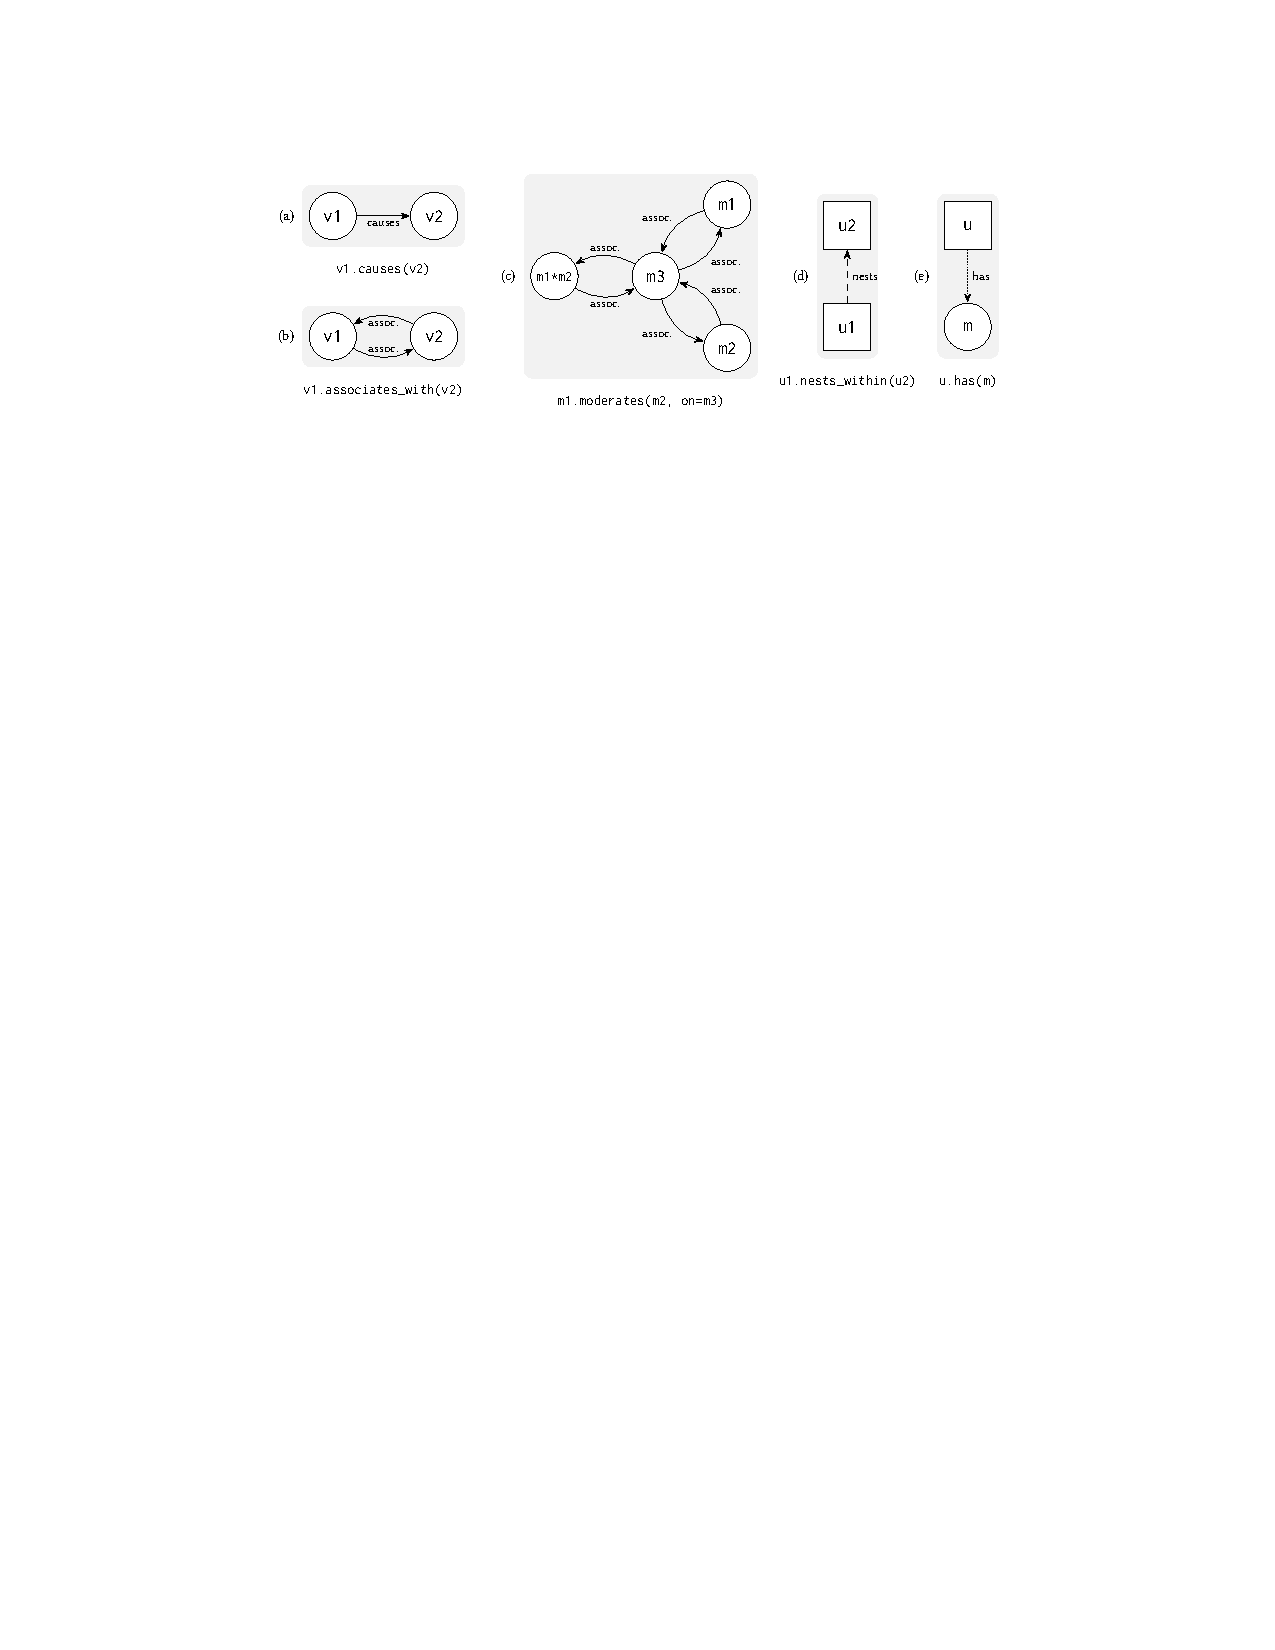
\includegraphics{tisane/figures/figure3}
%         \caption{Code snippets of conceptual and data measurement relationships written in Tisane's \SDSLlong and their representation in Tisane's graph IR. Variables are named with \texttt{u} for units, \texttt{m} for measures, and \texttt{v} for data variables that can be either units or measures. All edges depicted are those that are added due to the relationship. In the \texttt{moderates} example, we assume that \texttt{m1} and \texttt{m2} both belong to the same unit, and for simplicity, the attribution edge (labeled as ``has'') from \texttt{m1} and \texttt{m2}'s unit is not shown.}
%         \label{fig:figureSDSLToGraphIR}
%         \Description{Five directed graphs are shown. All nodes are labeled with a monospaced font. The first directed graph has two nodes, labeled “v1” and “v2”, both circles. There is a solid edge from “v1” to “v2” labeled “causes”. Below this graph is a code snippet reading “v1.causes(v2)”. The second directed graph also has two nodes, also labeled “v1” and “v2” and both circles. There are solid edges from “v1” to “v2” and from “v2” to “v1”. Both edges are labeled “assoc.” Below the graph is a code snippet: “v1.associates_with(v2)”. The third directed graph contains four nodes, which are labeled “m1*m2”, “m1”, “m2”, and “m3”. All are circles. There are six edges in the graph, all solid and labeled “assoc.” The edges are from “m1*m2” to “m3”, “m3” to “m1*m2”, “m1” to “m3”, “m3” to “m1”, “m2” to “m3”, and “m3” to “m2”. Below the graph is a code snippet: “m1.moderates(m2, on=m3)”. The fourth directed graph contains two nodes, labeled “u1” and “u2”. Both are squares. There is a dashed edge labeled “nests” from “u1” to “u2”. Below the graph is the code snippet “u1.nests_within(u2)”. The fifth, and final, directed graph contains two nodes labeled “u” and “m”. “u” is square-shaped and “m” is circle-shaped. There is a dotted edge from “u” to “m”, labeled “has”. Below the graph is the code snippet “u.has(m)”.}
%     \end{figure*}


\paragraph{Data measurement relationships.}\label{sec:data-measurement-relationships}

Study designs may have clusters of observations that need to be modeled explicitly for external validity.
For example, in a within-subjects experiment, participants provide multiple
observations for different conditions. An individual's observations may cluster
together due to a hidden latent variable. Such clustering may be imperceptible
during exploratory data visualization of a sample but can threaten external validity.
%(see~\ref{sec:validity}).
GLMMs can mitigate three common sources of clustering that
arise during data collection
~\cite{gelmanHill2006regression,kreft1998introducing,cohen1988statistical}:

\begin{itemize}
  \item \textbf{Hierarchies} arise when one observational/experimental unit
  (e.g., adult) nests within another observational/experimental unit (e.g.,
  group). This means that each instance of the nested unit belongs to one and
  only one nesting unit (many-to-one).
  % The nesting unit has multiple nested units.
  \item \textbf{Repeated measures} introduce clustering of observations from the
  same unit instance (e.g., participant).
  \item \textbf{Non-nesting composition} arises when overlapping attributes
  (e.g., stimuli, condition) describe the same observational/experimental unit
  (e.g., participant)~\cite{gelmanHill2006regression}.
\end{itemize}

The above sources of clustering pose three problems for analysts. First,
analysts must have significant statistical expertise to identify when data
observations cluster. Second, they must know how to mitigate these clusters in
their models. Third, with this knowledge, analysts must figure out how to
express these types of clustering in their analytical tools. Even if analysts
are not able to identify clustered observations, they are knowledgeable about
how data were collected.

% \enlargethispage{-12pt}

Thus, Tisane addresses the three problems by (i) eliciting data measurement
relationships from analysts to infer clusters and (ii) formulating the maximal
random effects structure, optimizing for external validity
(\ref{sec:interaction_model}). Below, we describe language features for expressing data measurement relationships.

\paragraph{Nesting relationships: Hierarchies}
\textbf{Hierarchies} arise when a unit (e.g., an \adult) is nested within another
unit (e.g., an exercise \group). Researchers may collect data with
hierarchies to study individual and group dynamics together or as a side effect of
recruitment strategies. To express such designs, Tisane provides the
\texttt{nests\_within} construct. Conceptually, nesting is strictly between
observational/experimental units, so Tisane type checks that the variables
that nest are both Units. %Tisane assumes there are multiple nested units within a nesting unit.
In the graph IR, a nesting relationship is encoded as an edge between two unit
nodes (\ref{fig:figureSDSLToGraphIR}(d)). There is one edge from the nested
unit (e.g., \adult) to the nesting unit (e.g., \group)~\footnote{The GitHub repo contains a gallery of examples that include nesting relationships.}.

\paragraph{Frequency of measures: Repeated measures, Non-nesting composition}
\def\numberofinstances{\texttt{number\_of\_instances}\xspace}
When a measure is declared through a unit, Tisane adds an
attribution edge (``has') from a unit node to a measure node (\ref{fig:figureSDSLToGraphIR}(e)).
A unit's measure can be taken one or more times in a study. The frequency of
measurement is useful for detecting repeated measures and non-nesting
composition. In \textbf{repeated measures} study designs, each unit provides
multiple values of a measure, which are distinguished by another variable,
usually time. \textbf{Non-nesting}~\cite{gelmanHill2006regression} composition
arises when measures describing the same unit overlap. For example, HCI researchers studying input devices might
design them to utilize different senses (e.g., touch, sight, sound).
Participants in the study may be exposed to multiple different devices, which
act as experimental conditions of senses. The conditions are intrinsically tied to the
devices, and participants can be described as having both conditions and
devices, which overlap with one another. Such study designs
introduce dependencies between observations~\cite{clark1973language} and hence
violate the assumption of independence that GLMs make.

\def\inputdevice{\texttt{device}\xspace} When analysts declare Measures, they
specify the frequency of the observation through the
\texttt{number\_of\_instances} parameter. This parameter accepts an integer,
variable, a Tisane \texttt{Exactly} operator, or a Tisane \texttt{AtMost}
operator. By default, the parameter is set to one. The \texttt{Exactly} operator
represents the exact number of times a unit has a measure. The \texttt{AtMost}
operator represents the maximum number of times a unit has a measure. Both
operators are useful for specifying that a measure's frequency depends on
another variable, which is expressible through the \texttt{per} function. For
example, participants may use two \inputdevice{}s \textit{per}
\texttt{condition} assigned: \texttt{device = subject.nominal(\upquote{Input
device}, number\_of\_instances=ts.Exactly(2).per(condition))}. \polish{Overruns column?} The \texttt{per}
function uses the Tisane variable's cardinality by default but can instead use a
data variable's \numberofinstances by specifying \texttt{use\_cardinality=False}
as a parameter to \texttt{per}. Moreover, specifying a measure's
\texttt{number\_of\_instances} to be an integer is syntactic sugar for using the
\texttt{Exactly} operator. Specifying a variable is syntactic sugar for
expressing \texttt{ts.Exactly(1).per(variable)}.

To determine the presence of repeated measures or non-nesting composition,
Tisane computes the \numberofinstances of measures and their relationship to
other measures. Measures that are declared with \numberofinstances equal to one
are considered to vary between-unit. Measures that are declared with
\numberofinstances greater than one or a variable with cardinality greater than
one are considered to vary within-unit as repeated measures. If there are
instances of a measure per another measure sharing the same unit, the measures
are non-nesting.

%     \begin{figure}[h]
% \centering
% 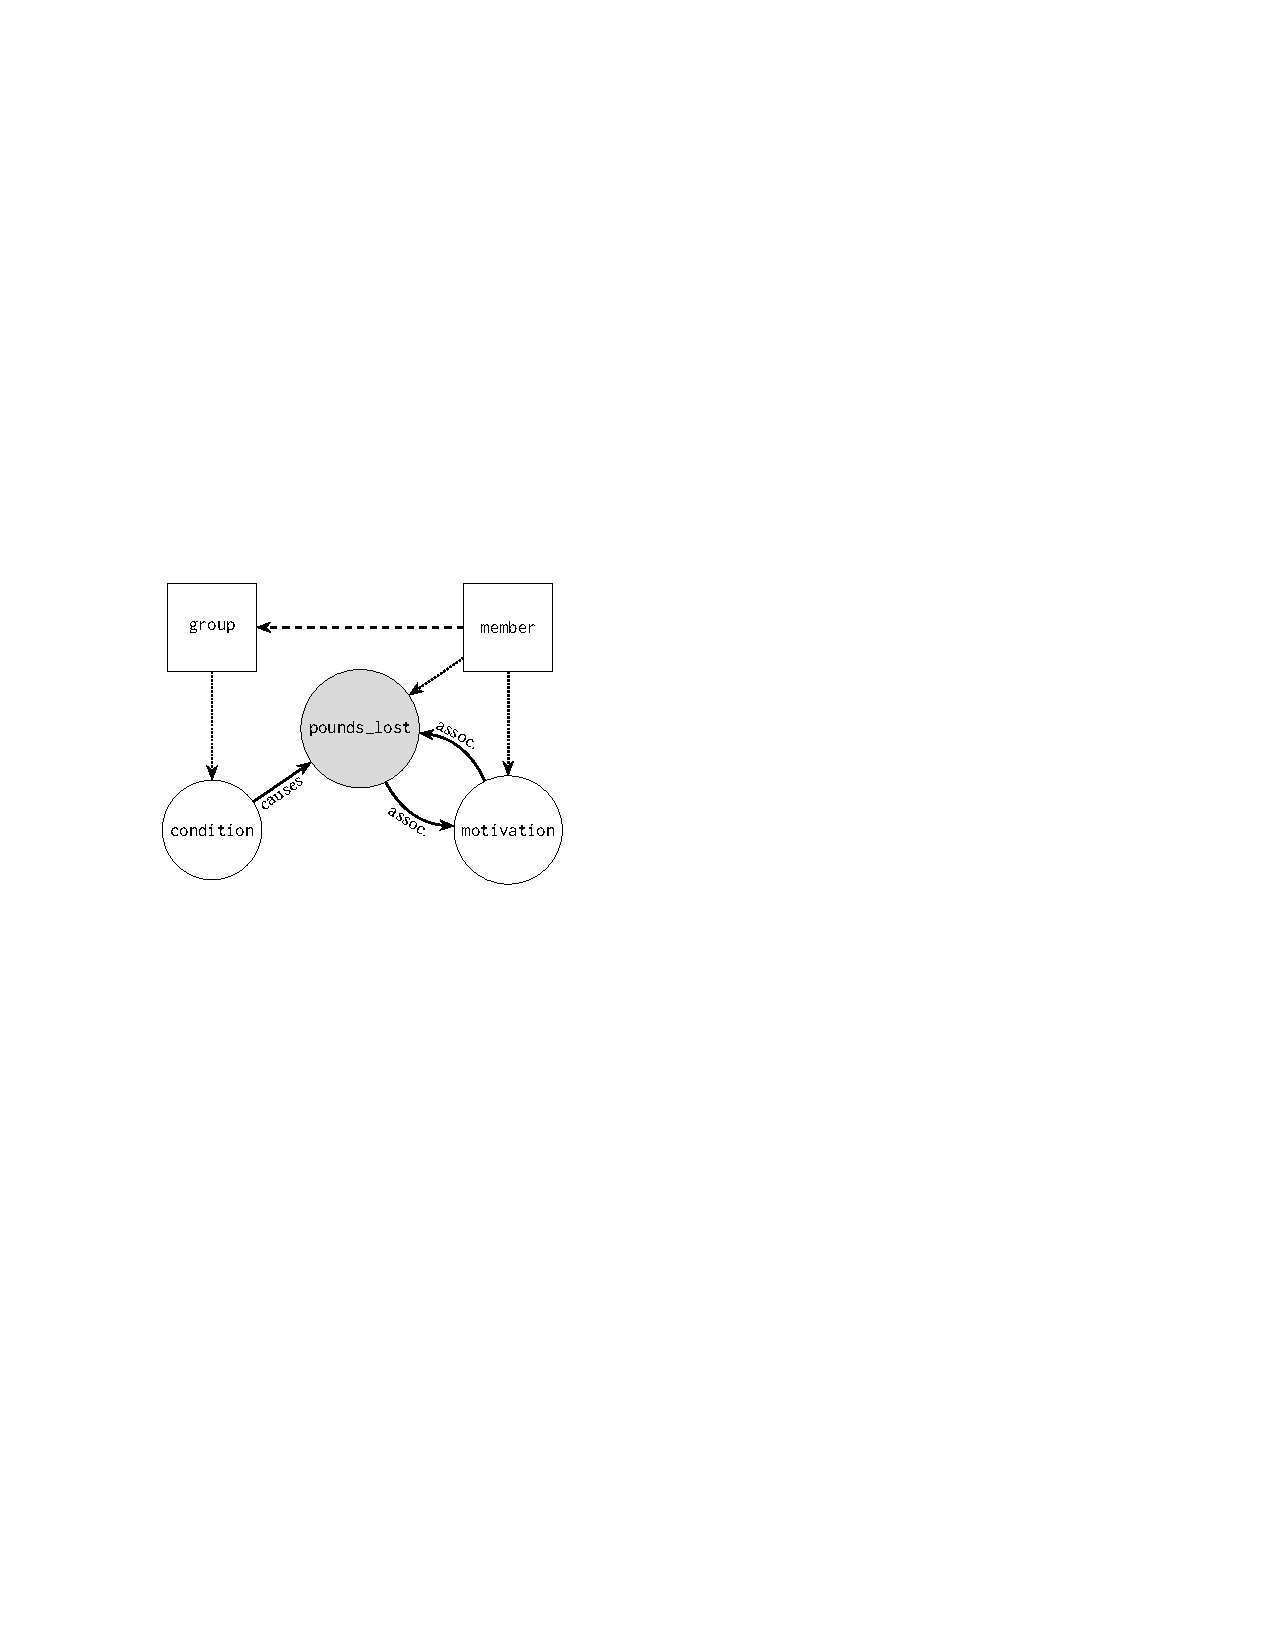
\includegraphics{tisane/figures/figure4}
%         \caption{The graph representation of the variables and relationships from the usage scenario. \texttt{causes} edges are labeled with ``causes''. \texttt{associates\_with} edges are labeled with ``assoc.'' Dashed edges indicate \texttt{nests\_within} relationships, and dotted edges indicate \texttt{has} relationships.}
%         \label{fig:figureGraphIRExample}
%         \Description{A directed graph of five nodes is depicted. The nodes are labeled “group”, “condition”, “pounds_lost”, “motivation”, and “member”, all in monospace font. The “group” node is square-shaped (indicating the node represents a Unit), and has a dotted edge pointing to the circle-shaped (indicating it's a Measure) “condition” node. The “condition” node has a solid edge labeled “causes” pointing to the circle-shaped, gray “pounds_lost” node. The gray color indicates that “pounds_lost” was the dependent variable. The “pounds_lost” node has one outgoing solid edge labeled “assoc.” (for associative relationships), to the circle-shaped node “motivation.” The “motivation” node has an outgoing, solid “assoc.” edges to the “pounds_lost” node. The final node, “member,” is square-shaped and has a dashed outgoing edge to the “group” node and dotted outgoing edges to the “pounds_lost” and “motivation” nodes. The dashed edge means “member” nests in “group” and the dotted edges mean that “pounds_lost” and “motivation” are measures of the “member” unit.}
%     \end{figure}

\subsection{Statistical model inference: Interactively querying the graph IR}
\label{sec:interaction_model} After specifying variable relationships, analysts
can query Tisane for a statistical model. Queries are constructed by specifying
a study design with a dependent variable (the value to be predicted) and a set
of independent variables (predictors). Tisane processes the query and generates
a statistical model in four phases: (1) preliminary conceptual checks that
validate the study design, (2) inference of possible effects structures and
family and link functions, (3) input elicitation to disambiguate possible
models, and (4) generation of a final executable script, and a record of decisions during disambiguation. Given that the interactive process begins with
an input program using Tisane and outputs a script for fitting a GLM or GLMM, we
call this process \textit{interactive compilation}.

\subsubsection{Preliminary checks} \label{sec:prelim-checks}
At the beginning of processing a query, Tisane checks that every input study
design is well-formed. This involves two conceptual correctness checks. First,
every independent variable (IV) in the study design must either cause or be
associated with the dependent variable (DV) directly or transitively. Second, the
DV must not cause any of the
IVs, since it would be conceptually invalid to explain a
cause from any of its effects. If any of the above checks fail, Tisane
issues a warning and halts execution. By using these two checks, the Tisane
compiler avoids technically correct statistical models that have little to no
conceptual grounding (\dcConceptualKnowledge). If the checks pass, Tisane proceeds to the next phase.
% Tisane ensures that any statistical model it infers is both conceptually and
%technically valid relative to the analyst's specified relationships.

\subsubsection{Candidate statistical model generation}
A GLM/GLMM is comprised of a model effects structure, family function, and link
function. The model effects structure may consist of main, interaction, and
random effects. Tisane utilizes variables' conceptual relationships to infer candidate
main and interaction effects and data measurement relationships to infer
random effects. Tisane infers family and link functions based on the data type
of the DV in the query. The candidate statistical models that Tisane
generates, based on the graph and query, seed an interactive disambiguation
process.

The purpose of identifying candidate main effects beyond the ones analysts may
have specified is to provoke consideration of erroneously omitted variables that
are conceptually relevant and pre-empt potential confounding and
multicollinearity issues that may arise.

\paragraph{Deriving Candidate Main Effects}
In a query to infer a statistical model, analysts specify a single dependent
variable and a set of one or more IVs. After passing the checks described in~\ref{sec:prelim-checks}, %As described above, the input IVs are
%checked to make sure that they have conceptually causal or associative %relationships. %Given that they do,
the query's independent variables are considered candidates. In addition, Tisane
derives three additional sets of candidate main effects intended to control for
confounding variables in the output statistical model\footnote{Tisane currently
treats each input IV as a separate ``exposure'' variable for which to identify
confounders. Tisane then combines all confounders into one statistical model.}.
The first two sets below are from the ``modified disjunctive cause
criterion''~\cite{vanderweele2019modifiedDisjunctiveCriterion}:

\begin{itemize}    
    \item \textbf{Causal parents.} For each IV in the query, Tisane finds its
    causal parents (see~\ref{fig:figureCandidateMainEffects}(a)).
    % , as recommended
    % by~\cite{vanderweele2019modifiedDisjunctiveCriterion}.
    \item \textbf{Possible causal omissions.} Tisane looks to see if any other
    variables not included as IVs cause the DV 
    % , as recommended
    % in~\cite{vanderweele2019modifiedDisjunctiveCriterion} 
    (see
    in~\ref{fig:figureCandidateMainEffects}(b)). They are relevant to the DV
    but may have been erroneously omitted.
    \item \textbf{Possible confounding associations.} For each IV, Tisane looks
    for variables that are associated with both the IV and the DV (see
    in~\ref{fig:figureCandidateMainEffects}(c)). Because associations
    between variables can have multiple underlying causal structures, Tisane
    recommends variables with associative relationships with caution. Tisane
    issues a warning describing when not to include such a variable in the GUI.
\end{itemize}

\figureCandidateMainEffects

%     \begin{figure*}%[h]
% \centering
% 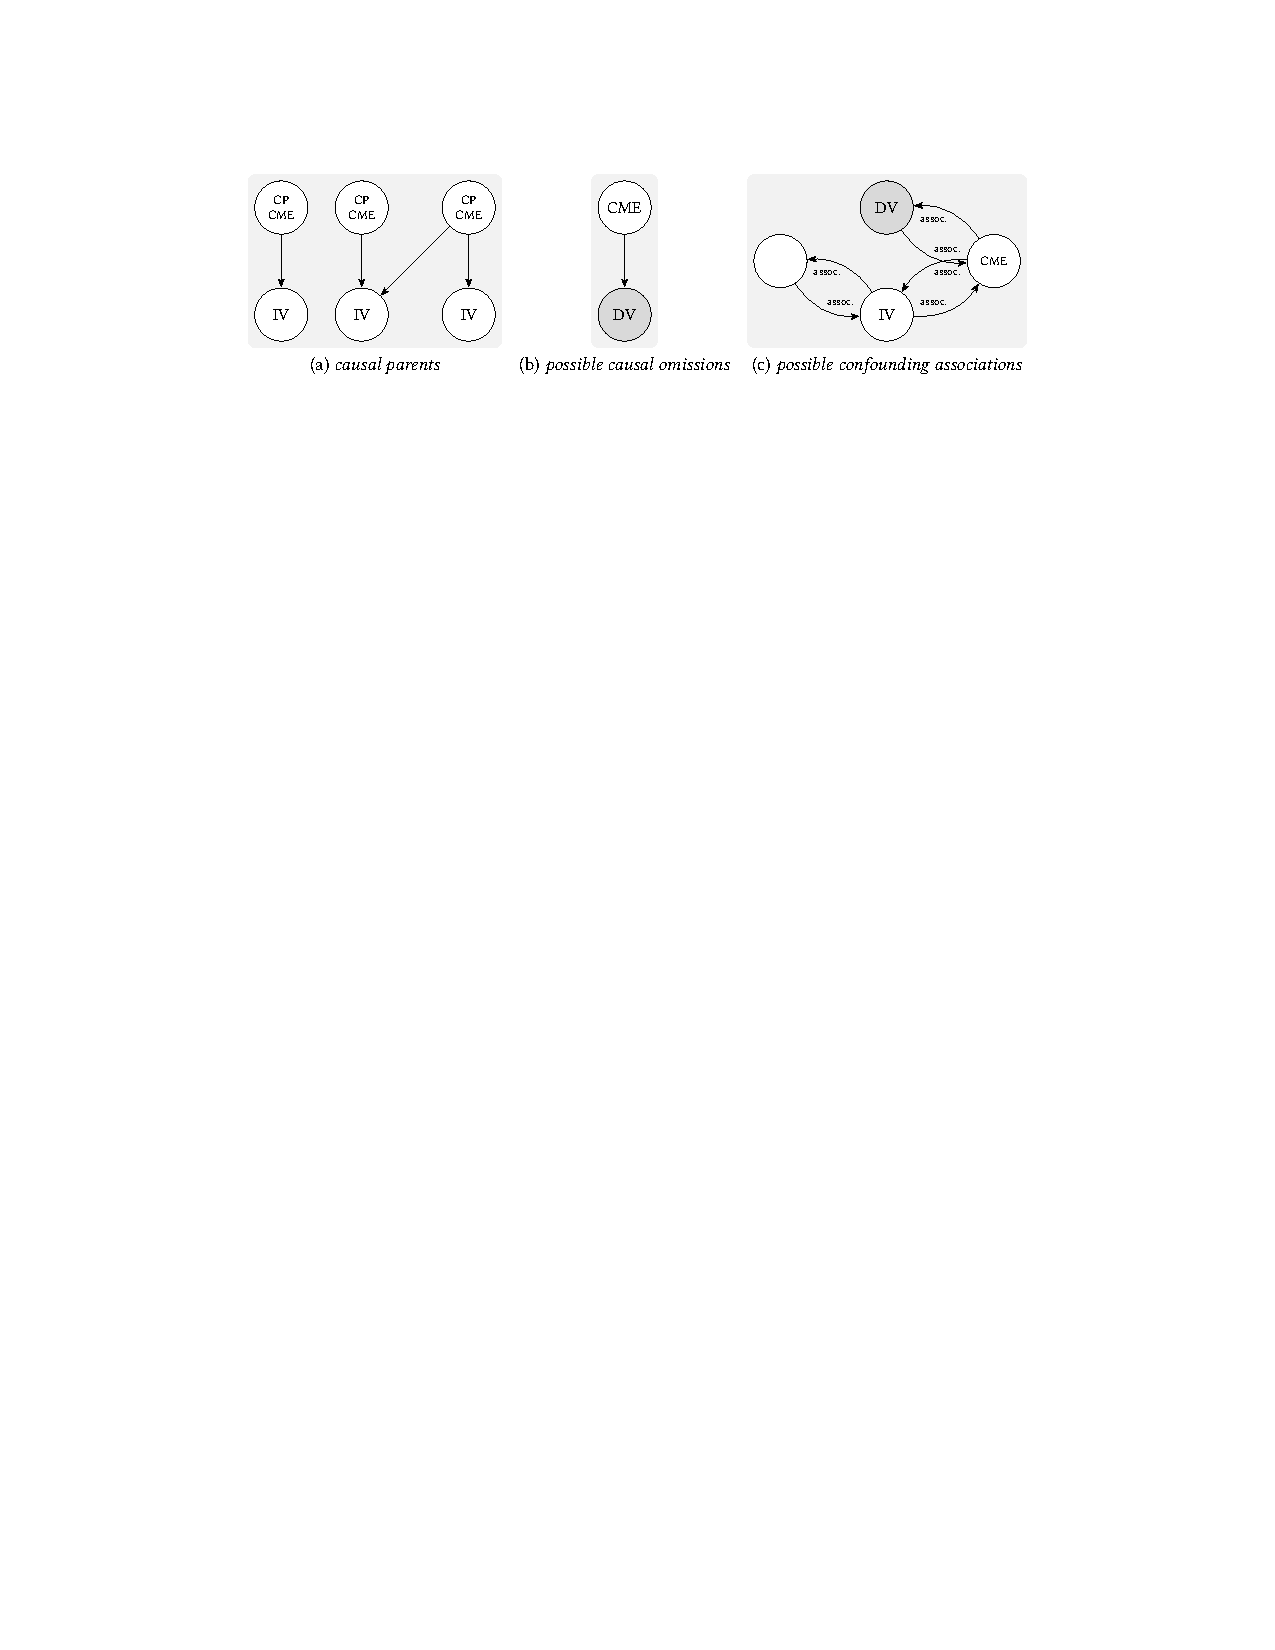
\includegraphics{tisane/figures/figure5}
%         \caption{Graphs demonstrating causal parents, possible causal omissions, and possible confounding associations. In graphs (a) and (b) (left and middle), all edges are causal. Independent variables are marked ``IV'', discovered candidate main effects ``CME'', dependent variables ``DV'', and causal parents ``CP''.}
%         \label{fig:figureCandidateMainEffects}
%     \end{figure*}

Using the above rules, Tisane suggests a set of variables that are likely
confounders of the variables of interest expressed in the query. There may be
additional confounders due to unmeasured or unexpressed variables that are either
not known or excluded from the graph. Tisane never automatically includes the
candidate main effects in the output statistical model. Analysts must always
specify a variable as an IV in the query or accept a suggestion (\dcGuidance).

If a graph only contains associates edges then the candidate main effects Tisane
suggests are those that are directly associated with both the DV and an IV. If a
graph has only causal edges, Tisane would suggest variables that directly cause
the DV but were omitted from the query and the causal parents of IVs in case the
parents exert causal influence on the DV through the IV or another variable that is not
specified.

The total set of main effects, including variables the analyst has specified as
IVs in their query and candidate main effects, are used to derive candidate interaction
effects and random effects, which we discuss next.

% However, relying on formal causal analysis to guide modeling is insufficient,
% and additional methods for ensuring conceptual validity are necessary.
\paragraph{Deriving Candidate Interaction Effects}
An interaction between variables means that the effect of one variable (the \textit{moderated} variable) on a \textit{target} variable is moderated by another (non-empty) set of variables (the \textit{moderating} variables). Tisane's
\SDSL already provides a primitive, \texttt{moderates}, to
express interactions. As such, Tisane's goal in suggesting candidate interaction
effects is to help analysts avoid omissions of conceptual relationships
that are pertinent to an analyst's research questions or hypotheses (\dcConceptualKnowledge).
Candidate interaction effects are the interaction nodes whose (i) moderated and moderating variables include two or more candidate main effects and (ii)
    target variable is the query's DV.

\paragraph{Deriving Candidate Random Effects} \label{sec:deriveRandomEffects}
Random effects occur when there are clusters in the data, which occur when
we have repeated measures,
nested hierarchies, or non-nesting composition (as defined in subsection~\ref{sec:data-measurement-relationships}). Tisane implements Barr et al.'s recommendations
for specifying the maximal random effects structure of linear mixed effects
models for increasing the generalizability of statistical
results~\cite{barr2013random, barr2013randomUpdated}.

To derive random effects, Tisane focuses on the data measurement edges in the
graph IR. Using the graph IR, Tisane identifies unit nodes, looks for any nesting
edges among them, and determines within- or between-subjects
measures based on the frequency of observations for units. % by using metadata stored in the attribution edges about the number of
%observations each unit has of any particular measure.
From these, Tisane
generates random intercepts of units for the unit's measures that are between-subjects as well as the unit's measures that are within-subjects where each instance of the unit
has only one observation per value of another variable. Tisane generates random slopes of a unit and its measure for all measures
that are within-subjects where each instance of the unit has multiple
observations per value of another variable. For interaction effects, random
slopes are included for the largest subset of within-subjects variables (see~\cite{barr2013randomUpdated}). %,
%according to Barr's updated recommendations~\cite{barr2013randomUpdated}.
Tisane handles correlation of random slopes and intercepts during disambiguation (subsection~\ref{sec:disambiguation}).
%When there are both random slopes and random intercepts for the same unit, Tisane asks analysts if they are correlated during disambiguation. By default, Tisane assumes correlation.
% due to computational limitations or insufficient data,
Maximal random effects may lead to model convergence issues that analysts
address by later removing or adding independent variables and random effects. Nevertheless, starting with
a maximal, valid model is important for ensuring that future revisions are also valid (\dcValidity).

\paragraph{Deriving Candidate Family and Link Functions} \label{sec:family_link_functions}
The DV's data type determines the set of candidate family and
link functions. For example, numeric % or continuous data
variables cannot have
binomial or multinomial distributions. Similarly, nominal variables are not
allowed to have Gaussian distributions. Furthermore, each family has a set of
possible link functions. For example, a Gaussian family distribution may have an
Identity, Log, or Square Root link function. The statistics literature documents
    possible combinations of family and link functions for specific data
types~\cite{nelder1972generalized}.
%  that software tools such as
% statsmodels~\cite{statsmodelsRef} and lme4~\cite{bates2014fittingLme4}
% implement.

Tisane includes common family distributions as candidate families and their
applicable link functions. In its current implementation, Tisane relies on
\statsmodels~\cite{statsmodelsPaper} for GLMs and
\texttt{pymer4}~\cite{jolly2018pymer4} for GLMMs. As such, Tisane is limited to
the family and link function pairings implemented in these
libraries.~\autoref{tab:tableFamilyLinkFunctions} lists the family and link
functions these libraries currently supports. As \statsmodels' and \pymer's
support for GLMs grows in the future, Tisane can be extended.
% Tisane can be
% extended to take advantage of new family and link implementations in these
% libraries.

\tableFamilyLinkFunctions

\subsubsection{Eliciting Analyst Input for \Disambiguation}\label{sec:disambiguation}
\groupExerciseDisambiguation
% Upon generating a set of candidate main, interaction, and random effects, Tisane
% asks analysts questions before outputting a statistical model.
The disambiguation process provides an opportunity for analysts to explore the
space of generated models based on their original query. Given our design
considerations to prioritize conceptual knowledge (\dcConceptualKnowledge) and
give analysts guidance (\dcGuidance), we designed a GUI to scaffold analysts' reasoning and elicit their input.
For versatility, we implemented Tisane's GUI using Plotly
Dash~\cite{plotlyDash}. Analysts can either execute their Tisane programs and use the
GUI inside a Jupyter notebook (no additional widgets needed) or run
their Tisane programs in an IDE or terminal, in which case Tisane will open the
GUI in a web browser. 
% Figure~\ref{fig:groupExerciseDisambiguation}
% gives an overview of the GUI.

% Tisane grounds explanations and disambiguation questions in the
% variable relationships analysts declared in their input Tisane program,
% for explaining why specific generated main and interaction effects may be
% desirable, how Tisane automatically inferred the random effects structure, and
% show data distributions to help analysts select family and link functions (Figure~\ref{fig:groupExerciseDisambiguation}).
Candidate statistical models are organized according to (i) independent
variables  (main effects and interaction effects), (ii) data clustering (random
effects), and (iii) data distribution (family and link functions). In the main
effects tab, Tisane asks analysts if they would like to include additional or
substitute main effects that Tisane infers to be conceptually relevant. In the
interaction effects tab, Tisane suggests moderating relationships to include but
does not automatically include them because analysts may not have specific
hypotheses involving interactions (\dcGuidance). If analysts do not specify any
moderating relationships, Tisane does not suggest any interaction effects,
preventing analysts from including arbitrary interactions that may be
conceptually unfounded (\dcConceptualKnowledge, \dcValidity).

In the data clustering tab, Tisane shows analysts which random effects it
automatically includes based on the selected main and interaction effects. Unlike
main and interaction effects, Tisane automatically includes random effects
in order to maximize model generalizability (\dcValidity). If there is a random
slope and random intercept pertaining to the same unit, Tisane asks analysts if
they should be correlated or uncorrelated. We provide this option because
analysts may have relevant domain expertise to make this decision (\dcGuidance).
By default, Tisane correlates the random slope and random intercept.

The final tab, data distribution, helps analysts examine their data and select
an initial family and link function to try. Appropriate selection of family and
link functions depends on the data type of the dependent variable and the
distribution of model residuals. Therefore, the selection can only be assessed
after choosing a family and link function in the first place.

For an initial statistical model to consider, Tisane narrows the set of family
functions considered based on the declared data type of variables
(see~\ref{sec:family_link_functions}) and lightweight viability checks, such
as ensuring that a Poisson distribution is only applicable for variables that
have nonnegative integer values. Tisane asks questions designed to uncover
more semantically meaningful data types (e.g., counts) than are provided at
variable declaration. Analysts without data can answer these questions as they
are planning their studies (\dcStatisticalPlanning). For the selected family
candidate, Tisane automatically selects the default link function based on the
defaults for \statsmodels~\cite{statsmodelsRef} and
\texttt{pymer4}~\cite{jolly2018pymer4}. Analysts can then choose a different
link function, as long as it is supported.
% \footnote{See supplemental material for
% a complete listing of Tisane's supported family and link function pairings.}.}
% We chose to ask these questions during
% disambiguation rather than provide additional data types to Tisane's \SDSL to
% simplify the variable declaration process. \ej{Not sure I believe this.}}

\subsubsection{Output}
There are two outputs of the interactive compilation: (ii) an executable modeling script and (ii) a log of GUI
choices. To increase transparency of the
authoring process, Tisane provides a log of user selections in the GUI as
documentation, which the analyst can include in pre-registrations, for example
(\dcStatisticalPlanning). In the output script, Tisane includes code to fit the
model and plot residuals against fitted values in order to assess the
appropriateness of family and link functions, as is typical when examining
family and link functions. The output script also includes a comment explaining
what to look for in the plots and an online resource for further reading. Should
analysts revise their choice of family and link functions, they can re-generate
a script through the Tisane GUI.

% \section{Initial Evaluation: Case studies with real-world researchers}
\section{Initial evaluation: Case studies with researchers}\label{sec:tisane_case_studies}
Given Tisane's novel focus on deriving and
guiding analysts toward valid statistical models, we assessed how Tisane affects
data analysis practices in three case studies with researchers. The following research questions guided
the evaluation:
\begin{itemize}
    \item \rqWorkflow How does Tisane's programming and interaction model
    affect how analysts author models? Specifically, what does Tisane make
    noticeably easier or more difficult when conducting an analysis?
    %Where do researchers find themselves spending more time or attention
    %compared to without Tisane? % What are you doing? not doing?
    \item \rqCognitive Where do researchers report spending more
    time or attention when using Tisane? How does this compare to their
    fixation during analyses typically?
    \item \rqFuture When do researchers imagine using Tisane
    in future projects, if at all? What additional support do researchers want
    from Tisane? 
\end{itemize}

We recruited researchers through internal message boards and individual
contacts. We intentionally recruited researchers at different stages of the
research process---study planning, data analysis for publication, and ongoing
model building and maintenance. We believed this could help us more holistically
evaluate Tisane's impact on data analysis. We met with researchers over Zoom
[R1, R3] and in person [R2] to discuss their use cases, observe them use
Tisane for the first time, and ask for open-ended feedback. We pointed researchers to the Tisane tutorial for
installation instructions and examples but otherwise encouraged the researchers
to work independently. We answered any questions researchers had while using Tisane.
Each study session lasted approximately 2 hours. At the end, two of the three
researchers [R1, R3] said they planned to use Tisane again over the next two months.

\subsection{Case Study 1: Planning a New Study}
R1, a clinical psychology PhD student, had recently submitted a paper and was
planning a follow-up.
% to ask based on knowing how to author models she
% understood conceptually but had low confidence specifying correctly on her
% own.
R1 reported that she had never taken a formal class on modeling techniques but
taught herself for her last paper. Her general workflow involved consulting with
and mirroring what others in her research group did even if she did not
completely understand why. R1 did not program often but said she had ``enough
coding experience to understand this kind of...[sample program].'' Although
familiar with Python, R1 preferred M+~\cite{mplus} and SPSS~\cite{spss}. She was
interested in using Tisane to brainstorm new studies and research questions.

\textit{Using Tisane.} After installation, R1 read through one of the
computational notebook examples available in the Tisane GitHub repository.
While reading, R1 asked clarifying questions about the variable types and
syntax. R1 explained that the \texttt{Design} class felt novel because she had
never seen the concept of a study design in data analysis code before. When the
first two authors explained that it was supposed to be the equivalent of the
statement of a study design in a paper, R1 remarked that usually, she ``[kept]
that in [her] head, which [she] probably shouldn't'' (\rqCognitive). Without
a concrete data set, R1 preferred to walk through more examples %and discuss how
%their Tisane program would differ
rather than author a script of her own.

While reading an example, R1 drew a parallel between the tabs in SPSS dialogs for specifying models and
the tabs in the Tisane GUI, noting that SPSS had a tab for control variables.
R1 also wanted the ability to distinguish between ``control
variables'' and other independent variables in the Tisane GUI. R1 explained that this
would map more closely to how psychologists think about analyses.
Future work could incorporate additional language constructs, such as
a new data type for controls, for different groups of users (\rqFuture).
% This feedback
% suggests that future work could examine additional language constructs, such as
% a new data type for controls, would be helpful for different groups of users (\rqFuture).

\begin{comment}
R1 explained how in the past, she had run a series of tests only to learn later
that she should have been using GLMs. Even when she constructed the GLMs, %linear models,
she expressed uncertainty about her choice of family function: ``I don't know
[what] I was exactly picking...like Poisson regression or whatever.''
% ...I honestly, admittedly did not really look into which I should have been picking...but I just had one of [a colleague's] previous students [say],
R1 explained that she was given little guidance on choosing a model; another
student just told her, ```This is what I did. So you should just do that.''' In
contrast, R1 really liked having the normality checks and data histograms
available in the Tisane GUI to be more aware of the data (\rqCognitive).
\end{comment}

At the end of the study session, R1 remarked how Tisane ``fills in a lot of
the...gaps'' in data analysis (\rqWorkflow, \rqCognitive). The first gap R1
discussed was the \emph{programming gap} between scientists and statistical
tools. R1 believed that, for scientists who were not comfortable with
programming, ``they should probably be running less complex models, or first
learn how to code'' even if the complex models would be most appropriate. The
second gap R1 discussed was the \emph{statistical knowledge gap} in tools. R1 explained that
in her experience, R provides support for more complex models but little
guidance for what those models or statistical tests should be, requiring ``top
down assumption[s].'' Thus, to R1, Tisane bridged the gap between tools like
SPSS and R by requiring minimal programming and providing modeling support. Put
another way, Tisane bridged the gulf of execution~\cite{norman2013doet} for R1
that previous tools had not.
% conflation of programmign and analysis skills, making it easier for people to
% author models who may not be programmers yet need to for their work/research

% R1
% mentioned that in clinical psychology, it is often not possible to find causal
% relationships, and was more interested in finding novel correlations in the data.
% R1 was at the planning stage of data analysis, and was


\subsection{Case Study 2: Analyzing Data for a Paper Submission}
% \textit{Analysis task.}
R2, a computer science PhD student, had conducted a within-subjects study where
47 participants used four versions of an app for one week each (four
weeks total). The motivating research question was how the different app designs
led to %levels of
psychological dissociation. % during usage.
% R2 had logged
% self-report survey responses, click behavior, and time spent in %on specific elements of
% the app.
Although R2 had expected to collect multiple survey responses for each
participant each day, they only had
aggregate daily self-report measures due to an error in the database management system.
% As a result, R2 was
% unsure about which models to use for the aggregated ordinal
% data. % and which models to use.
%Using lecture notes from a past statistics course,
In the past, R2 reported having extensively explored their data and
consulting others, but for this paper, they had not explored their data prior to
fitting models because they felt more confident in their modeling skills. For
analyses, R2 preferred R but had general Python programming experience. Prior
to using Tisane, R2 had authored linear mixed effects models in R for their
study. They were interested in using Tisane to check their analyses prior to
submitting their paper to CHI.


\def\numberofinstances{\texttt{number\_of\_instances}\xspace}


\textit{Using Tisane.} %R2
%wrote two scripts using Tisane over the course of two hours.
R2 wrote their scripts by adapting an
example from the Tisane GitHub repository.
% While authoring
% their scripts, R2 read the API documentation and examples closely and found
% \texttt{SetUp} variables novel but understandable.
% After a brief explanation, R2 specified date of study to be a \texttt{SetUp} variable.
As R2 considered which conceptual relationships to add, they reasoned aloud about
if they should state causal or associative relationships between various measures and dissociation (\rqCognitive). % R2 found stating conceptual relationships difficult, stating:
%On one hand, ``[a participant] taking [one of the recorded
%actions] [does not spark] dissociation for them,'' but on the other hand,
%``dissociation might be causing them to...take that action.'' 
After some
deliberation, they said, ``I don't feel comfortable [making a causal
statement],'' and instead specified \texttt{associates\_with} relationships.
R1's hesitation to assert causal relationships confirms prior findings that
specifying formal causal graphs is difficult for domain
researchers~\cite{suzuki2020causal,suzuki2018mechanisms,velentgas2013developing} and our design choice
to allow for association edges.
% ``Because...for instance, if people use like a dialog exit to leave an app, that doesn't...cause them to dissociation...them taking that action is not sparking dissociation for them, but...dissociation might be causing them to...take that action....I don't feel comfortable [making a causal statement]. We can just say it's associated.''
In addition, R2 was initially unsure about how to specify the
\numberofinstances for their measures since their original study design
was unbalanced. %Participants could have varying numbers of measures logged per day.
After asking for clarification about \numberofinstances,
R2 declared all the measures with the parameter
\numberofinstances set equal to \texttt{date}.
% Given that they had decided to aggregate measures for each day for each
% participant,
% R2 reasoned that they could specify the measures to repeat once for
% each day in the study by declaring all the measures with the parameter
% \numberofinstances set equal to \texttt{date}.

Next, R2 ran their script %from the terminal
and used the Tisane GUI in a browser window. Based on Tisane's recommended
family and link functions, R2 realized the models they had previously authored
in R using a Gaussian family were inappropriate. Due to a bug that we have since
fixed, Tisane suggested a Poisson family that R2 used to generate a script, but
this was an invalid choice given that not all dependent variable values were
nonnegative integers. R2 explored other family distributions and generated a new
script using an Inverse Gaussian family. When executed, the second output script
issued an error due to the model inference algorithm failing to converge.
R2 made a note to look into this model further on their own.

\begin{comment}
Based on Tisane's reported normality test
results, they realized they could not assume their data were normally
distributed and that using a linear mixed effects model was inappropriate.
Although exploratory data analysis (EDA) would have led to the same insight, R2
said they had skipped EDA. %visualizing
%their data
%before fitting models.
As such, Tisane could help researchers %like R2
familiarize themselves with data and return to EDA (\rqWorkflow, \rqCognitive).
Upon seeing the histogram of their data overlaid with simulated data, R2
initially picked the Poisson family and executed Tisane's output script, but R2
received a model fitting error because not all dependent variable values were
nonnegative integers. We have since implemented an additional check to ensure
that Poisson is a choice only when all dependent variable values are nonnegative
integers.
% (since they were averages). Realizing that a Poisson model was inappropriate,
R2 explored the other family distributions and generated a new script using an
Inverse Gaussian family. The new output script issued an error due to the model
inference algorithm failing to converge. R2 made a note
%in their R Markdown file
to look into Inverse Gaussian distributions. %The analyst experienced similar issues for their second dataset and script.
%In the past, R2 had tried every single model, even picking one they
%had never heard of before
\end{comment}

Once finished using Tisane, R2 commented that their analysis with Tisane was more streamlined (\rqWorkflow) in contrast
to their very first paper where they had tried ``every
single kind of model that [they] could'' until finding ``the one that fits best,''
%This is the one I'm gonna use.' And I had to explain why I was using it because it was like
even if it was ``one that no one would have heard of.''
R2 also stated they would be interested in using Tisane earlier
in their analysis process in the future (\rqFuture).
%In addition, they reported being more focused on ``<fill in.>`` %(\textit{cognitive impact}).
Based on their experience with Tisane, R2 questioned their previously authored linear mixed effects model, and said it was ``unnerving'' to
discover an issue so close to a deadline. At the same time, they expressed, ``if it's incorrect, I should know
before I submit.'' A day after the study, R2 contacted the authors to inform them that they had decided to
update their analyses from linear mixed effects models to generalized linear
mixed effects models. They reported using the Inverse
Gaussian family after visualizing and checking the distribution of residuals
with help from the output Tisane script. The Inverse Gaussian family was
appropriate because their dependent variable's values were all nonnegative and
displayed a slight positive skew.
% R2 was still in the process of re-analyzing
% their second dataset.
R2's experience with Tisane suggests that Tisane can help
researchers catch errors and lead them to re-examine their data, assumptions,
and conclusions.

\subsection{Case Study 3: Developing Models to Inform Future Models}
Employed on a research team, R3 analyzes health data at the county, state,
and national levels to estimate health expenditure and inform public policy. R3
develops initial models that are used to validate and generate estimates for
larger, more comprehensive models.
% using a minimal set of covariates that will not be included in the final models was a primary concern.
Due to the
scale of data and established collaborative workflows, R3 typically works in a
terminal or RStudio through a computing cluster and had very little experience
with Python. Despite working on statistical models every day, R3 described himself as
``not...a great modeler.''
% He also appeared to be the most experienced R user among the
% researchers in our pilot and case studies.
R3 was interested in using Tisane to
determine what variables to include as random effects in a model.
% He had a limited number of variables to include in his model.

\def\statename{\texttt{state\_name}\xspace}
\def\yearid{\texttt{year\_id}\xspace}
\def\cardinality{\texttt{cardinality}\xspace}

\textit{Using Tisane.} R3 used Tisane in a local Jupyter notebook as well as on
his team's cluster. R3 used the Tisane API overview reference material on GitHub
to start writing his program, which involved copying and pasting the functions
with their type signatures and then modifying them to match his dataset and
incrementally running the program. The most common mistake R3 made while
authoring his Tisane program was to refer to variables using the string names in
the dataset (e.g., \texttt{"year"}) instead of the variable's alias (e.g.,
\yearid), an idiom common in R but not in Python.

While authoring his Tisane program, R3 found the \numberofinstances parameter
redundant, especially because his data is always ``square.'' Every \statename\
in his data set had 30 rows of data, corresponding to the \yearid{}s 1990-2019.
This is in contrast to R2, whose study design was unbalanced and resulted in
variable numbers of observations per participant that needed to be aggregated. Based on R3's feedback, we
added functionality to infer \numberofinstances for each unit, which analysts can inspect by
printing the variable.

% that's a statistical lack of knowledge on my hand, the fact that it's not normal. I don't know what to do with it.
While giving open-ended feedback on Tisane, R3, similar to R1, liked how Tisane helped ``fill
[the] gap in...[his] knowledge'' (\rqCognitive). Given the diversity of models
R3 works with, R3 found Tisane's focus on GLMs and GLMMs a ``little limiting'' and also
wished to make Tisane ``run without...the mouse'' in a script, as is typical in
his workflow (\rqWorkflow). Specifically, R3 described how he and his
collaborators typically want to explore a space of models and run them in
parallel. Nevertheless, R3 foresaw using Tisane in three types of modeling tasks
common in his work: (i) exploratory modeling to determine if there are any
interesting relationships between variables, (ii) authoring and comparing
multiple models for prediction, and (iii) working out the precise model
specification after identifying variables of interest (\rqFuture).

\subsubsection{System changes and Takeaways}
%However, given that (i) violations to normality assumptions may be acceptable with large enough sample sizes, 

We fixed bugs and iterated on Tisane's GUI based on feedback from
researchers. The largest change we made was to the data distributions tab. The data distributions
tab we tested with researchers visualized the dependent variables
against simulated distributions of family functions and included the results of the Shapiro-Wilk and D'Agostino and Pearson's normality tests. All three researchers
reported becoming more aware of their data due to the visualizations. However, researchers' enthusiasm for the feature made us wary that visualizing the simulated data 
could mislead less careful analysts to believe that family and link functions pertain to variable
distributions rather than the distributions of the model's residuals. 
To avoid
such errors while still helping analysts become more aware of their data, we
removed the simulated visualizations and normality tests and instead provide questions about the semantic nature of the dependent variable
% data
collected, as discussed in~\autoref{sec:disambiguation}.

Overall, Tisane streamlines the analysis process (\rqWorkflow) in part because
researchers report formalizing their conceptual knowledge into statistical
models more directly [R1, R2]. Although Tisane does not eliminate the need for
model revision, Tisane may scope the revisions analysts consider to significant
issues instead of details that may detract from the analysis goals [R2].
Additionally, researchers reported a perceived shift in their attention from
keeping track of and analyzing all possible modeling paths to their research
questions and data assumptions (\rqCognitive) while planning a new study and
analysis [R1] as well as while preparing a research manuscript [R2]. Future
adoption of Tisane may depend on the complexity of analyses (\rqFuture) [R3].
For instance, Tisane may provide a streamlined alternative to false starts due
to misspecifications for simpler analyses [R1, R2, R3]. For more complex models
and studies, Tisane may act more as a prototyping tool for statistical models,
helping researchers start at a reasonable model that they can then revise [R2,
R3]. Regardless of analysis complexity, externalizing analysts' conceptual
models in \tisane enhances documentation and communication of science,
potentially by enriching preregistered studies and analyses.

\section{Limitations and Motivation for Re-design}
While overall positive, the case studies made us aware of confusing keywords and
language constructs in \tisane. In order to improve \tisane and probe more
closely into what challenges statistical novices face when expressing their
domain knowledge, we engaged in an iterative process to re-design \tisane. We
started with a lab study using \tisane~\cite{jun2022tisane} to elicit
statistical non-experts' implicit definitions and assumptions about Tisane's
keywords and identify opportunities to refine \tisane's DSL and interactivity.

% . Observations from this study gave us ideas for
% re-designing Tisane's \SDSL. 

% Surprisingly, we found that some
% keywords and functions in \tisane were at too high a level of abstraction.
% Analysts wanted to express their conceptual relationships with greater detail
% and specificity. Analysts also wanted to express ambiguity about the a
% relationship's direction in the conceptual model. 


\section{Summary of Contributions}

% Reminder: Thesis statement
% Domain-specific languages that provide abstractions for expressing conceptual
% knowledge, data collection procedures, and analysis intents instead of specific
% statistical modeling decisions coupled with automated reasoning to compile
% conceptual specifications into statistical analysis code help statistical
% non-experts more readily author valid analyses. 

\tisane embodies the hypothesis central to this dissertation: A DSL for
expressing implicit conceptual knowledge and automated reasoning enable
statistical non-experts to author valid statistical models. In case studies of
\tisane, we found that the DSL (\thesisChallengeExplicit) makes analysts more aware of
their implicit domain knowledge. By deriving statistical models from
externalized conceptual models (\thesisChallengeRep), \tisane also fills in the
statistical knowledge and programming gaps analysts face when authoring
statistical analyses. \tisane demonstrates how these two approaches combined,
can improve statistical model authoring for statistical non-experts. 

% evidence for how
% connecting conceptual modeling to statistical modeling increases the statistical
% conclusion and external validity of analyses~\cite{shadish2010campbell}.  

% The conceptual model disambiguation process in \rTisane
% also facilitates reflection on implicit knowledge. 

% we refined what the programming and interaction model
% for expressing conceptual models and connecting them to statistical models
% should be. Most notably, the second release of \tisane, as \rTisane, provides
% more explicit support for conceptual model specification and disambiguation. 

% \tisane and \rTisane are in stark contrast to the current ecosystem of
% statistical analysis software designed to give analysts maximal mathematical and
% computational control at the cost of support for connecting conceptual and
% statistical models. 
% The pending lab study results will demonstrate the impact of
% \rTisane on (i) the conceptual models analysts specify and their reflection
% process, (ii) (output) statistical model quality, and (iii) awareness and
% learned insights analysts takeaway about their domain and data analysis process.

% The summative evaluation study concretizes the impact of \tisane. Analysts
% report being more reflective and systematic in their thinking about implicit
% conceptual assumptions due to \rTisanes DSL and conceptual model disambiguation
% process. The statistical models analysts produce also more accurately estimate
% the true relationships in the data, lower AIC/BIC and higher R-squared. 


% Prior publications
\textit{Tisane was a collaboration with Audrey Seo, Jeffrey
Heer, and \reneJust. The corresponding paper was originally published and presented at
\chiConf{2022}~\cite{jun2022tisane}, where it received a \textit{Best Paper Honorable
Mention Award}.}


\chapter{rTisane: }
\label{chapter:rTisane}
Researchers in the case studies using \tisane made us aware of confusing
keywords and language constructs in \tisane's \SDSL. This motivated us to probe
more deeply into what challenges statistical novices face when expressing their
domain knowledge. We started with a lab study using \tisane to elicit
statistical non-experts' implicit definitions and assumptions about \SDSL
keywords. The study also helped us identify opportunities to refine \tisane's
interactivity. Based on study findings, we designed and evaluated \rTisane, a
system to assist novices in formalizing their conceptual knowledge to author
statistical models. 

\def\unit{\texttt{Unit}\xspace}
\def\measure{\texttt{Measure}\xspace}
\def\setup{\texttt{SetUp}\xspace}

\section{Elicitation lab study} \label{sec:exploratoryStudy}
% Motivation
% Our motivating question was, ``What implicit semantics do analysts use to construct conceptual models of how variables relate?''. 
\polish{rTisane should be (re-)introduced before this mention. Maybe note in 5.5
the goal of creating a revised Tisane version for R?: For the lab study, we
re-implemented \tisane (originally in Python) in R since (i) R is a widely used
programming language for data science and (ii) the research methods course
taught and used R.} Our aim was to increase the expressivity of \rTisane to
represent analysts' implicit domain knowledge. We used the first release of
\tisane~\cite{jun2022tisane} to probe analysts' internal processes and derive
design goals~\autoref{sec:rtisane_design_implications} for re-designing \tisane.

\subsection{Method}
%Participants
We recruited participants through a graduate-level quantitative research methods
course as a convenience sample to control recent exposure to
statistical concepts. Five computer science PhD students participated.
% All participants self-reported that they
% conducted research in programming languages or software engineering and planned
% to perform statistical analyses in future research projects. 
% \ej{Add: Approaches, mindsets of participants as they were completing the study}

% On a scale from
% one (not at all relatable) to five
% (extremely relatable), four participants indicated that the paper was relatable
% with a score of 3 or higher.
The study consisted of two parts: (i) a take-home assignment and (ii) an in-lab
session. The take-home assignment asked participants to read a recently
published CHI paper~\cite{winters2021heartbeat}\footnote{We chose the specific
paper because we believed its topic (i.e., empathetic biosignals) would be
broadly approachable and the statistical methods used (i.e., generalized linear
models) would be familiar with students enrolled in the research methods
course.} and describe the paper's research questions and hypotheses, the
authors' conceptual models, the study's design, and ways to analyze the data to
answer the research questions. The assignment was designed to ensure that
participants engaged with the paper's key ideas before coming into the lab. The
researcher reviewed each submission to prepare participant-specific questions
for a semi-structured, think-a-loud lab session. 

% used Tisane~\cite{jun2022tisane}, an open-source package for authoring
% generalized linear models with or without mixed effects, as a probe to
% understand how participants thought about and wanted to express their conceptual
% models and study designs. We 

At the start of the lab session, participants reviewed their homework submission
to remind themselves of the paper. The paper and participants' homework
responses remained available for reference throughout the study. Then,
participants completed three tasks: (i) declaring variables, (ii) expressing
conceptual models, and (iii) specifying study designs. For each task,
participants started with \tisane's language constructs to express their intent
and discussed their confusions, how they understood each presented construct,
and what they wanted to specify but could not (if applicable). The researcher repeatedly reminded
participants that the constructs presented were prototype possibilities and that
expressing their intentions was more important than using the constructs or
getting the syntax correct. Throughout, the researcher paid particular attention
to where \tisane broke down for participants and asked follow-up questions to
probe deeper into why. The researcher considered such breakdowns as openings
into semantic mismatches between the end-user and the DSL.

% Analysis 
We iteratively coded homework submissions, audio transcripts from the lab study
sessions, and lab study artifacts. We also consulted the
researcher's detailed notes from the lab sessions. 

% Based on an iteraWe conducted a content analysis of the produced code suggestions (output
% artifacts) along with a thematic analysis of the audio transcripts from each lab
% session. 

\subsection{Key Observations}
All participants demonstrated a working knowledge of the assigned paper's
motivating research questions, study design, and general study procedure. 
% Among
% the submitted conceptual models, four were a list of conceptual relationships,
% and one was a diagram. 
We made four key observations about what and how statistical non-experts wanted
to express their conceptual models: using varying degrees of specificity,
separating moderation from bivariate relationships, distinguishing between known
and hypothesized relationships, and considering alternative conceptual models.
Participants also suggested syntactic sugar options to improve the DSL's
usability. Based on these observations, we derived design goals for re-designing
\tisane (see~\autoref{sec:rTisane}).

\subsubsection{Participants express conceptual knowledge with varying details.}
Contrary to the popular belief that higher levels of abstraction are better for
end-users, we found that statistical non-experts want to
move up and down the ladder of abstraction when expressing conceptual models. 

When defining ``causes,'' P2 described ``[Causes] is...like when we teach
logic...it's like implication, right?....So I'm saying if we are observing an
emotion and...emotion observed can lead to a change in emotional perspective.''
P0, P1, and P3 contrasted a bidirectional relationship between variables,
formerly encapsulated in the \texttt{associates\_with} construct in \tisane, to
their implicit understanding of ``causes.'' For instance, P1 stated ``the most
like, utilitarian definition by if A causes B, then by changing A, I can change
B whereas \texttt{associates\_with} means that...if I can turn dial A, B might
not change.'' In addition to differentiating between causal and associative
relationships, three participants [P0, P1, P3] provided statements of
\textit{specifically how} a variable influenced another in the conceptual models
submitted as homework. For example, P0 wrote, ``Hearing a heartbeat that seems
to be aligned with visual cues makes someone feel \textit{more} strongly what
another person is feeling'' (emphasis added), specifying a positive influence of
``hearting a heartbeat'' on empathy. These observations suggest that analysts
have an intuitive understanding of causality but bluntly stating that a variable causes
another does not capture the richness or nuance of their implicit domain knowledge. 
Additional annotations about how a variable influences another are necessary.

%   in addition to vaguer statements without a clear
% positive/negative direction, such as ``Visual cues directly influence a person's
% perception of another's emotions'' [P0]. 
% The homework assignment and lab study materials may have primed participants to
% think about ``direct'' and ``indirect'' relationships and commutativity, so
% analysts' descriptions of causal relationships as ``unidirectional'' and
% associative relationships as ``bidirectional'' were not surprising [P0, P2, P3].

% how a bidirectional relationship between two variables 
% indicative of proxies measuring the same latent construct (``...for two things
% to be bi-directional and for it to be a really, really direct relationship. Like
% that just never happens in the real world without them turning out to be like
% proxies for the same exact thing.'') [P3]; and that 

\subsubsection{Participants find moderation difficult to separate from bivariate relationships.}
Participants consistently found \tisane's \texttt{moderates}
construct difficult to understand [P0, P1, P2, P3]. Participants expressed
confusion about what moderation implied about the relationship between
two variables. For example, P3 grappled with if ``moderates'' was shorthand for
expressing associative relationships between each independent variable and the
dependent variable, how moderation implies causal relationships, and if
statistical and conceptual definitions of moderation differed from each other:
``[L]et's say there's two independent variables and one dependent variable. And
each of the [independent] variables individually is not correlated with the
outcome. But if you put them together, then the correlation appears....I mean,
it's sort of a philosophical question of whether, like each of the ones
individually causes [the dependent variable] in that case. But thinking from
a...statistical perspective, I think that's a situation where you might be able
to express...language and experience level together cause lines of code but
individually they don't because no individual correlation would appear there.''
Therefore, a clear delineation between bivariate relationships and partial statistical specifications of interaction terms is necessary. 
% that (i) the semantics of moderation is unclear in
% Tisane and (ii) moderation may be easier to reason about when decomposed into
% what happens to the dependent variable when two or more independent variables
% have specific values. 
% \paragraph{Design implication: Too high level --> Remove moderates}

\subsubsection{Participants distinguish between known and suspected relationships.}
% [P0, P1, P2, P3, P4]
Participants described relationships established in prior work as
``assumptions'' or ``assertions'' to check separately from the key research
questions that tested ``suspected'' relationships. P0 described how ``maybe we
have to differentiate as to like the \textit{known} [relationships] are kind of
the things you're \textit{assuming} there's relationships between these things
whereas the \textit{suspected}...[are] the things kind of like your research
questions are saying like, `We \textit{think} there's this relationship
but...it's what we're testing for'' (emphasis added). Similarly, P4 suggested
that Tisane should warn end-users when assumptions about known relationships are
violated in a given data set: ``I would also say that it would be very handy to
be able to say, kind of \textit{assert} that language has no effect on the line
of code. And be warned if it's not the case, like if your \textit{assertion} is
not...verified automatically with the DSL, but warned...that while your
\textit{assumption} is not holding there is actually an effect, which could be
very handy on your study.'' (emphasis added). The inability to indicate
relationships that are either known or suspected in \tisane may explain why
analysts repeatedly preferred less technical verbs, such as ``influences'' [P0]
or ``leads to'' [P3]. For instance, P0 explained how she preferred
``influences'' over ``causes'' because ``I guess it's like \textit{a level of
sureness} in it in which, like, `cause' feels more confident in your answers
than `influences''' (emphasis added). Providing a way to label conceptual
relationships as assumptions or the focus of the present analysis could make
\texttt{causes} and \texttt{associates\_with}, the bivariate relationships in
\tisane, more approachable. 
% \paragraph{Design implication: Provide constructs for distinguishing betwen known and suspected relationships -->  assume/hypothesize}

% However, Tisane does not differentiate between known
% and suspected relationships, and as P4 noted, ``I don't know if everything that
% is not either specified to moderate, associate, or causes is by default,
% asserting that there is no effect,'' suggesting that the Tisane's DSL semantics
% could be more self-evident. In fact, 

\subsubsection{Participants consider alternative conceptual structures in the face of ambiguity.}
% In addition to detailing how variables influence one another, participants also
Participants grappled with what specific structures in a conceptual model meant. P1 and P3
described how a bidirectional relationship between two variables were really due
to hidden, confounding variables causing both variables. P3 described how ``in
the real world...when these bidirectional things happen, it means there's
sort of this middleman complex system. Or some like underlying process of which
[two variables are] both components...'' Another participant, P2, wondered aloud
about how even what appears like a direct relationship, may actually be a chain
of indirect or mediated relationships at a lower granularity: ``It's like Google
Maps. If you zoom out enough, that arrow becomes a direct arrow.'' These
observations suggest that while participants can deeply reflect on what could be
happening between variables conceptually, they need help exploring and
figuring out which of these structures matches their implicit understanding.
% P3's definition of associative relationships
% is consistent with an associative structure called a ``fork'' in causal DAGs.
% \paragraph{Need help exploring and picking among possible structures.}


\begin{comment}
\subsubsection{More expressivity for specifying study designs/experimental design}
**keep short**
Additional observations about expressing study design
More future work for how to express study designs

TODO: Participant as a separate construct
\end{comment}

\subsubsection{Participants expected more syntactic sugar for specifying data collection details.}
While our focus was on improving the support for conceptual modeling, we made a
few observations about challenges analysts faced when specifying data collection
details. First, analysts expected \textit{experimental conditions to be
standalone concepts}. In Tisane, experimental conditions can be specified as a
\measure of a \unit. Instead, P0 and P4 had separate conceptual categories for
conditions and measures in their mental models of study designs. P4 preferred a
separate condition data type currently unavailable in Tisane because the term
``Measure'' did not create a ``bucket'' appropriate for conditions. Second,
participants were interested in specifying trials, stimuli, and responses
elicited during each trial alongside participants: ``I want to have a trial
unit that is nested within trials, which is nested within or maybe I could just
have trial nested within Participant, but I'm not seeing a way to clearly
delineate or like to denote that'' [P1]. Future work should more closely examine
and iterate on language constructs and idioms for representing data collection
procedures. 

% In Tisane, nesting a trial within a
% participant would mean that multiple trials exist in each participant (e.g.,
% akin to how multiple children exist in a family), which even in natural
% language, does not capture what P1 wanted to convey, which was that each
% participant sees and provides responses for each trial. 
% \paragraph{Participant construct - syntactic sugar for Unit}

% P4 resorted to declaring
% condition as a \setup variable, violating the intended semantics of \setup
% variables in Tisane: ``Like it doesn't feel like the condition are measured.
% Right? I'm measuring the proxy. I'm not measuring the condition. So to me,
% that's why I'm putting the visual on the four condition as a...\setup
% variable.'' Similar to P4, when P0 saw the ``SetUp'' class, she thought it
% described conditions: ``[I]f I heard the word `setup,' I would think of more
% like conditions like, like, this person uses this IDE or this person is given
% this IDE.'' 

\subsection{Domain-Specific Language Re-design Goals} \label{sec:rtisane_design_implications} 
\polish{ It might be worth mentioning that, even if Tisane does not use some of the more nuanced annotations for model suggestion, these are valuable for externalizing analysts' conceptual models for documentation and communication (potentially including preregistration).}

Based on our lab study observations, we derived four design goals for
re-designing Tisane's DSL to more accurately capture analysts' implicit
conceptual models: 
%  about how
% participants internally represent conceptual models and study designs have three
% implications for improving the design of Tisane.

\def\optionalSpecificity{\textbf{DG1 - Optional specificity}\xspace}
\def\interactionAsPartialSpec{\textbf{DG2 - Interactions as partial specifications}\xspace}
\def\considerPossibilities{\textbf{DG3 - Consideration of possibilities}\xspace}
\def\assumeHypothesize{\textbf{DG4 - Distinction between assumed and hypothesized}\xspace}
\begin{itemize}
    \item \optionalSpecificity: Analysts should be able to provide optional
    details about how variables change in relation to each other (e.g., positive
    or negative changes in values) when describing conceptual relationships.
    \item \interactionAsPartialSpec: Analysts should annotate conceptual models with interaction terms they want to include in an output statistical model. 
    \item \considerPossibilities: When expressing ambiguous relationships, analysts should have support
    in considering and picking among multiple possible conceptual structures.
    \item \assumeHypothesize: Analysts should be able to distinguish between assumed and hypothesized relationships in their conceptual models. 
\end{itemize}

In the second release of \tisane, we addressed these goals through new language
constructs. We also supported syntactic sugar to more accurately capture
study design details. 

\polish{"We also supported syntactic sugar to more accurately capture study design details."
> Not clear to me why syntactic sugar more "accurately" captures details as opposed to more "efficiently"/"concisely".
> Also, what exactly was the sugar? If you stated this, it did not stick in my memory...}

\begin{comment}
\textbf{Deconstruct statistical constructs for clarity.}
Unsurprisingly, we found that class and function names such as ``Measure,''
``SetUp,'' and ``moderates'' confused participants. These names either suggested
informal conceptual categories or were too close to statistical jargon. As a
result, connecting a Tisane program's semantics to a mental model of study
design was challenging. Particularly insightful was participants' consternation
with the function ``moderates.'' Participants could reason about the details of
moderation relationships but did not know what the term meant or how to use it
to clearly communicate their conceptual models in detail. Using
specific,granular language constructs (e.g., pairwise relationships) and
allowing for system-gudiance to consider more complex statistical structures
(e.g., interaction effects for moderation) may help analysts more accurately
understand and use Tisane.

\textbf{Allow for conceptual ambiguity, make specificity optional.}
Despite being statistical non-experts, participants were noticeably focused on
low-level details about conceptual relationships. All participants
differentiated between known and suspected relationships and generally agreed
that known relationships should be checked for prior to assessing the suspected,
or ambiguous, ones. At the same time, when participants were confident about
some relationships, they were specific about if the relationships were
positive/negative. Welcoming ambiguity and specificity could help analysts write
and use conceptual models throughout data analysis and interpretation.

Both design implications suggest the need to re-structure Tisane's programming
and interaction models. First, Tisane's specification language needs to be more
specific and low-level. This finding is \textit{counterintuitive} because a
well-documented strategy for making programming tasks easier for non-experts has
been to raise the level of abstraction for a programming
domain~\cite{chasins2018rousillon,satyanarayan2017vega}. Yet, we have evidence
that suggests the opposite for specifying a conceptual model and study design.
Second, Tisane's specification process could be more tiered, and disambiguation
could leverage ambiguity in analysts' specification as opportunities for more
numerous intelligent suggestions and guidance. 

\todo{Mention that the focus needs to be on conceptual level, but within conceptual level, there should be opportunity to move up and down the ladder of conceptual abstraction}

%hand-offs to a reasoning engine to suggest possible analysis paths, for example. 

% the conceptual modeling and study design specification process to be more tiered

\end{comment}

\clearpage % to force the listing to start at the top of the next page
\rTisaneProgram
\section{System Design and Implementation} \label{sec:rTisane}

\rTisane consists of (i) a DSL for analysts to express their conceptual
models and (ii) interactive disambiguation steps to compile this high-level specification into a
script fitting a statistical model. 

So far, we have implemented \rTisane for GLMs. Given the breadth of findings
from the elicitation lab study, we narrowed the scope from \tisane in order to
really focus on designing and testing a set of language constructs core to
conceptual modeling. 
% Given the breadth of findings from the elicitation lab study, we decided to
% really focus on a set of language constructs core to conceptual modeling. 
% a DSL for expressing conceptual models
There are two key challenges to designing \rTisane: (i) ensuring the DSL's
constructs can express analysts' implicit conceptual models accurately and (ii) %identifying DSL primitives that 
balancing usability with rigor, allowing
analysts to express their often ``fuzzy'' conceptual assumptions without losing
precision to derive a statistical model.

% \rTisane supports a two-step process for analysts to specify conceptual models
% that are both expressive and precise. 
\def\Participant{\texttt{Participant}\xspace}
\def\Unit{\texttt{Unit}\xspace}
\def\Condition{\texttt{Condition}\xspace}
\def\Conditions{\texttt{Condition}s\xspace}

\subsection{\rTisanes Domain-Specific Language}
Like \tisane, analysts express variables, a conceptual model, and a query for a
statistical model. \rTisanes DSL prioritizes expressivity and usability 

\subsubsection{Declaring variables}
Analysts can express two types of variables: Units and Measures. Units represent
observational or experimental units from which analysts collect data (see line 5 in~\autoref{lst:rTisaneProgram}). 
A common unit is a participant in a study, so \rTisane provides syntactic sugar for
constructing a \Participant unit directly. \Participant is implemented as a wrapper for
declaring a \Unit.

Measures are attributes of Units collected in a \dataSet, so they are declared
through a Unit. Measures can be one of four
types: continuous, unordered categories (i.e., nominal), ordered categories
(i.e., ordinal), and counts (see lines 6-18 in~\autoref{lst:rTisaneProgram}). \rTisane provides syntactic sugar for declaring
\Conditions as either unordered or ordered categories. Analysts declare
unordered and ordered categories through the \texttt{categories} function.
Analysts can specify a variable is ordered by passing a list to the
\texttt{order} parameter. Otherwise, the variable is considered unordered.
Analysts can use \texttt{continuous} and \texttt{count} functions to declare
continuous and count Measures. 
% We
% chose this design to reduce the number of unique functions and better match
% semantic similarity. 


\begin{comment}
Units
syntactic sugar: `Participant'

Measures
syntactic sugar: `condition'
\end{comment}


\def\causes{\texttt{causes}\xspace}
\def\relates{\texttt{relates}\xspace}
\def\when{\texttt{when}\xspace}
\def\then{\texttt{then}\xspace}
\def\assume{\texttt{assume}\xspace}
\def\hypothesize{\texttt{hypothesize}\xspace}

\subsubsection{Expressing a conceptual model}
Once analysts have constructed variables, they can specify how these variables
relate conceptually. To do so, they construct a \texttt{ConceptualModel} and add
variable relationships to it (lines 20-31 in~\autoref{lst:rTisaneProgram}). The conceptual model %\texttt{ConceptualModel}
is represented as a graph where the variables are nodes and the relationships
are edges. 

There are two types of relationships: \causes and \relates. \causes indicates a
unidirectional influence from a cause to an effect. \causes
introduces a directed edge from the cause node to the effect node. \relates
indicates that two variables are related but exactly how is ambiguous because
the analyst is uncertain about the direction of influence. \relates introduces a
bi-directional edge  between two variables. During a disambiguation step,
\rTisane will walk analysts through possible graphical structures that a
bi-directional edge could represent (\considerPossibilities). To derive a
statistical model, \rTisane requires an analyst to assume a direction of
influence.


Towards the design goal of \optionalSpecificity, \rTisane allows analysts to
optionally specify \when and \then parameters in the \causes and \relates
functions. There are four comparisons analysts can specify in
\when and \then: \texttt{increases} (for continuous, ordered categories,
counts), \texttt{decreases} (for continuous, ordered categories, counts),
\texttt{equals} (for any measure type), and \texttt{notEquals} (for any measure
type). Supporting optional specificity is designed to (i) make the \rTisane
program an accurate document of analysts' implicit assumptions and (ii) suggest
ways to resolve conceptual ambiguity during disambiguation
(\considerPossibilities). 
% used when suggesting ways to resolve
% ambiguity in the input program during disambiguation
% (\autoref{subsec:conceptualModelDisambig}).

To add relationships to the conceptual model, analysts must assume or
hypothesize a relationship. This distinction supports how analysts distinguish
between assumed, or strongly held, and hypothesized, or more uncertain,
relationships. \rTisane requires analysts to make these explicit distinctions
(\assumeHypothesize) when adding conceptual relationships to a conceptual model.
In addition to specifying a relationship type, analysts must either \assume or
\hypothesize a relationship. 

% While analysts are thinking through and specifying \causes and \relates
% relationships, 

Analysts can also specify interactions between two or more variables by
declaring \texttt{interacts}. Interactions are annotations to conceptual models
and are added to the graph without \assume or \hypothesize. Interactions provide
additional information about existing relationships in the conceptual model
(\interactionAsPartialSpec). 
% Causes / relates (types of relationships)
% Optional specificity: when, then annotations
% Assume / Hypothesize (label relationships)
% Interactions as annotations 
% - default semantics: if labeled, interactions considered. Otherwise, not

\def\query{\texttt{query}\xspace}
\subsubsection{Querying for a statistical model}
Analysts \query \rTisane for a statistical model based on the input conceptual
model (lines 33-34 in~\autoref{lst:rTisaneProgram}). The query asks for a statistical model to accurately
estimate the average causal effect (ACE) of the independent variable on the
dependent variable. The querying process initiates the interactive compilation
process and results in an \texttt{R} script specifying and fitting a generalized
linear model. During interactive compilation, analysts engage in two loops to
disambiguate their (i) conceptual model and (ii) output statistical model. 

\subsection{Two-step Interactive Compilation}
There are two phases to interactively compiling a conceptual model to a
statistical model: (i) conceptual model disambiguation and (ii) statistical
model disambiguation. We added conceptual model disambiguation to address the
need to explore possible conceptual structures for resolving ambiguities
introduced by \relates (\considerPossibilities).

\subsubsection{Conceptual Model Disambiguation} \label{subsec:conceptualModelDisambig} 
\conceptualModelDisambiguation
The goal of conceptual model disambiguation is to make analysts' expressed
conceptual models precise enough to derive a statistical model, achieving
usability and rigor. Conceptual model disambiguation involves breaking cycles in
the conceptual model by (i) picking a direction for any \relates relationships
and/or (ii) removing edges. Cycles are necessary to break because they imply
multiple different data generating processes that could lead to different
statistical models. In this way, conceptual model disambiguation can help analysts
reflect on and clarify their implicit assumptions. 

To disambiguate conceptual models, \rTisane uses a GUI.~\autoref{fig:figureConceptualModelsDisambiguation} shows the conceptual model disambiguation interface for the input program in~\autoref{lst:rTisaneProgram}. The GUI shows a graph
representing analysts' conceptual models. If there are any \relates
relationships, \rTisane suggests ways analysts could assume a direction of
influence. Additionally, \rTisane suggests ways to break any cycles in the
conceptual model. As analysts make changes, the visible graph updates. The GUI
also explains why both these steps are necessary to derive a statistical model. 

Once analysts have disambiguated their conceptual models, \rTisane updates the
internal graph representation and derives a space of possible statistical
models. To narrow this space of possible statistical models down to one output
statistical model, \rTisane asks additional follow-up disambiguating questions. 

\begin{comment}
This problem is actually challenging because detecting all cycles in a graph is
an NP-hard problem. We adapt a version of Johnson's(?) algorithm.
\end{comment}

\subsubsection{Statistical model derivation and disambiguation}
\statisticalModelDisambiguation
To formulate possible statistical models, \rTisane considers potential
covariates to control for confounding, interactions, and family and link
functions.

To determine confounders, \rTisane uses more recent recommendations from
Cinelli, Forney, and Pearl~\cite{cinelli2020controls}\footnote{\tisane relied on
Vanderweele's recommendations for confounder
selection~\cite{vanderweele2019modifiedDisjunctiveCriterion}, but in \rTisane we
opted for more recent recommendations}. Cinelli et al.'s recommendations are
based on a meta-analysis of studies examining the impact of confounder selection
based on graphical structures on statistical modeling accuracy. By following
Cinelli et al.'s recommendations, \rTisane includes confounders that help assess
the average causal effect of the query's independent variable on the dependent
variable as accurately as possible. 

\rTisane searches for interactions analysts annotated in their conceptual models
and suggests any involving the query's dependent variable. Otherwise, \rTisane
does not consider any interactions. 

\rTisane determines family and link functions based on the query's dependent
variable data type. For queries involving continuous dependent variables,
\rTisane considers Gaussian, Inverse Gaussian, and Gamma families. For counts,
\rTisane considers Poisson and Negative Binomial families. For ordered
categories, \rTisane considers Binomial, Multinomial, Gaussian, Inverse
Gaussian, and Gamma family functions. For unordered categories, \rTisane
considers Binomial and Multinomial family functions. \rTisane outputs
statistical models fit using the \lme package in \texttt{R}, so \rTisane
considers any family and link function combinations supported in \lme.

In the GUI, analysts have the option to remove any confounders or interactions
based on their domain knowledge. Based on prior experience or domain
recommendations, analysts can also pick a family and link function pair if
multiple possibilities could apply. 

\section{Summative Evaluation: Controlled lab study} \label{sec:summativeEval}
% \highlight{We are in the process of running this lab study and collecting data.}

Two research questions motivated our evaluation of \rTisane:

\begin{itemize}
    \item \evalConceptualModels What is the impact of \rTisane on conceptual
    modeling?
    \item \evalStatisticalModels How does \rTisane impact the statistical models
    analysts implement? Specifically, how well do the statistical models
    analysts author on their own vs. with \rTisane fit the data? How are their
    formulations similar or different?
    % \item \evalLearning Do analysts learn about their discipline or data
    % analysis as a result of using rTisane?
\end{itemize}

\subsection{Study design}
% \todo{Include a diagram summarizing study design?}
We conducted a within-subjects (Tool support: \rTisane vs. none) think-a-loud
lab study that consisted of four phases. We designed the study based on the
assumption that conceptual modeling is a helpful strategy when specifying
statistical models. As a result, all participants completed the phases in the
following order.

\begin{itemize}
    \item \textbf{Phase 1: Warm up.} We presented participants with the
    following open-ended research question: ``What aspects of an adult's
    background and demographics are associated with income?'' We asked
    participants to specify a conceptual model including variables they thought
    influenced income. This warm-up exercise helped to externalize and keep
    track of participants' pre-conceived notions and assumptions prior to seeing
    a more restricted data schema.
    \item \textbf{Phase 2: Express conceptual models} We presented participants
    with a data schema describing a dataset from the U.S. Census Bureau. We then
    asked participants to specify a conceptual model using only the available
    variables. At the end, we asked participants about their
    experiences specifying their conceptual models in a brief survey and semi-structured interview.
    \item \textbf{Phase 3: Implement statistical models} We asked participants
    to implement ``a statistical model that assesses the influence of variables
    [they] believe to be important (in the context of additional potentially
    influential factors) on income,'' relying on only their conceptual model. We
    then asked participants about their experiences implementing statistical
    models through a brief survey and semi-structured interview. 
    \item \textbf{Phase 4: Exit interview.} The study concluded with a survey
    and semi-structured interview where we asked participants about their
    experience in the study, reactions to using \rTisane, and connecting
    conceptual models to statistical models.
\end{itemize} 

In order to assess the effect of tooling on conceptual models and the quality of
statistical models, we counterbalanced the order of tool support, or if
participants completed each task with or without rTisane first. The order of
tool use was the same for Phase 2 and Phase 3. Within each of Phase 2 and Phase,
half the participants completed the task on their own (without \rTisane) then
with \rTisane. The other half started with \rTisane and then did the task on
their own. Prior to using \rTisane in Phases 2 and 3, participants followed a
tutorial introducing the relevant language
constructs.~\autoref{appendix:summativeEvaluation} contains all the study
materials.

\noindent \paragraph{Participants} We recruited 13 data analysts on Upwork. We
screened for participants who reported having experience with authoring
generalized linear models and using R at a three or higher on a five-point
scale.~\autoref{tab:summativeEvaluationParticipants} summarizes the
participants' backgrounds. All studies were conducted over Zoom. Participants used \rTisane
on a remote controlled computer, so they did not have to install it on their
own. Each study lasted between two and three hours. Participant was compensated
\$25 per hour. We recorded participants' screens, video, and audio throughout
the study. We then transcribed the audio and used detailed researcher notes for
qualitative analyses.

\tableSummativeEvalParticipants
% One dataset was on demographic factors and income in the U.S. in 2018 from the
% U.S. Census Bureau (\datasetIncome). The other dataset was about demographic
% factors and health conditions in the U.S. (\datasetHealth) from \ej{FILL IN}.
% More information on how the datasets were created are found in the
% supplemental material.

\subsection{Analysis Approach}
Our analysis procedure consisted of two parts: (i) a thematic analysis of lab
notes, transcripts, and open-ended survey questions and (ii) an artifact
analysis of conceptual models and statistical models analysts authored with and
without \rTisane. For the conceptual models, we compared their form and content
between tool support conditions. For the statistical models, we compared the
overall statistical approach, specific statistical model formulation, and
rationale for analysis decisions and conclusions. We also compared two goodness
of fit measures between statistical models: AIC and BIC. We iterated on the
thematic analysis and artifact analysis separately at first and then interpreted
emergent observations across the two analyses. 

One of the 13 participants dropped out part way through the study due to
discomfort with programming in front of the researchers. We analyzed the data we
were able to collect from them. 
% The artifact analysis helped to
% ground and explain aspects of the thematic analysis.

\begin{comment}
We collected and analyzed quantitative and qualitative measures to answer our
research questions. For each research question, we describe our analysis
approach and results below. 
% We qualitatively analyzed conceptual models, statistical models, audio
% recordings, and open-ended survey responses. Whenever possible, we also
% quantified the frequency of characteristics in conceptual models and
% statistical models across participants. For the statistical models
% participants authored, we compared the AIC and BIC scores for matched pairs of
% the independent variable of interest. 


\subsubsection{\evalConceptualModels}
** How does rTisane compare to on own? **
Main effect of rTisane: Initial CM is very ambiguous and not formal, rTisane is making it more formal. 
- distribute IR
- use IR to target other things (e.g., science diagrams that a Participant said)

On own, participants were not sure how to structure a conceptual model. 
Diversity of conceptual models [from conceptual model analysis] -- form, complexity (number of relationships levels of relationships)


API structure + ... 
START HERE: 
- Group API clusters into smaller clusters
- Write one sentence about each cluster

<Decouple conceptual model from data?>

In general, people able to express conceptual model with rTisane. No major missing concepts, minor syntactic sugar + more advanced constructs desirable;
Critical to mention: **"no perceived influence"** -- confirmed by no statistical differences in NASA-TLX scores between conditions
Takeaway: rTisane provides process but not suggest relationships (control up to end-user) - no agenda for how end-users build model

% Consistency within vs. across participants 
We qualitatively analyzed how consistent participants' conceptual models were
between conditions. We noted common challenges translating free-form conceptual
models into rTisane programs. We also thematically analyzed participant
transcripts and survey responses describing the influence of rTisane on their
conceptual modeling processes. 

% \subsubsection{\evalConceptualModelAuthoring}
% % To understand rTisane's influence on the conceptual modeling process, we
% % compared the ratings and thematically analyzed survey responses to questions
% % asking how participants decided what conceptual relationships to specify.
% At the end of Phases 2 and 3, we asked participants to rate and describe their
% experience specifying conceptual models without and with rTisane, respectively.
% In addition, we kept track of the conceptual modeling challenges participants
% vocalized and noted how participants overcame these challenges in-situ. We
% compared the survey responses, observed challenges, and observed approaches
% between Phases 2 and 3 to assess how rTisane influenced the conceptual modeling
% process. 

\subsubsection{\evalStatisticalModels}
We used AIC, BIC, and R-squared values to assess how well statistical models
authored with vs. without rTisane fit the data. We used rTisane to statistically
model and assess the influence of rTisane on AIC, BIC, and R-squared values.

We also thematically analyzed participants' reactions to the similarities,
differences, and surprises between statistical models. 

% \todo{Add statistical models executed}
% \todo{Add rTisane analysis script to supplemental material}
\end{comment}

\subsection{Findings}
\subsubsection{RQ1: \rTisane's Impact on Conceptual Models}
\conceptualModelsScaffold

\textbf{Key takeaway: \rTisane scaffolded and productively constrained how analysts expressed
their conceptual models. As a result, analysts reflected on implicit domain
assumptions more deeply, considered new relationships, and felt they
accurately externalized their implicit assumptions.}

The conceptual models analysts expressed on their own were diverse in form,
meaning/content, and complexity. The majority [P2, P4, P5, P8, P11, P13] invoked
a graph-like structure. [P2, P4, P8 used \rTisane second; P5, P11, P13 used
\rTisane first].~\autoref{fig:figureConceptualModelsScaffold} illustrates four example conceptual
models from participants.\footnote{An example conceptual model given in the task instructions may
have biased analysts towards a graphical structure.} Participants also described
their conceptual models verbally [P10], in natural language text [P6, P9], and
as a timeline [P12]. P7, who used \rTisane first, even jumped to expressing
their conceptual model in a statistical model. P12's conceptual model was
particularly creative. His timeline featured variables ordered starting on the
left by how much an individual could intervene upon them (\autoref{fig:figureConceptualModelsScaffold}). P12's conceptual model reiterates our finding from the exploratory lab
study that analysts want to capture nuanced meaning in a conceptual model. 

Ten participants involved all five independent variables from the \dataSet in
their conceptual models [P2, P3, P4, P5, P7, P8, P9, P11, P12, P13]. Two
participants [P7, P13] also included interactions between variables in their
conceptual models. For instance, P13 specified a complex conceptual model
(\autoref{fig:figureConceptualModelsScaffold}) where age, race, and sex interacted to cause an
interaction between education and employment, which then causes income.

\theme{Without \rTisane, analysts found it difficult to express conceptual nuances.}
In a survey and interview about their conceptual modeling experiences,
participants shared that they found it difficult to author conceptual models
without tool support due to doubts about how to communicate nuances in
relationships [P3, 13] and concerns about mis-specifying relationships beyond
their domain knowledge [P5, P10]. P13 explained how they wanted to ``[i]dentify
how I may weigh certain variables based on my general awareness and knowledge
and overall weights of each variable of how one may affect income more or less
in various circumstances.'' Similarly, P8 described specifying their conceptual
model as a general ``struggle'' because ``When doing it myself, there are so
many possibilities [of expression].'' While \rTisane is not designed to prevent
mis-specifications due to limited domain knowledge, we found that \rTisane's
formalism removed the need for analysts to come up with how to express their
domain knowledge. They could focus on expressing what they knew. 

% With rTisane 
\theme{\rTisane encouraged analysts to think about their domains more deeply.}
\rTisane’s DSL deepened participants’ thinking [P3, P4, P7, P8, P10, P12, P13],
giving them, as P12 described, a structure to explore the ``boundaries of their
domain knowledge.'' P3 explained how even after specifying conceptual models on
her own, \rTisane’s four composable relationships (\assume/\hypothesize $x$
\causes, \relates) facilitated a deeper consideration of each relationship and
what she knew about each: ``Having to think about specifics like 'Do we know the
direction of the relationship' or 'What happens when a category
increases/decreases' actually helped me put my thoughts out more clearly. I was
able to think about more possible scenarios that could conflict with my current
assumption, which I was probably not doing [before]...In conclusion, I want to
say that looking at four possible ways to write a relationship made me think
more about each one of them.'' [P3] Similar to P3, P10 explained, ``My thinking
was that before I didn’t have much idea about how can I link my variable with
the output [variable], and how this can interact. And so it may need some trial
and error... using this API, there are predefined functions, they are translated
in R language, cause or relates, it made my task easier. This translation was
not on me anymore.'' Furthermore, P4 explained how the DSL’s support for
optional specificity ``encouraged [them] to think about the directionality of my
hypothesized relationships and for categorical variables to think about the
effect of each individual category.'' 
% Additionally, \rTisane’s language
% constructs helped participants more easily make explicit what they had in mind. 

\theme{\rTisane provided structure to express and inspect conceptual models.}
Participants appreciated how \rTisane structured their conceptual modeling
process [P2, P4, P9, P10, P11, P12, P13]. Participants found the \rTisane DSL
particularly helpful. P9 explained how rTisane ``led [him] to think about the
relationships first, and then whether they were what [he] was hypothesizing''
and how this process was the ``reverse of the way [he] would think about it
normally.'' Similarly, P4 explained how using the rTisane language constructs
required them to think through how different values of a variable (e.g.,
different categories) could change income. They observed that their conceptual
model with \rTisane was ``more specific'' than without tool support. P4 further
explained how \rTisane’s DSL ``encouraged [them] to think about interactions,
which [they] hadn't thought about before using rTisane.'' Four participants said
that \rTisane generally made it easier for them to specify their conceptual
models [P4, P8, P10, P12]. P4 and P10 even believed that rTisane’s ``formal
structure made [conceptual modeling] more rigorous'' [P4] and ``more
disciplined'' [P10].

Participants relied on the conceptual disambiguation step to verify that what
they expressed in code accurately represented their implicit assumptions [P2,
P8, P12]. P2, who had drawn a conceptual model as a graph on his own prior to
using \rTisane, said, ``The interactive process was a good
way to check that the graph came out the same way I was picturing it. It was
helpful because it is easier to look at than code'' [P2]. 
% said ``The idea of a graph made me think much differently about the
% model. I am not sure if this improved my model but it definitely made me
% approach it differently.'' Interestingly, P2 had drawn a conceptual model as a
% graph on his own prior to using rTisane. However, it seems that moving back and
% forth between code and a graph helped him to think about his assumptions in
% different ways because he also expressed, `

\theme{\rTisane is expressive enough to capture analysts' conceptual models accurately.}
Importantly, rTisane scaffolded the conceptual modeling process without
compromising expressivity. Five participants reported that rTisane had no
perceived influence on their conceptual models [P3, P4, P5, P6, P11]. Indeed,
three participants expressed identical conceptual models with and without
\rTisane [P9, P11, P12]. Interestingly, for six participants, the
conceptual models they authored with \rTisane were subgraphs of conceptual models
authored without \rTisane[P2, P3, P4, P5, P7, P8]. 
% Three participants included different variables [P13,
% P6] and relationships [P10] between conditions. 
For P2, P3, P4, and P8, who used \rTisane second, \rTisane appeared to help
focus them on a set of variables and relationships to analyze. P3 explained,
``As I started working with \rTisane, my first instinct was still to go back to
the canvas and do a brainstorming. The process of listing down the categories
and the generic relationship between the variables (which was biased to my
personal opinion) was still the same (with or without rTisane).'' For P5 and P7,
who used \rTisane first, \rTisane provided a starting conceptual model expand
upon on their own. For example, P7 authored a statistical model involving an
interaction between variables in their \rTisane conceptual model when asked to
specify a conceptual model on their own. It seems that just conceptual modeling
with \rTisane helped P7 translate a conceptual model to a statistical model on
his own. Taking these observations together, it seems that \rTisane's DSL can
support both convergent and divergent creative thinking about analysts' domain
knowledge. 
% Both these scenarios suggest that rTisane’s DSL for expressing
% conceptual models can support both convergent and divergent creative thinking
% about a domain, even to the point of helping an analyst, like P7, arrive at a
% statistical model on their own. 

% Key takeaway: rTisane was expressive, as seen in how particpiants felt free and
% able to express their diverse conceptual models using rTisane, rTisane did not
% impose the content. Rather, the key benefit of rTisane was in providing
% structure to / facilitating this process more.

\subsubsection{RQ2: \rTisane's Impact on Statistical Models}
\textbf{Key takeaway: With the exception of picking family and link functions,
\rTisane focused participants on their analysis goals over low-level details
that bogged them down without tool support. As a result, \rTisane improved the
statistical model authoring process, output statistical models, and
communication about statistical analyses.
% In the future, rTisane could improve explanations for
% analysis decisions and alternatives. 
}

On their own, three participants were not able to author a statistical model due
to unfamiliarity with statistical methods [P3], lack of time [P5], and reliance
on visual analyses (ie.g., heatmaps, scatterplots) [P12]. Of the remaining nine
participants who completed the study, six participants successfully authored
linear regression models [P2, P4, P7, P8, P9, P10]. A seventh participant, P6,
started to author a logistic regression model with Race and Income but stopped
before binarizing either variable. Two participants, both of whom had just
finished authoring statistical models with rTisane, implemented GLMs [P11, P13].
Despite task instructions, P11 started from the \rTisane output model script to
author their own. After observing the model's ``AIC is large, the residual is
large'' P11 determined ``I don't think this [\rTisane output model] is the right
fit.'' So, they log-transformed the income variable and fit a new statistical model. P11's experience mirrors how we anticipate analysts to build
upon \rTisane output statistical models in the future. 

\theme{Statistical models authored with \rTisane fit the data just as well or better than statistical models without \rTisane.}
Of the eight participants who successfully authored linear regression or
generalized linear models on their own, three implemented identical models with
or without \rTisane [P7, P9, P13]. Notably, all three had authored the
statistical model with \rTisane first, suggesting that \rTisane may have biased
their own modeling process. For another three participants [P4, P8, P10], their
statistical models with \rTisane had lower AIC and BIC scores than the
statistical models without \rTisane. In other words, \rTisane models fit the data
better or equally well for six out of eight participants. For P11, the
statistical model they authored without \rTisane dropped some observations, so
the models are not directly comparable. For P2, the \rTisane statistical model fit
worse than his own statistical model in part due to an observed change in his
motivation for analysis, discussed below. 

\theme{Without \rTisane, analysts change their analysis intent during statistical modeling.}
Without \rTisane, participants [P2, P5, P6, P8, P10], adopted a more exploratory
or ``data-driven'' approach, changing their analysis goals while authoring
statistical models. This theme is best illustrated by P2, who started with a
hypothesis that Occupation, or Employment, influenced Income. His conceptual
model in \rTisane had the variables Education, Age, Race, and Sex causing
Occupation, which in turn, causes Income (\autoref{fig:figureConceptualModelsScaffold}). 

He started authoring statistical models with the intent to assess this
hypothesis. On his own, he first authored an ANOVA with Occupation as the IV and
Income as the DV. Once he saw that Occupation had a statistically significant
influence on Income, he changed his analysis goal to assessing if the variables
causing Occupation would ``be able to predict which occupation...And then...the
income from the occupation just because that’s how I like structured it [in the
conceptual model] initially.'' However, P2 got stuck on how to author a model
with Occupation as the outcome variable because it was categorical, saying,
``But the way I structured it in like the diagram. I'm not sure exactly how to
do that, because Occupation's like categorical. Um, so I'm not sure like
exactly...how to model that.'' This roadblock led P2 to consider an alternative
``regression model with Income as like the output and then...all [the IVs] as
terms and then just include the interactions between Occupation and the terms
that were pointing into it, and that would just be one model.'' In other words,
P2 tried to author a single statistical model to assess if there was evidence
for his conceptual model. However, he was unaware of three key things. First,
given his conceptual model, he did not need to account for the other variables
to estimate the influence of Occupation on Income and assess his hypothesis.
Second, adding interaction terms would not capture the dependencies in the
conceptual model. Third, what P2 likely needs to assess all the relationships in
his conceptual model is a structural equation model.

While it is well documented that statistical analysis is an iterative
process~\cite{grolemund2014cognitive, jun2022hypoForm} and we saw evidence of
this among participants [P5, P6, P10, P11, P12], what P2's experience
exemplifies is how creative participants can be in convincing themselves that the
statistical model they authored not only assessed a particular hypothesis but
could also arbitrate if their conceptual models were supported by data.
Furthermore, this suggests an opportunity for \rTisane to support a more
iterative analysis process and help analysts author multiple models to assess an
entire conceptual model, not just the influence of a single independent variable
on a dependent variable. 

% First, rTisane keeps analysts
% focused on considering a set of variables based on their domain knowledge
% whereas without, analysts either struggle to author statistical models, try to
% justify analysis decisions based on results, or author poor fitting statistical
% models. 
% Second, to prevent faulty interpretation of statistical modeling results as
% support for an entire conceptual model, rTisane should support analysts in
% expressing a query to author SEMs to assess a conceptual model. 

% Trying out different models and seeing how each one assessed their
% entire conceptual models. From one perspective, analysts subtly changed their
% implicit analysis goal from assessing the evidence of the influence a variable
% or set of variables on Income to the seeing how the data supported their
% implicit assumptions. While statistical models can suggest evidence (or lack
% thereof) for supporting a conceptual model, to rigorously assess an entire
% conceptual model, analysts would really need to author structural equation
% models, which we did not observe at all. Therefore, we observe two things:

% Participants thought their statistical models gave support for their conceptual
% models based on the statistical significance of variables in the authored
% models.

\theme{Without \rTisane, analysts find statistical model formulation challenging.}
Participants reported formulating and evaluating statistical models [P2, P3, P5,
P8, P12], programming [P6, P13], and preparing data [P7] as the major challenges
to authoring statistical models without rTisane. For example, P3 explained how
``There are a number of statistical tests and it gets confusing if I don't
practice it frequently. This is what happened today, I haven't worked on a
hypothesis testing problem recently and while I knew what libraries to go to, I
was not sure which test to implement.'' Similarly, discussing the details of
which covariates to include in a statistical model given a conceptual model, P8
explained how he was uncertain about which ``upstream relationships,'' or
indirect causes, to include in a statistical model. Without \rTisane, he
described statistical model authoring as ``It immediately feels harder doing it
directly [without rTisane] like this'' [P8].
% P5 explained how ``A good understanding of all stats models to
% choose from is required.'' 

\theme{\rTisane focused analysts on their motivation for analysis.}
% rTisane’s main impact was that it turned analysts’ focus away from details that
% can distract from formulating a statistical model towards their motivation for
% analysis. As a result, 
In contrast, participants reported that \rTisane guided them to think about
their domains more [P2, P12], lightened their burden in authoring statistical
models [P10], and even promoted research transparency [P5] and reproducibility
[P4]. Furthermore, rTisane reinforced prior knowledge about statistical methods
[P6, P11] and helped participants learn more about GLMs [P4, P6, P7, P13]. P6,
who had tried to author a logistic regression model on her own, explained how
she could apply what she learned from using \rTisane to future analyses: ``I
like that a multivariate linear regression was used because this will inform
any future data analysis...''

\begin{comment}
Nevertheless, participants expected \rTisane to do more automatically.
Participants were expected rTisane’s output statistical model to include more
IVs [P2, P5], have interaction terms [P5, P6], and have coefficient values that
were similar to ones from their own statistical models without rTisane [P10].
Yet, when asked if anything surprised them about rTisane’s output statistical
model, six participants said the models were as they expected [P4, 6, 10, 11,
12, 13]. 
\end{comment}

% When using rTisane, P2 got as output a GLM with Occupation as the only IV and Income as the DV. While P2 wanted more of an explanation for why additional variables were not needed, he found that using rTisane made him think ``more about how things were related...more about relationships, what’s proven beforehand and what you’re looking to prove’’ [P2]. 
% This suggesting opportunities to not only explain the result of an analysis but also why the tool did the SM. 

% Given that asking about family and link functions is a low-level statistical
% implementation detail, the contrast between rTisane’s conceptual modeling
% abstractions and the family and link selection options was particularly stark.
% For example, 
% In the future, it may be more usable for rTisane to suggest a specific pair and
% explain its suggestion rather than require the analyst to pick.

\theme{Analysts want to use \rTisane for scientific communication, not just statistical authoring.}
When asked how they might imagine using \rTisane, participants identified two
groups who would benefit: analysts regardless of experience and less technical
team members. First, participants described how experienced and novice analysts
alike would benefit from using \rTisane [P2, P4, P9, P10, P12]. Second,
participants mentioned how conceptual models written using \rTisane could be
used as boundary objects~\cite{star1989boundaryObjects} in collaboration with less technical
stakeholders [P8, P9]. P8 detailed how a conceptual model written using rTisane
could be a communication tool, saying how the ``visual representation would play
a role in a dialogue with the PI.'' P8 went on to imagine how he would like to
use \rTisane’s conceptual model to generate process diagrams in scientific
papers. In other words, how \rTisane’s conceptual model could serve as an
intermediate representation for multiple kinds of outputs, not just statistical
models. 


\begin{comment}
\theme{Analysts want to use \rTisane iteratively.}
Participants described their typical analysis approach without rTisane as
iterative. During the study, this looked like visualizing the data [P6, 10,
11, 12], assessing correlations between variables [P6, P10] to pick variables
for an initial statistical model, or starting with ``a full model first and
then trim down and compare'' [P11]. In the scaffold condition, analysts engaged
with the connection between their conceptual and statistical models [P2, 5,
12]. For example, P5 refined her conceptual model prior to implementing a
statistical model: ``Conceptual model matters because it gives something to
start with...how all of them have impacts...after have done analysis, look at
R-sq and p-value to interpret significance of these predictors.'' P5 also
grappled with how to interpret the statistical modeling results in light of her
conceptual model, especially since she PICK Background or Prediction as reason.
viewed the purpose of analysis to be able to predict income: ``Really don’t see
how statistical analysis helps us with why…'' She also explained how even though
she had a conceptual model, she did not feel she had the appropriate
background:``[if she had] more of a social science...background knowledge that
we have to dig deeper.'' While P5 could have interpreted her statistical models
in light of the conceptual model she authored, her observation about background
is nevertheless indicative of….
\end{comment}


\subsection{Discussion}
\rTisane benefits analysts' conceptual models and statistical models. \rTisane's
DSL is expressive to capture analysts' diverse, nuanced conceptual models. In
addition, Importantly, the DSL's language constructs served as a starting point
for statistical analysts to reflect on their domain knowledge. A consequence of
\rTisane's DSL and interactive compilation process is that some participants
were able to author statistical analyses that they were not able to author on
their own. Others could author statistical models that fit the data better than
their own statistical models. These results highlight three key insights in
\rTisane: the benefits of a formalism, balancing usability and rigor, and the
potential for re-purposing the intermediate representation. 

% Benefit of formalism: Usability - communication tension Formalism as scaffolding
% and reflection While rTisane does not address the challenges of domain
% knowledge, it does focus analysts on aspects they can have control over.
% [Address how rTisane does not address all the problems users face] 

While unbounded expression in natural language, especially in the era of
ChatGPT~\cite{brown2020language}, is enticing, we found that participants found
the prospect of expressing their conceptual models using any means daunting. A
key benefit of \rTisane is that it introduces a formalism that productively
reduces the potentially infinite space of how to express conceptual
relationships into a finite set that is expressible in the API. Furthermore,
based on feedback from participants in the summative evaluation, it seems that
the DSL is effective because it is not only expressive but also usable, which we
attribute to our iterative language design process involving end-users.
Moreover, learning to use \rTisane's formalism required participants to reflect
on their domain knowledge. This highlights how a DSL structures the
specification and can turn the process of specification into a reflective
activity. In this regard, the conceptual disambiguation step was critical. The
graph visualization in the GUI helped analysts reflect on what they expressed
and how to resolve any ambiguities present. 

% The API is good enough to capture what people want to
% say. The formalism has the added benefit that it provides constraints/scaffolds
% for end-users to explore the boundaries of their domain knowledge. A map for
% reflection. 

A key challenge in designing \rTisane was balancing usability and rigor. On one
hand, we wanted to make it easy for analysts to express their conceptual models
(usability), but we also wanted to ensure that the conceptual models they
expressed were amenable to formal causal reasoning to derive statistical models
(rigor). We were able to achieve both in \rTisane by designing usable language
constructs in the DSL and increasing precision for rigor during disambiguation.

Finally, participants discussed the potential for using conceptual models to
communicate with less technical collaborators. Implicit in this recommendation
is an acknowledgement of the usefulness of a conceptual model as an intermediate
representation. While \rTisane is focused on using conceptual models to derive
statistical models, there may be additional ``backends'' to target, such as
scientific model diagramming or planning study procedures. 
% While a concern for adoption is that analysts may not want to express conceptual
% models if they do not see additional benefit
% Participants emphasized using these conceptual models as boundary
% objects with collaborators, especially those with less statistical expertise.
% One participant, P8, even equated conceptual models to the process diagrams in
% scientific papers. Put another way, conceptual models are useful intermediate
% representation for not just statistical analysis but also communication, a
% direction we are excited to pursue in the future. 

% The CM disambiguation interface enabled participants to ensure that their
% expressed conceptual model is what they intended and think more deeply about
% their domain. Participants emphasized using these conceptual models as boundary
% objects with collaborators, especially those with less statistical expertise.
% One participant, P8, even equated conceptual models to the process diagrams in
% scientific papers. Put another way, conceptual models are useful intermediate
% representation for not just statistical analysis but also communication, a
% direction we are excited to pursue in the future. 

% **important**Interpreted using the theory of hypothesis formalization, we find
% that analysts author statistical models following a pattern similar to
% hypothesis formalization. rTisane embodies hypothesis formalization, a core
% activity in statistical authoring + skill in developing statistical expertise.
% Therefore, we gain evidence of the benefits of supporting hypothesis
% formalization in tools. 
% Larger takeaway: ** Not about just the scaffolded steps but about the tool
% support for executing each of these steps**

% \subsubsection{Key takeaways}
% \textbf{Larger takeaway: ** Not about just the scaffolded steps but about the tool support for executing each of these steps**}

\subsection{Limitations and Future Work on \rTisane}
While participants found \rTisane helpful, they suggested four areas of
improvement: (i) family and link function selection, (ii) statistical model
interpretation, (iii) iterative model revision, and (iv) general system
usability. 

% \theme{\rTisane needs to provide more support for selecting family and link functions.}
Despite benefiting from rTisane, many participants had difficulty picking family
and link functions in rTisane [P2, P4, P5, P9, P10, P11]. P4 explained, ``I
didn't understand the benefit or tradeoffs between different specifications. It
wasn't obvious to me how to create a linear OLS regression, or why I would want
to use a specification besides linear OLS.'' Given how frequently participants
described \rTisane as facilitating higher-level of thinking, we attribute the
difficulty of selecting family and link functions to the stark contrast between
\rTisane’s relatively high-level conceptual modeling abstractions and the
low-level nature of selecting family and link functions. In the future, it will
likely be more usable for \rTisane to suggest a specific pair and explain its
suggestion rather than require the analyst to pick.

Once analysts execute the output statistical model from \rTisane, they find the
output results too low-level. Because \rTisane uses lme4 under the hood, the
outputs are the default model outputs from lme4. However, given that \rTisane's
input language is at the conceptual level, analysts expected the outputs to at
least relate back to the conceptual model they input. In other words, the input
and output levels of abstraction should be commensurate. This support would
facilitate what analysts already try to do with statistical analyses they author
on their own without \rTisane. P8 found the output from lme4 overwhelming,
saying, ``Looking at the summary() in R was too much to look at.'' He suggested a
simple way to tie the results back to his input conceptual model: ``Would be nice
if you could have the same visual representation with p-values/coefficients!''

Furthermore, while participants could iterate on their conceptual models by
adding or removing variables and relationships, they could not engage in a
larger iteration loop with their output statistical model from \rTisane.
Improving statistical result interpretation would help with model iteration. In
addition, participants also sought more direct support. For instance, P11
described the \rTisane output statistical model as ``an initial or baseline model
but follow-up evaluation of the model is needed.'' They wanted to ``go back and
tweak things a bit'' about their statistical model. This kind of model iteration
is not only typical of the participants' workflows but also even a best practice
recommendation from the statistics community~\cite{gelman2020modelExpansion}.
Supporting novice and more experienced analysts revise models will likely
require different levels of abstraction and automation. 

Finally, participants found going back and forth between code and an interface
outside their IDE complicated and ``clunky.'' While part of this may have been
in part due to the fact that participants were using \rTisane on a remote
desktop, embedding \rTisane in a notebook seems likely to reduce major usability
issues. Additionally, participants gave suggestions for syntactic sugar for
specifying conceptual models. For example, instead of specifying multiple causes
and relates statements, they wished they could batch specify and add them to the
conceptual model. Ways to reduce the specification burden for analysts by
providing syntactic sugar or even removing the need to program at all are
interesting avenues to explore. 


\section{Discussion, Limitations, and Future Work}
The exploratory lab study suggested the need to allow analysts to express their
conceptual models using more granular, low-level functions. Although obvious in
hindsight, this finding was \textit{counterintuitive} at the time. A widely held
belief, especially within the HCI community, is that the higher the level of
abstraction for a task, the better for end-users. However, we saw the opposite.
Statistical non-experts engaged deeply with conceptual models about their domain
and wanted to be more detailed and specific. In other words, while the focus on
the abstraction should be at the conceptual level, within that, analysts want to
move up and down the ladder of abstraction. More generally, our iterative
language design work with \tisane and \rTisane suggests that as long as
abstractions match the content-focus of end-users, there should be opportunities
to get low-level within those abstractions. This gives end-users the agency to
express themselves more fully, transforming the programming task from strictly a
means to an end to specification as a meaningful activity in itself. 

% Second, Tisane's specification process could be more tiered, and disambiguation
% could leverage ambiguity in analysts' specification as opportunities for more
% numerous intelligent suggestions and guidance. 
% \todo{Mention that the focus needs to be on conceptual level, but within conceptual level, there should be opportunity to move up and down the ladder of conceptual abstraction}

In designing \rTisane, a key challenge was in finding the right point to bring
in lower-level statistical modeling details. Concretely, in \rTisane analysts at some point must grapple with graphical and
mathematical representations in the disambiguation phases. This is because it
was not possible to remove all complexity from statistical modeling without the
risk of losing the analyst's sense of control or understanding. Thus, our focus
has been to strip away unnecessary complexity and help analysts navigate through
necessary complexity by designing informative abstraction lowering
disambiguating steps. It may be possible to avoid any interactive disambiguation
by executing all possible statistical models given an input, likely ambiguous,
conceptual model. Although this approach would accomplish a different objective
than our goal of compiling a specific conceptual model into a specific
statistical model, this approach may give greater insight into if analysts
really want, need, or benefit from disambiguation. 

\begin{comment}

Despite the goal to lower the
barriers to statistical specification, at some point, 

Another approach to explore in the
future may be to eliminate the need to engage analysts in disambiguation and
instead execute all possible statistical models given an input, likely
ambiguous, conceptual model. Although this approach would accomplish a different
objective than the goal here of compiling a specific conceptual model into a
specific statistical model, this approach may give greater insight into the need 

% Our answer was to have informative conceptual and
% statistical model disambiguation phases. 
robustnes of a particular effect in light of many possible conceptual models and
explanations.

% push on the idea that analysts care about conceptual ramifications and avoid asking them to 

In the future, there could be additional exploration into authoring a multiverse
of all possible statistical models given a specific ambiguous conceptual model.
This would accomplish a different objective than the goal of \tisane (and
\rTisane), which is to compile a specific conceptual model into a specific
statistical model for/with the end-user. The multiverse would help assess the
robustnes of a particular effect in light of many possible conceptual models and
explanations.

Concretely, it
took us several iterations to answer the question: What is the right point to
introduce cycle breaking and modeling to the end-user? 

**not remove all complexity but rather focus end-users on necessary complexity
and guide their thinking/help them navigate that complexity. 

\end{comment}

\section{Summary of Contributions}

% Reminder: Thesis statement
% Domain-specific languages that provide abstractions for expressing conceptual
% knowledge, data collection procedures, and analysis intents instead of specific
% statistical modeling decisions coupled with automated reasoning to compile
% conceptual specifications into statistical analysis code help statistical
% non-experts more readily author valid analyses. 

\rTisane provides a DSL with language constructs for expressing conceptual
models (\thesisChallengeExplicit) and integrates a two-phase interactive
disambiguation process for compiling conceptual knowledge into statistical
analysis code (\thesisChallengeRep). In a controlled lab study of \rTisane, we
found that the DSL is expressive enough to capture analysts' conceptual models
accurately, eases the burden of making their implicit assumptions explicit, and
pushes analysts to think about their domains more deeply. Using \rTisane,
analysts were able to author statistical models that fit the data just as well
as if not better than statistical models authored on their own. \rTisane even
helped analysts who were not able to author statistical models on their own get
to an output statistical model. Analysts also reported that through the process,
they learned about GLMs (\thesisChallengeUnderstanding). Together, these results
demonstrate how DSLs and automated reasoning together in fact do help
statistical non-experts author valid statistical analyses that they would not be
able to author otherwise.
% evidence for how
% connecting conceptual modeling to statistical modeling increases the statistical
% conclusion and external validity of analyses~\cite{shadish2010campbell}.  

% The conceptual model disambiguation process in \rTisane
% also facilitates reflection on implicit knowledge. 

% we refined what the programming and interaction model
% for expressing conceptual models and connecting them to statistical models
% should be. Most notably, the second release of \tisane, as \rTisane, provides
% more explicit support for conceptual model specification and disambiguation. 

% \tisane and \rTisane are in stark contrast to the current ecosystem of
% statistical analysis software designed to give analysts maximal mathematical and
% computational control at the cost of support for connecting conceptual and
% statistical models. 
% The pending lab study results will demonstrate the impact of
% \rTisane on (i) the conceptual models analysts specify and their reflection
% process, (ii) (output) statistical model quality, and (iii) awareness and
% learned insights analysts takeaway about their domain and data analysis process.

% The summative evaluation study concretizes the impact of \tisane. Analysts
% report being more reflective and systematic in their thinking about implicit
% conceptual assumptions due to \rTisanes DSL and conceptual model disambiguation
% process. The statistical models analysts produce also more accurately estimate
% the true relationships in the data, lower AIC/BIC and higher R-squared. 


% Prior publications
\textit{The exploratory study, rTisane design and implementation, and the
summative evaluation are in collaboration with Edward Misback, Jeffrey Heer, and
\reneJust. The corresponding paper~\cite{jun2023rTisane} is under submission and has not yet been
published.}


\chapter{Conclusion}
% Reflection: As progress through PhD research, got and grappled with how to get
% closer to users and to statistical theory in tandem.

While statistical analysis has become more pervasive among end-users who are not
statistical experts, the tools for conducting analyses have continued to require
high statistical expertise. This dissertation examines how to design and develop
tools that not only lower the barriers for statistical non-experts but also
provide guarantees about the validity of authored analyses. We introduce two new
systems, \tea and \tisane. Both provide DSLs for expressing implicit conceptual
knowledge and then compile these high-level specifications into statistical
analyses, Null Hypothesis Significance Tests in \tea (\autoref{chapter:tea}) and
generalized linear models with or without mixed effects in \tisane
(\autoref{chapter:tisane}). 
% Analysts express their implicit knowledge about
% their domain and data--as assumptions and hypotheses in Tea and conceptual
% models in Tisane--and the DSLs compile them into statistical analysis code. 
Additionally, we develop a theory of hypothesis formalization that describes the
cognitive and operational steps involved in translating a conceptual research
question into a statistical analysis implementation in code. Our theory of
hypothesis formalization retrospectively validated our design in \tea and
directly inspired the design of \tisane. 


\polish{Relate this work to chasm/bridge that Amelia identified in her work}
Existing statistical analysis tools are either designed for students learning
basic statistics or statistical experts~\cite{mcnamara2015bridging}.
Tools do
not support statistical non-experts, such as researchers, through the process of
authoring accurate statistical models. 

\begin{comment}
\section{Note on methodology and implications}
Overall: Integrate systems building with formative and summative evaluations and deeper dives into understanding end-users (hypothesis formalization)
- strength of this work is moving back and forth between and integrating empirical studies with systems building
- Even within empirical studies, explored and used many qualitative and quantitative approaches
- Within systems building: Use diversity of technologies
- Identify need for methodologies in the future for designing DSLs \textit{with} end-users
\subsection{Plurality of contribution types}

A strength of this work is in how it integrates systems building with empirical
studies, both of which motivated initial methodological experiments/innovations.
We engaged in formative and summative evaluations to design, implement, iterate
on, and evaluate Tea and Tisane. The evaluations involved qualitative and
quantitative approaches. The empirical work helped
us make technical insights in how to computationally represent statistical
analysis--as constraints and as graphs. Furthermore, we took a deep dive into
triangulating the nuances involved in authoring statistical analyses through a
qualitative analysis, lab study, and tools assessment in order to develop our
theory of hypothesis formalization. 

In addition to the formal empirical studies we conducted in this dissertation,
we benefited from informal observations, reports from early users, and our
personal experiences throughout the design processes. For instance, Tea came
from years of personal experiences and informal observations of how computer
scientists author statistical analyses relying, at best, on charts and tables
describing when specific tests were applicable. 
% and a hope that there could be a more
% rigorous way to hypothesis testing.
\end{comment}

% Reflecting back on design process: 
% - Tea started with numerous personal experiences and informal observations of how computer scientists author statistical analyses
% - Started DSL design with primitives we assumed would be approachable based on survey of introductory quant methods courses. 

\begin{comment}
\section{Impact} \label{sec:label}
\ej{Fill in}
\end{comment}

\section{Discussion} \label{sec:discussionChallenges} 

This dissertation addresses three challenges central to the thesis that (i)
programming abstractions focused on capturing analysts' implicit conceptual
knowledge and (ii) formal representations and reasoning to determine statistical
analyses benefit statistical non-experts. We discuss each challenge and how the
projects in this dissertation address them below. 
% In developing programming abstractions, formal representations, and automated
% reasoning approaches for authoring statistical analyses in \tea and \tisane 

\subsection{Challenge 1: Designing the \textit{right} level of abstraction} 
With any programming language, end-users must learn and use a formalism. \tea
and \tisane provide high-level abstractions but the key to their design is that
they abstract the appropriate \textit{conceptual concerns} implicitly involved
in statistical analyses. In fact, the fact that an abstraction is high or low is
less relevant. Indeed, a key insight that guided our design of \rTisane
(\autoref{sec:rTisane}) was that analysts wanted low- and high-level conceptual
abstractions to express their domain knowledge with varying degrees of detail
that felt helpful and accurate to them (see~\autoref{sec:exploratoryStudy}).

When comparing the abstractions \tea and \tisane provide, it is easy to see that
the conceptual relationships between variables were still largely implicit in
\tea. An important takeaway from the theory of \hypoForm was the importance of
conceptual models, which are present for statistical testing and modeling alike.
Therefore, conceptual models should be a central concern in designing
programming abstractions for data analysis. 

% In this way, a direct impact of triangulating the sensemaking activities
% involved in authoring statistical analyses was to make conceptual models central
% to abstractions. 

% **Not just higher levels of abstraction but appropriate abstractions that allow analysts to dig deeper into the appropriate parts

\begin{comment}
This focus on the conceptual knowledge analysts can express and can guide
computational and statistical reasoning highlights/suggests a shift in
perspective our perspective on the design problem at hand with statistical
analysis. While much effort has been put toward making statistical computation
more precise and efficient and the mathematical abstractions expressive, the
real design barrier lies in the conceptualization of the problem of statistical
analysis. That is, statistical analysis is a means to an end for many analysts,
especially statistical non-experts. Analysts' primary goal is to understand
something about their domain. Therefore, statistical software should serve this
goal, by allowing analysts to think about their domains and goals for analysis
deeply while authoring analyses (e.g., by documenting their implicit assumptions
about their domains) and interpret the results of the analyses in light of their
conceptual domain knowledge. This view aligns with a familiar breakdown of
complex tasks into the gulfs of execution and evaluation, respectively. While
this thesis has focused on how to bridge the gulf of execution, there is much
important work on how to report and help analysts interpret the results of their
analyses in light of their conceptual assumptions and models. 
\end{comment}

% \section{Re-orienting the task we are designing for}
% Shifts the design problem on its head to view statistical analysis as a means to
% the larger end of helping analysts understand their domain better.
% Design for the purpose that statistical analysis serves. -- Norman quote?

\subsection{Challenge 2: Representing and reasoning about analysis decisions}
% abstractions that are approachable and helpful to users but **amenable to rigorous, formal reasoning**
% This dissertation argues that formal representations for reasoning about
% analysis choices is just as important as designing the appropriate programming
% abstractions. 
The abstractions that may be usable to statistical non-experts may not be
precise enough for formal reasoning (\autoref{sec:exploratoryStudy}). Therefore,
a key challenge in designing representations amenable to reasoning is in finding
a ``shared representation'' between analysts and computational techniques. Based
on \tea's key insight that statistical test selection can be reformulated as a
constraint satisfaction problem, we represented statistical tests using logical
constraints in a knowledge base. Using \tea's DSL, analysts specify additional
constraints about their hypothesis and data, which helps \tea's runtime system
solve a system of constraints to identify valid statistical tests. In \tisane,
the shared representation is the conceptual model, which \tisane represents as a
graph. This representation made reasoning about linear model formulations
straightforward by applying causal reasoning techniques on a part of the graph. 

In designing these shared representations, a temptation was to fit the DSL on
top of a reasoning approach that was straightforward. In this view, the DSL
would be a thin wrapper around the automated reasoning engine. For example, a
very early prototype of \tisane used Answer Set Programming (ASP) to define when
specific confounders should appear in a generalized linear model. In addition to
being a clunky way to represent linear model formulation rules when the
statistics community has converged on using graphs, this prototype required
analysts to incrementally refine their statistical models by interacting with
the UNSAT core. This interaction model, though interesting, did not allow us to
discovery and fully realize the real benefit of expressing conceptual models:
giving analysts an opportunity to reflect on their assumptions in an open-ended
way. 

\begin{comment}
Our experiences designing shared representations in \tea and \tisane highlight
another under-stated benefit of 

Interaction is not just for getting the system to find an answer but a way for
users to be able to not only incrementally express their intents for analysis
but also reflect and refine their understanding of the domain and data. In other
words, finding and using shared representations require designing not only the
programming abstractions but also the interactions with the abstractions. 
% , finding and using appropriate
% shared representations facilitates end-user reasoning (additional benefits). --
% maybe that's how we know we've found "appropriate" ones?

% The role of disambiguation -- not an aberration or failure of automation but
% rather a helpful, necessary part for users to be able to incrementally express
% and refine their intents for analysis.

% Benefits of separation is that we can start to introduce new statistical model/analysis inferences methods. 
\end{comment}

\subsection{Challenge 3: Interaction as reflection}
As we saw in the case studies with \tisane, providing abstractions and
interactions with shared representations for formal reasoning increases
analysts' awareness of their implicit assumptions, data, and analysis practices.
By providing the appropriate abstractions, DSLs can make the specification
process a useful form of documentation. This may later be useful for sharing and
inspection. For instance, by stating their implicit conceptual and data
assumptions in \tea and \tisane, researchers can help improve scientific
replicability and reproducibility. 
% Through their involvement in interactive compilation, 
% reify the connection between the conceptual and
% statistical in our software tools. In this way, this dissertation brings to the
% domain of data analysis, classic principles from end-user software engineering


\section{Recent developments} \label{sec:recentDevelopments}
Mention: in LLMs impact the contributions of this dissertation, exciting opportunities to leverage them to realize the goals of this work

\subsection{Construct validity: Within reach with the usage of LLMs}
This thesis focused on internal, external, and statistical conclusion validity. However, could reason about construct validity with LLMs.

\subsection{What about in the face of LLMs?}

But how do people express their domain knowledge, make the process meaningful

Mention LLMs as a technology to use here?

\section{Limitations and Future work} \label{sec:futureWork}
\todo{Add ideas from defense}

This dissertation scrutinizes how statistical non-experts author statistical
analyses. We elaborate one some of the limitations of this work and
opportunities for future research. 

\begin{comment}
    Improving statistical analysis authoring opens up questions in
addressing core issues in statistics, end-user software engineering, programming
language design, which we hope will be additional directions other pursue. 

Some themes that emerge: 
- Support for after statistical modeling -- what do these mean? (interpretation) --> What to do next? / what would help me answer my research question? (modeling-testing) --> 
- How to capture and use these consequences into next phases of the lifecycle? 
- How could all these improve science and make data analysis more robust? 
\end{comment}

\begin{comment}
As demonstrations of how better programming abstractions and automated reasoning
can enable statistical non-experts to author analyses and improve the quality of
statistical analysis, Tea and Tisane...

Tea and Tisane have demonstrated the benefit of using higher levels of
abstraction focused on conceptual knowledge expression and reasoning. They
primarily orient the question of design...They can serve as building blocks for START HERE

Has this dissertation lost its way? Further re-orienting towards what users *really* want: to understand their domain
Push further in directions this work orients us 
- more support for understanding results, especially when some questions may not be answerable with the data/how it was collected
- knowing how robust the results are --> why not just multiverse everything?
**how do we resolve and come out from under the tyranny of false positive rates fear
\end{comment}

\subsection{Support interpretation of statistical results}
% # 4 - Support more complex queries, need help understanding the ramifications...
% While Tisane addresses the gulf of execution in authoring statistical analyses
% to answer a research question, it falls short of addressing the gulf of
% evaluation. Tisane does not yet help analysts interpret the results of their
% statistical models in light of their expressed implicit conceptual knowledge.
% For scientific discovery and decision making, accurately interpreting
% statistical results is equally important. For example, if an analysts'
% statistical results suggest that there is no evidence in the data to support the
% existence of a relationship in their conceptual model, how does the analyst make
% this interpretation? What should the analyst do about it? Is there conceptual
% model ``incorrect''? Should they revise their conceptual model? Check their data
% collection procedure? To answer these questions, there are two related
% challenges to address: (i) improved statistical reporting (What do the results
% mean?) and (ii) support for navigating consequences, such as through richer or
% follow-up queries and model revisions (What should an analyst do next?). 

While Tisane effectively addresses the gulf of execution by compiling conceptual
models into statistical models, it falls short of bridging the gulf of
evaluation. Tisane does not yet provide support for analysts to interpret the
results of their statistical models. Future research should focus on two related
challenges: (i) improving statistical reporting to enhance the understanding of
results and (ii) providing support for navigating the consequences of the
results, such as updates to analysts' conceptual models or the need to revise
statistical models.

\subsection{Connect statistical modeling and testing} 
\begin{comment}
A natural question to ask at the end of this thesis is, ``Which system should an
analyst use? Tea or Tisane?'' Tea and Tisane serve different statistical
purposes. Tea is focused on statistical testing, or finding if there is evidence
in the data for or against a specific claim, while Tisane is focused on
statistical modeling, trying to estimate the influence of a variable (or sets of
variables) on another variable, given the messy nature of the world, including
confounding, mediation, moderation, etc. Statistical testing and modeling are
not mutually exclusive. In fact, statistical experts often perform statistical
tests after building statistical models. Mathematically, all statistical tests
can be reformulated into statistical models with specific parameters of interest
serving as test statistics (see~\cite{} for an approachable summary). 

What we have observed in our studies and personal experiences is that analysts
often reach for statistical tests even when what they really need is a
statistical model. Analysts will even contort their research questions to fit
the (sub-optimal) statistical tests they can implement, just as we saw in
hypothesis formalization. 

Tea and Tisane do not address a key limitation of the current ecosystem of
statistical software, which is guidance in what analysis approach to take. A
compelling next step in this work is to allow analysts to ask follow-up queries
after authoring a statistical model to probe into what its implications are and
test the differences between groups given a model. To make this possible,
additional querying and disambiguation after outputting a statistical model from
Tisane are necessary. What would make this difficult is...
\end{comment}

A natural question arising from this dissertation is the choice between Tea and
Tisane for analysts. Tea focuses on statistical testing, determining evidence
for or against a specific claim, while Tisane emphasizes statistical modeling,
estimating variable influences in the presence of other variables (e.g.,
confounders, mediators, etc.) However, statistical testing and modeling are not
mutually exclusive. Analysts often want to conduct tests after building models
to answer substantive questions as well as assess model fit. A compelling future
direction is to enable analysts to ask follow-up questions about specific
estimates and effects from a statistical model. 

\subsection{Develop a grammar of study design}
There are relationships between Tisane's language constructs for specifying data
collection details, data schema specification, and experimental design. How
could we draw these connections out and formalize them? 

Tisane's graph IR is an entity-relationship (ER) model~\cite{chen1976ERDiagram}.
ER models, or diagrams, are used to describe data schema. ER models describe how
entities relate to other entities and attributes. In Tisane, a variable of Unit
type can be viewed as an entity. The \texttt{nests\_within} edge describes how
two units, or entities, relate to one another. Tisane's graph IR also relates
units (entities) to measures (attributes).

\subsection{Support more phases of the data lifecycle}
% # 5 -  What are Interfaces across the data lifecycle
% The long-view of this work...
\begin{comment}
This dissertation identifies the need for improved abstractions for authoring
statistical analyses. I argue that the appropriate abstractions should capture
the implicit domain knowledge analysts bring to their data and show the benefits
to users for doing so: valid statistical analysis formulation and increased
reflection among analysts about their domain and data. From an engineering
perspective, these abstractions allow tool designers to separate the conceptual
and statistical concerns involved in data analysis, using Tea and Tisane as
platforms for experimenting with alternative statistical model derivations and
formulations. Given that implicit assumptions about a domain pervade the entire
data lifecycle, what if we could take a similar approach throughout? What would
the appropriate data structures for capturing domain knowledge look like at each
phase? How could a new ecosystem of software tools use these representations
such that the evolution of conceptual knowledge could be tracked and traced in
meaningful ways.  -- some research questions to ask/address

A fertile area to try this integration is in connecting statistical analysis
with visual analysis
\end{comment}

This dissertation emphasizes the need for abstractions that capture analysts'
implicit domain knowledge. These abstractions enable valid analysis formulation
and promote reflective thinking. Building upon this, we can begin to ask how the
same ideas---abstractions and automated reasoning for conceptual knowledge often
implicit in statistical analyses---could apply to other phases of the data
lifecycle. Future work should explore how to elicit and track the evolution of
conceptual knowledge even before statistical analysis by developing new
elicitation techniques and representations of domain knowledge and ecosystem of
inter-operating tools to track and ensure validity throughout the data lifecycle. 

% How can software tools track and trace the
% meaningful evolution of conceptual knowledge? By tackling these questions, we
% can revolutionize data analysis and develop comprehensive tools that seamlessly
% integrate domain expertise.

\subsection{Promote analytical best practices in science}
Tea and Tisane primarily follow a top-down authoring approach, where analysts
start with a research question and hypothesis. However, as observed in our lab
study to develop hypothesis formalization (\autoref{sec:labStudyHypoForm}),
analysts often develop and refine hypotheses based on statistical results.
Therefore, a future research direction would be to develop ways to incorporate
both data-driven and research question-driven approaches to model authoring and
refinement that do not promote cherry-picking. One possibility is to leverage
\tea's and \tisane's reasoning capabilities to reason in multiple other
directions, from statistical models and data to all possible conceptual models
or statistical models to data invariants that could inform study designs.

Moreover, one of the precautions integrated into the design of Tisane was to prevent
cherry-picking and p-hacking by using analysts' conceptual models to drive
statistical model formulation. While Tisane supports mapping one conceptual
model to a statistical model, an under-explored direction is to assess the
robustness of effects across multiple possible conceptual models, especially in
cases of ambiguity or debate in a discipline. On the other hand, multiverse
analyses~\cite{} embrace conceptual model uncertainty by considering all
possible statistical model formulations. Future research should look into how to
both be consistent with aspects of conceptual models researchers know and assess
evidence for other competing aspects of conceptual models.


% \subsection{Improve science}
% #7 - How can this approach improve science? 
\begin{comment}
The systems in this dissertation show a way to author valid statistical analyses
by design. Tea incorporates formal methods to statistical test selection, and
Tisane incorporates causal reasoning into model authoring. These efforts are in
contrast to existing systems that place the burden of validity on end-users.
These systems are a step from threats to validity to guarantees about validity. 

To truly improve the quality and reliability of science, a more end-to-end
approach, even before statistical authoring, is important to design for.
Recently, researchers have used Tea to support study planning and
pre-registration~\cite{rock}. However, support for identifying interesting
research questions and hypotheses in addition to planning experiments and data
collection methods, would help. This is possible given that we can treat these
reasoning engines to reason in multiple directions, from hypotheses to
statistical models or statistical models to hypotheses, research questions, and
assumptions about data. Could even incorporate some data insights (e.g.,
structure learning). 
Tea and Tisane focus on a top-down authoring approach where analysts start with
a research question and hypothesis. However, as we saw in hypothesis
formalization, analysts may refine their hypotheses in response to statistical
results. Therefore, incorporating both data-driven and research question-driven
approaches to model authoring and refinement will be an important next step. To
do so, need to support interpretation and refinement. 

One of the precautions we designed Tisane around was preventing
cherry-picking and p-hacking by involving analysts in the statistical model
formulation process.
Tisane supports one conceptual model to a statistical model. However, to assess
robustness of an effect, across multiple possible conceptual models or where
there is ambiguity, analysts might need to consider multiple possible conceptual
models. We did this by having analysts pick one final model, but there could be
ways to further embrace the uncertainty in conceptual models and statistical
model formulations by authoring a multiverse of statistical models to measure
the robustness of statistical results. By reporting out the sensitivity of a
result, could address cherry-picking concerns. 


An interesting observation we made in our lab study to develop hypothesis
formalization was an insistence on being ``data-driven,'' which meant refusing
to state implicit assumptions explicitly.
\end{comment}

% Formal methods for science
% E.g., github for scientific checking 


% Reproducibility -- something we wanted to touch on Tea and Tisane

% In other words, what would it look like to capture and track domain knowledge
% throughout in an ecosystem of software tools that facilitated expression and
% reasoning about conceptual knowledge. This conceptual knowledge may not be
% graphical prior to data analysis or collection, but perhaps knowledge graphs
% could capture some important aspects? 

% documenting, and sharing

% \subsection{The long view: Ecosystem of software tools and computational reasoning throughout the data lifecycle}
\begin{comment}
The systems developed in this dissertation demonstrate a deliberate approach to
authoring valid statistical analyses. Tea incorporates formal methods for
statistical test selection, while Tisane incorporates causal reasoning into
model authoring. These systems differ from existing approaches that place the
burden of ensuring validity on end-users, representing a shift from threats to
validity to guarantees of validity.

Paragraph 2: To truly enhance the quality and reliability of scientific
research, it is crucial to adopt a more comprehensive, end-to-end approach that
extends beyond statistical authoring. 
\end{comment}

\begin{comment}
\subsection{Methods for human-centered programming language design}
% # 6 - 
From Tea to Tisane, we changed how we designed DSL primitives. To identify
primitives in Tea's DSL, we surveyed two introductory quantitative methods
courses in human-computer interaction. For Tisane, we started by iterating on
primitives that made sense to us, as designers, and would be amenable to formal
reasoning. However, between the first and second releases, we sought to further
incorporate what analysts want to express to increase the likelihood of them
using the system correctly. In this process, we sought to strike the right
balance between designer and end-user participatory design. While general
approaches for ``end-user programming'' have been developed, such as in
PLIERS~\cite{}, there are not yet methods for how to adapt DSLs over time.
Recent work on Stitch~\cite{} finds ways to improve DSLs through data on API
usage. This is a promising direction, and earlier ways to prototype APIs with
end-users with a similar flavor could be helpful. 

Methods for specializing DSLs are also promising/important.

need for human-centered methods to design DSLs
\end{comment}

\subsection{Improving data science education}

1 sentence: Motivation: From conversations with students and my own experience taking statistics courses
throughout undergraduate and graduate education is that the connection between
statistical methods and the kinds of questions I want to ask is often unclear.
Furthermore, students feel they need to memorize a bunch of different methods,
at the cost of thinking through what their substantive questions are and what
they should care about in a statistical approach. 

2: Goal, Impact: Promote statistical thinking, an essential component of practicing data science. 

Especially, greatest potential: Especially to teach students to separate
multiple sets of concerns, specifically the conceptual from the statsitical 

3. Role of systems: Use \tea and \tisane to focus students to focus first on identifying and
articulating their motivation and intents for analysis 

Before introducing and teaching statistical details

4. Future work: Deploy \tea and \tisane 
- questions to answer: impact on statistical thinking, computational thinking 
- what additional tools are necessary to develop? 

A ramp from novice to expert
tools is missing in the current ecosystem~\cite{mcnamara2018keyAttributes}. Tea
and Tisane lay the foundation for a bridge between novice and expert tools by
providing abstractions that match those of statistical non-experts while also
giving experts control, flexibility, and compatibility with other expert tools
in Python and R. While pursuing the above research agenda, I look forward to
directly improving data science courses I teach by deploying my systems in the
classroom, discovering students' needs, and iterating on tools and curriculum.
In pursuing this goal, I want to ease
transitions between analysis paradigms (e.g., NHST and Bayesian inference). One
promising direction is to separate concerns about model specification from
interpretation and assessment. 


Get rid of?: In a small way, this separation also teaches students how to separate
specification from implementation, an essential perspective in computer science.
So that if students need to implement more complex analyses, they have some
awareness of how to organize their computational approach. 


\section{Impact}
\ej{Include details of where this code is available, open source, etc.}
The most rewarding part of conducting the work in this dissertation has been to
see real-world use cases and adoption of tools. As of May 2023, \tea has been
downloaded 15K times, and the first release of \tisane has been downloaded 12K
times. Over the last few years, I have also enjoyed reading and answering a
flurry of emails where analysts, including scientists and social scientists,
share anecdotes of how they have used (and sometimes failed to use) \tea and
\tisane.

\ej{Add IHME anecdote/story/example?}

To more systematically capture and act on these kinds of anecdotes in the
future, I am excited to develop a web platform for \tea and \tisane, where users
can share their programs, data, and insights. Over time, I hope to collect a
gallery of examples to answer questions about challenges using the DSLs, the
learn which use cases are under-supported, and assess the practical impact of
using conceptual abstractions and automated reasoning. I would also like to see
if end-users repeatedly use \tea and \tisane or if these are one-off
engagements. I look forward to not only pursuing ideas and systems developed in
this dissertation but also fostering a community of users. 
% who can not only inform future research but also benefit from future systems. 

% Also future opportunities for deploying and testing a community of users 

\section{Closing Remarks}

designed and implemented two systems, Tea~\cite{jun2019tea} and
Tisane~\cite{jun2022tisane}, that leverage \textbf{domain-specific languages}
(DSLs) to capture analysts' implicit assumptions and conceptual knowledge. Users
\textbf{interactively compile} these high-level specifications into low-level
code. To infer valid statistical analyses, the systems \textbf{programmatically
represent and reason about core statistical authoring challenges} as constraints
and graphs.% (\autoref{fig:tools}).
As a result, my systems prevent common analysis
mistakes~\cite{jun2019tea,jun2022tisane}. 

This thesis furthers our understanding of what makes statistical analyses
difficult to author and then designs and implements two domain-specific
languages (DSLs) to addressing these issues. The DSLs illustrate that automating
aspects of statistical analysis benefits statistical non-experts. However, more
importantly, this dissertation illustrates how we can 
- designing abstractions that capture intent 
- reifying the connection between domain knowledge and statistical analysis 
- designing interfaces and interactions that increase analyst awareness of the impact of analysis, rationale. <-- change this based on rTisane eval? 


\balance
\bibliographystyle{ACM-Reference-Format}
\bibliography{references.bib}

% Optionally: add appendices
\newpage
\newcommand{\beginsupplement}{%
    \setcounter{chapter}{0}
    \renewcommand{\thechapter}{\Alph{chapter}}%
 }

\beginsupplement
\chapter{Appendix One}
\section{Appendix section 1}
\begin{table}[]
    \centering
    \begin{tabular}{c|c}
         &  \\
         & 
    \end{tabular}
    \caption{Table in the Appendix}
    \label{tab:my_label}
\end{table}

\end{document}

% you're all done, congrats!